\documentclass[aspectratio=169,11pt]{beamer}

% ============================================================
% Statistik für Ökonomen -- Teil 3: Regression
% Hauptfassung (Version 2, November 2026) der didaktischen Fassung:
%   - Übungen nach jedem neuen Konzept, alle 4 bis 8 Folien; die
%     durchgehende Übung "Online-Shop" (n = 5) baut Schritt für Schritt auf
%   - gestraffte Motivation der KQ-Methode, Übergang Korrelation -> Regression
%   - jede Übung mit ausführlicher Lösung auf eigener Folie direkt danach
%   - wenig Text je Folie (Stichworte, Formel, Grafik) -- Erklärung im Vortrag
%   - Hauptteil: Lösungsweg in vier Schritten; Anhang: Herleitung der
%     Normalgleichungen mit jedem Rechenschritt, Umformungen, Residuenanalyse
%     und QQ-Plot; Verschiebungssatz nur als Formelhinweis (Herleitung im Anhang)
% Die Vorgängerfassungen liegen in old_versions/ (presentation_didaktisch.tex,
% presentation.tex).
% ============================================================

\usepackage[utf8]{inputenc}
\usepackage[T1]{fontenc}
% Fette Sans-Schrift für \mathbf: T1/cmss kennt nur bx, nicht b -> ersetzen
\begingroup\fontencoding{T1}\fontfamily{cmss}\selectfont\endgroup
\DeclareFontShape{T1}{cmss}{b}{n}{<->ssub * cmss/bx/n}{}
\usepackage[ngerman]{babel}
\usepackage{graphicx}
\usepackage{booktabs}
\usepackage{array}
\newcolumntype{L}[1]{>{\raggedright\arraybackslash}p{#1}}
\usepackage{amsmath,amssymb,amsfonts}
\usepackage{mathtools}
\usepackage{hyperref}
\usepackage{xcolor}
\usepackage{verbatim}
\usepackage{alltt}

% ------------------------------------------------------------
% Didaktik-Erweiterung: Grafiken, Farben, Kernaussage-Box
% ------------------------------------------------------------
\usepackage{tikz}
\usepackage{pgfplots}
\pgfplotsset{compat=1.18}
\usetikzlibrary{arrows.meta,positioning,calc,shapes.geometric,decorations.pathreplacing}

\definecolor{hsbiblue}{RGB}{51,51,178}      % Datenpunkte, Regressionsgerade
\definecolor{hsbibluedark}{RGB}{28,28,110}
\definecolor{hsbiaccent}{RGB}{230,159,0}    % Vergleichsgerade A, Hervorhebungen
\definecolor{hsbigreen}{RGB}{0,140,80}      % Vergleichsgerade B
\definecolor{hsbiviolet}{RGB}{140,60,160}   % Vergleichsgerade C
\definecolor{hsbigray}{RGB}{120,120,120}
\definecolor{resred}{RGB}{204,37,41}        % Residuen und Residuenquadrate

\newcommand{\kernaussage}[1]{\begin{alertblock}{Kernaussage}#1\end{alertblock}}
\newcommand{\leitfrage}[1]{\begin{exampleblock}{Leitfrage}#1\end{exampleblock}}
% Hinweiszeile für die durchgehende Übung
\newcommand{\durchgehend}[1]{{\footnotesize\color{hsbibluedark}\textbf{Durchgehende Übung:} #1\par}\smallskip}
% Summenzeichen in Textgröße (kompakte abgesetzte Formeln)
\newcommand{\tsum}{\textstyle\sum}
% Mindestabstand zwischen Textzeilen mit hohen Formelteilen (Hut, Summenzeichen),
% lokal in einer Spalte verwenden; wirkt auch in Blöcken (\normal...-Werte)
\newcommand{\mindestzeilenabstand}{%
  \setlength{\lineskiplimit}{2pt}\setlength{\lineskip}{2pt}%
  \setlength{\normallineskiplimit}{2pt}\setlength{\normallineskip}{2pt}}

% Overlays innerhalb von tikz/pgfplots (Elemente werden unsichtbar,
% behalten aber ihren Platz -- das Layout bleibt stabil)
\tikzset{
  invisible/.style={opacity=0,text opacity=0},
  visible on/.style={alt=#1{}{invisible}},
  alt/.code args={<#1>#2#3}{\alt<#1>{\pgfkeysalso{#2}}{\pgfkeysalso{#3}}},
}

% Deutsche Zahlenformatierung in allen Achsenbeschriftungen
\pgfkeys{/pgf/number format/use comma, /pgf/number format/1000 sep={}}

% Einheitlicher Plot-Stil
\pgfplotsset{
  regbasis/.style={
    width=8.2cm, height=6.2cm,
    grid=major, grid style={hsbigray!30},
    axis line style={hsbigray!80},
    tick label style={font=\footnotesize},
    label style={font=\footnotesize},
    xlabel near ticks, ylabel near ticks,
    every axis plot/.append style={line width=1pt},
  },
  % Hauptbeispiel: Werbeaufwand und Umsatz (12 Filialen)
  regplot/.style={
    regbasis,
    xlabel={Werbeaufwand $x$ (Tsd.~Euro)},
    ylabel={Umsatz $y$ (Tsd.~Euro)},
    xmin=0, xmax=14, ymin=24, ymax=52,
    xtick={0,2,...,14}, ytick={25,30,...,50},
  },
  % Übungsaufgabe: 5 Beobachtungen
  uebplot/.style={
    regbasis,
    xlabel={Werbeaufwand $x$ (Tsd.~Euro)},
    ylabel={Umsatz $y$ (Tsd.~Euro)},
    xmin=0, xmax=6, ymin=16, ymax=34,
    xtick={0,1,...,6}, ytick={16,20,...,32},
  },
  % Übung (5): zweiter Shop, 5 Beobachtungen
  uebBplot/.style={
    regbasis,
    xlabel={Werbeaufwand $x$ (Tsd.~Euro)},
    ylabel={Umsatz $y$ (Tsd.~Euro)},
    xmin=0, xmax=9, ymin=4, ymax=34,
    xtick={0,1,...,9}, ytick={5,10,...,30},
  },
  % Sättigungsbeispiel (Gegenbeispiel Residuenanalyse)
  saettplot/.style={
    regbasis,
    xlabel={Werbeaufwand $x$ (Tsd.~Euro)},
    ylabel={Umsatz $y$ (Tsd.~Euro)},
    xmin=0, xmax=11, ymin=20, ymax=55,
    xtick={0,2,...,10}, ytick={20,30,...,50},
  },
  % Residuenplots: Hauptbeispiel und Übungsaufgabe
  werberesplot/.style={
    regbasis,
    xlabel={Angepasster Wert $\hat{y}_i$ (Tsd.~Euro)},
    ylabel={Residuum $\hat{u}_i$ (Tsd.~Euro)},
    xmin=28, xmax=48, ymin=-5, ymax=5,
    xtick={30,34,...,46}, ytick={-4,-2,...,4},
  },
  uebresplot/.style={
    regbasis,
    xlabel={Angepasster Wert $\hat{y}_i$ (Tsd.~Euro)},
    ylabel={Residuum $\hat{u}_i$ (Tsd.~Euro)},
    xmin=19, xmax=33, ymin=-3.6, ymax=3.6,
    xtick={20,22,...,32}, ytick={-3,-2,...,3},
  },
  % Übung: Körpergröße und Schuhgröße
  koerperplot/.style={
    regbasis,
    xlabel={Körpergröße $k$ (cm)},
    ylabel={Schuhgröße $s$},
    xmin=145, xmax=205, ymin=34, ymax=48,
    xtick={150,160,...,200}, ytick={34,36,...,48},
  },
  % Schematische Muster (Residuenplot, QQ-Plot)
  musterplot/.style={
    scale only axis, width=2.85cm, height=2.2cm,
    xmin=0, xmax=10, ymin=-4, ymax=4, xtick=\empty, ytick=\empty,
    axis line style={hsbigray!80},
    xlabel={$\hat{y}_i$}, ylabel={$\hat{u}_i$},
    label style={font=\scriptsize}, xlabel style={yshift=1.5pt}, ylabel style={yshift=2pt},
    title style={font=\footnotesize\bfseries, yshift=-3pt},
  },
  qqbasis/.style={
    regbasis,
    xlabel={Theoretisches Quantil $z_i$},
    ylabel={Sortiertes Residuum $\hat{u}_{(i)}$},
    xtick={-2,-1,...,2},
  },
  qqmuster/.style={
    scale only axis, width=3.7cm, height=2.6cm,
    xmin=-2.2, xmax=2.2, ymin=-2.2, ymax=2.9, xtick=\empty, ytick=\empty,
    axis line style={hsbigray!80},
    xlabel={$z_i$}, ylabel={sortierte Werte},
    label style={font=\scriptsize}, xlabel style={yshift=1.5pt}, ylabel style={yshift=2pt},
    title style={font=\footnotesize\bfseries, yshift=-3pt},
  },
  % Kleine Streuungsdiagramme zur Stärke der Korrelation
  korrmuster/.style={
    scale only axis, width=2.75cm, height=1.75cm,
    xmin=0, xmax=10, ymin=0.8, ymax=9.2, xtick=\empty, ytick=\empty,
    axis line style={hsbigray!80},
    title style={font=\footnotesize, yshift=-3pt},
  },
  % Leuchte: Preis und Absatz
  leuchteplot/.style={
    regbasis,
    xlabel={Preis $x$ (Euro)},
    ylabel={Absatzmenge $y$ (Stück)},
    xmin=75, xmax=125, ymin=0, ymax=22,
    xtick={80,90,...,120}, ytick={0,5,...,20},
  },
}

% ------------------------------------------------------------
% Daten
% ------------------------------------------------------------
% Hauptbeispiel (n = 12): KQ-Gerade exakt  yhat = 30 + 1,2 x
%   xbar = 7,5; ybar = 39; Summe (x-xbar)(y-ybar) = 186; Summe (x-xbar)^2 = 155
\def\werbelist{1/33,3/30,4/37,5/33,6/38,8/41,8/39,9/43,10/45,11/40,12/42,13/47}
\newcommand{\werbepunkte}{\addplot[only marks, mark=*, mark size=2.2pt, color=hsbiblue]
  coordinates {(1,33) (3,30) (4,37) (5,33) (6,38) (8,41) (8,39) (9,43) (10,45) (11,40) (12,42) (13,47)};}
% Übungsaufgabe (n = 5): KQ-Gerade exakt  yhat = 20 + 2 x
\def\uebliste{1/21,2/26,3/24,4/30,5/29}
% ... getrennt nach Vorzeichen des Residuums zu Gerade 1 (23 + x) und Gerade 2 (20 + 2 x)
\def\uebeinsoben{2/26,4/30,5/29}
\def\uebeinsunten{1/21,3/24}
\def\uebzweioben{2/26,4/30}
\def\uebzweiunten{1/21,3/24,5/29}
\newcommand{\uebpunkte}{\addplot[only marks, mark=*, mark size=2.6pt, color=hsbiblue]
  coordinates {(1,21) (2,26) (3,24) (4,30) (5,29)};}
% Übung (5), zweiter Shop (n = 5): KQ-Gerade exakt  yhat = 6 + 3 x
%   xbar = 5; ybar = 21; SPxy = 60; SQx = 20; Residuen 0, 2, -2, -1, 1; SQR = 10
\def\uebBliste{2/12,4/20,5/19,6/23,8/31}
\newcommand{\uebBpunkte}{\addplot[only marks, mark=*, mark size=2.6pt, color=hsbiblue]
  coordinates {(2,12) (4,20) (5,19) (6,23) (8,31)};}
% Leuchte (n = 9): KQ-Gerade  yhat = 54,67 - 0,4467 x
\def\leuchteliste{80/20,85/17,90/15,95/9,100/11,105/8,110/4,115/4,120/2}
\newcommand{\leuchtepunkte}{\addplot[only marks, mark=*, mark size=2.2pt, color=hsbiblue]
  coordinates {(80,20) (85,17) (90,15) (95,9) (100,11) (105,8) (110,4) (115,4) (120,2)};}

% Residuen (vertikale Strecken) für eine Gerade b0 + b1 x:
%   \residuenvon{\liste}{b0}{b1}{stil}
\newcommand{\residuenvon}[4]{%
  \foreach \px/\py in #1 {%
    \pgfmathsetmacro{\yh}{#2 + #3*\px}%
    \edef\tmpdraw{\noexpand\draw[#4] (axis cs:\px,\py) -- (axis cs:\px,\yh);}%
    \tmpdraw
  }}
% Residuenquadrate (Seitenlänge = Betrag des Residuums; Fläche = Residuum^2):
%   \quadratevon{\liste}{b0}{b1}{stil}
\newcommand{\quadratevon}[4]{%
  \foreach \px/\py in #1 {%
    \pgfmathsetmacro{\yh}{#2 + #3*\px}%
    \pgfmathsetmacro{\ur}{abs(\py - \yh)}%
    \pgfmathsetmacro{\pxr}{\px + \ur}%
    \edef\tmpdraw{\noexpand\draw[#4] (axis cs:\px,\yh) rectangle (axis cs:\pxr,\py);}%
    \tmpdraw
  }}

% Sättigungsbeispiel (n = 10): KQ-Gerade exakt  yhat = 86/3 + 7/3 x = 28,67 + 2,33 x;  R^2 = 0,81
\def\saettliste{1/25,2/32,3/37,4/41,5/44,6/46,7/47,8/48,9/48,10/47}
\newcommand{\saettpunkte}{\addplot[only marks, mark=*, mark size=2.2pt, color=hsbiblue]
  coordinates {(1,25) (2,32) (3,37) (4,41) (5,44) (6,46) (7,47) (8,48) (9,48) (10,47)};}
% Körpergröße k (cm) / Schuhgröße s (n = 15): KQ-Gerade  shat = 2,3147 + 0,2222 k
\newcommand{\koerperpunkte}{\addplot[only marks, mark=*, mark size=2.2pt, color=hsbiblue]
  coordinates {(164,39) (162,38) (168,39) (198,46) (166,40) (166,39) (192,45) (160,37) (151,36) (175,42) (180,43) (160,38) (168,41) (175,40) (168,39)};}

% Residuenplot-Daten als Paare  angepasster Wert / Residuum
\def\werberesliste{31.2/1.8,33.6/-3.6,34.8/2.2,36/-3.0,37.2/0.8,39.6/1.4,39.6/-0.6,40.8/2.2,42/3.0,43.2/-3.2,44.4/-2.4,45.6/1.4}
\def\uebresliste{22/-1,24/2,26/-2,28/2,30/-1}
\def\saettresliste{31/-6,33.3333/-1.3333,35.6667/1.3333,38/3,40.3333/3.6667,42.6667/3.3333,45/2,47.3333/0.6667,49.6667/-1.6667,52/-5}
\def\leuchteresliste{18.9333/1.0667,16.7/0.3,14.4667/0.5333,12.2333/-3.2333,10/1,7.7667/0.2333,5.5333/-1.5333,3.3/0.7,1.0667/0.9333}
\def\koerperresliste{38.7557/0.2443,38.3113/-0.3113,39.6445/-0.6445,46.3105/-0.3105,39.2001/0.7999,39.2001/-0.2001,44.9773/0.0227,37.8669/-0.8669,35.8671/0.1329,41.1999/0.8001,42.3109/0.6891,37.8669/0.1331,39.6445/1.3555,41.1999/-1.1999,39.6445/-0.6445}
% Residuenplot: Stiel von der Nulllinie bis zum Punkt (yhat_i, u_i)
%   \residuenplotvon{\liste}{zusätzlicher Stil, z. B. visible on=<2->}
\newcommand{\residuenplotvon}[2]{%
  \foreach \px/\py in #1 {%
    \edef\tmpdraw{\noexpand\draw[resred!70, line width=1.2pt, #2] (axis cs:\px,0) -- (axis cs:\px,\py);
      \noexpand\fill[hsbiblue, #2] (axis cs:\px,\py) circle[radius=2.2pt];}%
    \tmpdraw
  }}

% Quadrat- und Produktsummen (Abschnitt Umformungen)
\newcommand{\SQx}{\text{SQ}_x}
\newcommand{\SQy}{\text{SQ}_y}
\newcommand{\SPxy}{\text{SP}_{xy}}
\newcommand{\SQk}{\text{SQ}_k}
\newcommand{\SQs}{\text{SQ}_s}
\newcommand{\SPks}{\text{SP}_{ks}}

\usetheme{Madrid}
\usecolortheme{default}
\setbeamertemplate{navigation symbols}{}
\setbeamertemplate{footline}[frame number]
\setbeamertemplate{blocks}[rounded][shadow=false]
% Aufgabenlisten [a)]: Buchstaben als normaler Text statt winzig in Kugeln
\setbeamertemplate{enumerate mini template}[default]

\setbeamertemplate{headline}{%
  \leavevmode%
  \hbox{%
    \begin{beamercolorbox}[wd=\paperwidth,ht=2.5ex,dp=1.125ex]{subsection in head/foot}%
      \insertsubsectionnavigationhorizontal{\paperwidth}{}{\hskip0pt plus1filll}%
    \end{beamercolorbox}%
  }%
}
\usepackage{listings}

\lstdefinestyle{Rstyle}{
  language=R,
  basicstyle=\ttfamily\small,
  keywordstyle=\color{blue},
  commentstyle=\color{gray}\itshape,
  stringstyle=\color{teal},
  showstringspaces=false,
  extendedchars=true,
  literate={~}{{\makebox[0.525em]{$\sim$}}}1            % exactly 1 tt column
           {<-}{{\makebox[1.05em]{$\leftarrow$}}}2        % exactly 2 tt columns
           {ä}{{\"a}}1 {ö}{{\"o}}1 {ü}{{\"u}}1
           {Ä}{{\"A}}1 {Ö}{{\"O}}1 {Ü}{{\"U}}1
           {ß}{{\ss}}1 {–}{{--}}1 {’}{{'}}1
           {²}{{$^2$}}1,
  upquote=true,
  columns=fullflexible,
  keepspaces=true   % keep source spacing: space after <-/~, aligned comments and R output
}
\lstset{style=Rstyle}

\AtBeginSection[]{%
  \begin{frame}{Überblick}
    \tableofcontents[currentsection,sectionstyle=show/shaded,subsectionstyle=show/show/hide]
  \end{frame}
}

\title{Statistik für Ökonomen}
\subtitle{Teil 3: Regression}
\author{Prof.\ Dr.\ Christoph Weisser}
\institute{HSBI}
\date{}

\begin{document}

% Slide 1: Title Slide
\frame{\titlepage}

% Slide 2: Themen der Veranstaltung
\begin{frame}[t]{Themen der Veranstaltung (1/2)}
  \renewcommand{\arraystretch}{1.1}
  \begin{tabular}{@{}l l@{}}
    \toprule
    \textbf{Teil} & \textbf{Inhalt} \\
    \midrule
    0 -- Vorkurs & Mathematische Grundlagen, \\
      & Notation und Formeln, \\
      & Summenzeichen, Mengenlehre \\
    \addlinespace
    1 -- Deskriptive Statistik & Grundbegriffe, Skalenniveaus, Häufigkeiten, \\
      & Lage- und Streuungsmaße \\
    \addlinespace
    2 -- Grafische Darstellungen & Säulen-, Balken-, Kreisdiagramm, \\
      & Histogramm, Boxplot, Verteilungsfunktion \\
    \addlinespace
    3 -- Regression & Streuungsdiagramm, Korrelation, \\
      & lineare Regression \\
    \bottomrule
  \end{tabular}
\end{frame}

\begin{frame}[t]{Themen der Veranstaltung (2/2)}
  \renewcommand{\arraystretch}{1.05}
  \begin{tabular}{@{}l l@{}}
    \toprule
    \textbf{Teil} & \textbf{Inhalt} \\
    \midrule
    4 -- Wahrscheinlichkeitsrechnung & Grundlagen, Kombinatorik, \\
      & Wahrscheinlichkeitsbegriffe, Kolmogorovsche Axiome, \\
      & Bedingte Wahrscheinlichkeiten, Satz von Bayes, \\
      & Kategoriale Daten (Kontingenztabellen) \\
    \addlinespace
    5 -- Wahrscheinlichkeitsverteilungen & Diskrete und stetige Verteilungen, \\
      & Normalverteilung, Schätzen, \\
      & Grenzwertsätze \\
    \addlinespace
    6 -- Induktive Statistik & Konfidenzintervalle, \\
      & Hypothesentests \\
    \bottomrule
  \end{tabular}
\end{frame}




\begin{frame}{Symbolverzeichnis (1)}
  \begin{center}
    \renewcommand{\arraystretch}{1.15}
    \begin{tabular}{cl@{\hspace{1em}}cl}
      \toprule
      \textbf{Symbol} & \textbf{Bedeutung} & \textbf{Symbol} & \textbf{Bedeutung} \\
      \midrule
      $\omega$ & Statistische Einheit & $h_j$ & Absolute Häufigkeit \\
      $n$ & Anzahl der statistischen Einheiten & $f_j$ & Relative Häufigkeit \\
      $X$ & Merkmal & $H_j$ & Kumulierte absolute Häufigkeit \\
      $x$ & Merkmalsausprägung & $F(x)$ & Empirische Verteilungsfunktion \\
      $x_i$ & Merkmalswert (beobachteter Wert) & $a_j$ & Merkmalsausprägung (Klasse $j$) \\
      $x_{(i)}$ & $i$-ter Wert der geordneten Stichprobe & $\tilde{x}$ & Median \\
      $\bar{x}$ & Arithmetisches Mittel & $\bar{x}_{\text{geo}}$ & Geometrisches Mittel \\
      $\bar{x}_{\text{harm}}$ & Harmonisches Mittel & & \\
      \bottomrule
    \end{tabular}
  \end{center}
\end{frame}

\begin{frame}{Symbolverzeichnis (2)}
  \begin{center}
    \renewcommand{\arraystretch}{1.15}
    \setlength{\tabcolsep}{3.5pt}
    \begin{tabular}{cl@{\hspace{1em}}cl}
      \toprule
      \textbf{Symbol} & \textbf{Bedeutung} & \textbf{Symbol} & \textbf{Bedeutung} \\
      \midrule
      $s^2$ & Varianz (Stichprobe) & $s_{xy}$ & Kovarianz von $X$ und $Y$ \\
      $s$ & Standardabweichung & $r$ & Korrelationskoeffizient (Bravais-Pearson) \\
      $R$ & Spannweite & $\beta_0,\,\beta_1$ & Regressionskoeffizienten (wahr) \\
      $\text{IQR}$ & Interquartilsabstand & $\hat{\beta}_0,\,\hat{\beta}_1$ & Geschätzte Regressionskoeffizienten \\
      $x_{0{,}25},\,x_{0{,}75}$ & 25\,\%- und 75\,\%-Quantil & $y_i$ & Beobachtete $y$-Werte \\
      $Q_1,\,Q_3$ & 1. und 3. Quartil & $\hat{y}_i$ & Angepasste Werte (auf der Geraden) \\
      $\text{SQT}$ & Quadratsumme total & $u_i$ & Störterm (Fehler) \\
      $\text{SQE}$ & Quadratsumme erklärt & $\hat{u}_i$ & Residuum \\
      $\text{SQR}$ & Quadratsumme der Residuen & $R^2$ & Bestimmtheitsmaß \\
      \bottomrule
    \end{tabular}
  \end{center}
\end{frame}


% ===== SECTION: GRUNDLAGEN =====
% ===== SUBSECTION: GRAFISCHE DARSTELLUNGEN =====

% ===== SECTION: REGRESSION =====
\section{Regression}

% Slide 105: Regression Intro

% ---- Slide 1: Zusammenhang metrischer Merkmale -------------
\begin{frame}{Zusammenhang zweier metrischer Merkmale}
  \begin{block}{Fragestellung}
    Wie hängen zwei metrisch skalierte Merkmale zusammen?
  \end{block}

  \bigskip

  \begin{itemize}
    \setlength{\itemsep}{6pt}
    \item \textbf{Exogene Variable $X$:} von außen gegeben -- \emph{erklärende} Variable
    \item \textbf{Endogene Variable $Y$:} hängt von $X$ ab -- \emph{zu erklärende} Variable
  \end{itemize}
\end{frame}


% ---- Slide 2: Zuordnung und Begründung ---------------------



% ---- Slide 1: Regression -- ein Beispiel -------------------
\begin{frame}{Regression -- ein Beispiel}
  \begin{block}{Szenario}
    Eine neue Leuchte wird in neun Geschäften zu unterschiedlichen Preisen angeboten.
  \end{block}

  \medskip

  \begin{center}
    \begin{tabular}{l*{9}{r}}
      \toprule
      Preis $x_i$ (Euro)  & 80 & 85 & 90 & 95 & 100 & 105 & 110 & 115 & 120 \\
      \midrule
      Menge $y_i$ (Stück) & 20 & 17 & 15 & 9  & 11  & 8   & 4   & 4   & 2   \\
      \bottomrule
    \end{tabular}
  \end{center}

  \medskip

  \begin{exampleblock}{Zuordnung der Variablen}
    \begin{itemize}
      \item \textbf{Preis}: fest vorgegeben -- \emph{exogenes} Merkmal $X$
      \item \textbf{Menge}: Ergebnis des Kaufverhaltens -- \emph{endogenes} Merkmal $Y$
    \end{itemize}
  \end{exampleblock}

  \leitfrage{Um wie viel sinkt der Absatz, wenn der Preis um $10$ Euro steigt?}
\end{frame}


% ---- Slide 2: Preis-Absatz- vs. Nachfragefunktion ----------
\begin{frame}{Preis-Absatz- und Nachfragefunktion}
  \begin{block}{Preis-Absatz-Funktion $\;Y = f(X)$}
    Welche Menge wird zu einem vorgegebenen Preis abgesetzt?
  \end{block}

  \bigskip

  \begin{block}{Nachfragefunktion $\;X = f^{-1}(Y)$}
    Zu welchem Preis lässt sich eine festgelegte Menge verkaufen?
  \end{block}

  \bigskip

  \kernaussage{Die Fragestellung legt fest, welches Merkmal $X$ und welches $Y$ ist.}
\end{frame}

% ===== SUBSECTION: STREUUNGSDIAGRAMM =====
\subsection{Streuungsdiagramm}

% ---- Streuungsdiagramm: Idee, Grafik, Paare ------------------------
\begin{frame}{Streuungsdiagramm}
  \begin{columns}[T]
    \begin{column}{0.57\textwidth}
      \begin{tikzpicture}
        \begin{axis}[leuchteplot, height=6.0cm, width=8.4cm]
          \leuchtepunkte
        \end{axis}
      \end{tikzpicture}
      \begin{center}\footnotesize Höherer Preis, geringerer Absatz.\end{center}
    \end{column}
    \begin{column}{0.41\textwidth}
      \begin{block}{Idee}
        \begin{itemize}
          \item Beobachtung $(x_i, y_i)$ $=$ \textbf{ein Punkt}
          \item $x$-Achse: exogen (Preis)
          \item $y$-Achse: endogen (Absatz)
        \end{itemize}
      \end{block}
      \begin{alertblock}{Paare gehören zusammen}
        $x_i$ und $y_i$ nie getrennt sortieren.
      \end{alertblock}
    \end{column}
  \end{columns}
\end{frame}

% ===== SUBSECTION: KOVARIANZ UND KORRELATION =====
\subsection{Korrelation}

% ---- Kovarianz: Idee über die vier Felder ---------------------------
\begin{frame}{Kovarianz: Wie misst man die Richtung eines Zusammenhangs?}
  \begin{columns}[T]
    \begin{column}{0.56\textwidth}
      \begin{tikzpicture}
        \begin{axis}[leuchteplot, height=5.4cm, width=7.5cm, ymin=-4, ymax=26,
            clip mode=individual]
          \draw[hsbigray, dashed, thick] (axis cs:100,-4) -- (axis cs:100,26);
          \draw[hsbigray, dashed, thick] (axis cs:75,10) -- (axis cs:125,10);
          \node[hsbigray, font=\footnotesize, anchor=north west, inner sep=1pt] at (axis cs:100.6,25.6) {$\bar{x} = 100$};
          \node[hsbigray, font=\footnotesize, anchor=south east, inner sep=1pt] at (axis cs:124.6,10.3) {$\bar{y} = 10$};
          % Vorzeichen der Abweichungsprodukte in den vier Feldern
          \node[resred, font=\footnotesize, fill=white, inner sep=1pt] at (axis cs:88,23.4) {$(-)\cdot(+) = -$};
          \node[hsbigreen, font=\footnotesize, fill=white, inner sep=1pt] at (axis cs:112.5,20.5) {$(+)\cdot(+) = +$};
          \node[hsbigreen, font=\footnotesize, fill=white, inner sep=1pt] at (axis cs:87.5,-1.8) {$(-)\cdot(-) = +$};
          \node[resred, font=\footnotesize, fill=white, inner sep=1pt] at (axis cs:112.5,-1.8) {$(+)\cdot(-) = -$};
          % Punkte: zunächst neutral, dann nach Vorzeichen des Produkts
          \addplot[only marks, mark=*, mark size=2.2pt, hsbiblue, visible on=<1>]
            coordinates {(80,20) (85,17) (90,15) (95,9) (100,11) (105,8) (110,4) (115,4) (120,2)};
          \addplot[only marks, mark=*, mark size=2.4pt, resred, visible on=<2->]
            coordinates {(80,20) (85,17) (90,15) (105,8) (110,4) (115,4) (120,2)};
          \addplot[only marks, mark=*, mark size=2.4pt, hsbigreen, visible on=<2->]
            coordinates {(95,9)};
          \addplot[only marks, mark=*, mark size=2.4pt, hsbigray, visible on=<2->]
            coordinates {(100,11)};
        \end{axis}
      \end{tikzpicture}
    \end{column}
    \begin{column}{0.42\textwidth}
      \begin{block}{Idee}
        \begin{itemize}
          \item $\bar{x} = 100$, $\bar{y} = 10$: vier Felder
          \item je Punkt: $(x_i - \bar{x})(y_i - \bar{y})$
        \end{itemize}
      \end{block}
      \uncover<2->{\kernaussage{Überwiegend negative Produkte: Die
        \textbf{Kovarianz} ist negativ.}}
    \end{column}
  \end{columns}
\end{frame}

% ---- Kovarianz: Definition und Interpretation -------------------------
\begin{frame}{Kovarianz: Definition und Interpretation}
  \begin{block}{Empirische Kovarianz}
    \vspace{-6pt}
    \[
      s_{xy} \;=\; \frac{1}{n-1} \sum_{i=1}^{n} (x_i - \bar{x})(y_i - \bar{y})
    \]
    \vspace{-8pt}

    \textbf{In Worten:} Abweichungsprodukte summieren und -- wie bei der Varianz --
    durch $n - 1$ teilen.
  \end{block}
  \begin{block}{Abkürzungen für die beiden Summen}
    \small
    $\SPxy = \sum (x_i - \bar{x})(y_i - \bar{y})$: \ \textbf{S}umme der Abweichungs\textbf{p}rodukte
    \ $\Rightarrow$ \ $s_{xy} = \SPxy/(n-1)$\\[2pt]
    $\SQx = \sum (x_i - \bar{x})^{2}$: \ \textbf{S}umme der Abweichungs\textbf{q}uadrate
    \ $\Rightarrow$ \ $s_x^{2} = \SQx/(n-1)$; \ $\SQy$ ebenso für $y$
  \end{block}
  \vspace{-6pt}

  \begin{columns}[T]
    \begin{column}{0.42\textwidth}
      \begin{block}{Vorzeichen $=$ Richtung}
        \small
        \begin{description}\setlength{\itemsep}{0pt}
          \item[$s_{xy} > 0$] gleichläufig
          \item[$s_{xy} < 0$] gegenläufig
          \item[$s_{xy} = 0$] kein linearer Zusammenhang
        \end{description}
      \end{block}
    \end{column}
    \begin{column}{0.56\textwidth}
      \begin{alertblock}{Betrag nicht interpretierbar}
        Einheit Euro $\cdot$ Stück: hängt von den Maßeinheiten ab.\\[2pt]
        Ausweg: normieren $\to$ Korrelation
      \end{alertblock}
    \end{column}
  \end{columns}
\end{frame}

% ---- Beispiel Leuchte: Kovarianz berechnen ------------------------------
\begin{frame}{Beispiel Leuchte: Kovarianz berechnen}
  \begin{block}{Arbeitstabelle ($n = 9$; \ $\bar{x} = 900/9 = 100$, \ $\bar{y} = 90/9 = 10$)}
    \begin{center}
      \footnotesize
      \renewcommand{\arraystretch}{1.0}
      \begin{tabular}{l*{9}{r}r}
        \toprule
        Preis $x_i$ (Euro)           & 80     & 85     & 90    & 95   & 100 & 105   & 110   & 115   & 120    & $\sum$ \\
        Menge $y_i$ (Stück)          & 20     & 17     & 15    & 9    & 11  & 8     & 4     & 4     & 2      & \\
        \midrule
        $x_i - \bar{x}$              & $-20$  & $-15$  & $-10$ & $-5$ & $0$ & $5$   & $10$  & $15$  & $20$   & $0$ \\
        $y_i - \bar{y}$              & $10$   & $7$    & $5$   & $-1$ & $1$ & $-2$  & $-6$  & $-6$  & $-8$   & $0$ \\
        $(x_i-\bar{x})(y_i-\bar{y})$ & $-200$ & $-105$ & $-50$ & $5$  & $0$ & $-10$ & $-60$ & $-90$ & $-160$ & $\mathbf{-670}$ \\
        \midrule
        $(x_i-\bar{x})^{2}$          & $400$  & $225$  & $100$ & $25$ & $0$ & $25$  & $100$ & $225$ & $400$  & $1500$ \\
        $(y_i-\bar{y})^{2}$          & $100$  & $49$   & $25$  & $1$  & $1$ & $4$   & $36$  & $36$  & $64$   & $316$ \\
        \bottomrule
      \end{tabular}
    \end{center}
  \end{block}

  \begin{columns}[T]
    \begin{column}{0.54\textwidth}
      \begin{exampleblock}{Kovarianz}
        $s_{xy} = \dfrac{\SPxy}{n - 1} = \dfrac{-670}{9 - 1} = \mathbf{-83{,}75}$ \ (Euro $\cdot$ Stück)\\[2pt]
        negativ: Preis und Absatz gegenläufig
      \end{exampleblock}
    \end{column}
    \begin{column}{0.44\textwidth}
      \begin{block}{Für später: die Varianzen}
        $s_x^{2} = \SQx/8 = 1500/8 = 187{,}5$\\[2pt]
        $s_y^{2} = \SQy/8 = 316/8 = 39{,}5$
      \end{block}
    \end{column}
  \end{columns}

\end{frame}

% ---- Übung Online-Shop (1) -------------------------------------------
\begin{frame}{Übung Online-Shop (1): Streuungsdiagramm und Kovarianz}
  \durchgehend{Diese Daten begleiten das ganze Kapitel; die Übungen bauen aufeinander auf.}

  \begin{columns}[T]
    \begin{column}{0.5\textwidth}
      \small
      \begin{block}{Daten: fünf Monate (jeweils in Tsd.~Euro)}
        \begin{center}
          \renewcommand{\arraystretch}{1.05}
          \begin{tabular}{l*{5}{r}}
            \toprule
            Monat $i$          & 1  & 2  & 3  & 4  & 5  \\
            \midrule
            Werbeaufwand $x_i$ & 1  & 2  & 3  & 4  & 5  \\
            Umsatz $y_i$       & 21 & 26 & 24 & 30 & 29 \\
            \bottomrule
          \end{tabular}
        \end{center}
      \end{block}
      \begin{exampleblock}{Aufgaben}
        \begin{enumerate}[a)]
          \item Streuungsdiagramm zeichnen, Zusammenhang beschreiben.
          \item Mittelwerte $\bar{x}$ und $\bar{y}$ berechnen.
          \item Kovarianz $s_{xy}$ mit Arbeitstabelle berechnen.
        \end{enumerate}
      \end{exampleblock}
    \end{column}
    \begin{column}{0.48\textwidth}
      \begin{tikzpicture}
        \begin{axis}[uebplot, height=4.4cm, width=7cm]
          \addplot[draw=none] coordinates {(0,16)};
        \end{axis}
      \end{tikzpicture}
      \begin{center}\footnotesize Vorlage zum Einzeichnen\end{center}
    \end{column}
  \end{columns}
\end{frame}

% ---- Lösung Online-Shop (1) -------------------------------------------
\begin{frame}{Lösung Online-Shop (1): Streuungsdiagramm und Kovarianz}
  \begin{columns}[T]
    \begin{column}{0.44\textwidth}
      \begin{tikzpicture}
        \begin{axis}[uebplot, height=4.3cm, width=6.5cm]
          \draw[hsbigray, dashed] (axis cs:3,16) -- (axis cs:3,34);
          \draw[hsbigray, dashed] (axis cs:0,26) -- (axis cs:6,26);
          \uebpunkte
          \node[hsbigray, font=\footnotesize, anchor=south west, inner sep=1pt] at (axis cs:3.05,16.2) {$\bar{x}$};
          \node[hsbigray, font=\footnotesize, anchor=south west, inner sep=1pt] at (axis cs:0.1,26.1) {$\bar{y}$};
        \end{axis}
      \end{tikzpicture}
      \small
      \textbf{a)} Mehr Werbung, tendenziell mehr Umsatz: ein \textbf{positiver},
      annähernd linearer Zusammenhang.
    \end{column}
    \begin{column}{0.54\textwidth}
      \small
      \begin{block}{b) Mittelwerte}
        $\bar{x} = 15/5 = \mathbf{3}$, \qquad $\bar{y} = 130/5 = \mathbf{26}$
      \end{block}
      \begin{block}{c) Regel: $s_{xy} = \sum (x_i-\bar{x})(y_i-\bar{y}) / (n-1)$}
        \begin{center}
          \footnotesize
          \renewcommand{\arraystretch}{0.96}
          \begin{tabular}{cccccc}
            \toprule
            $i$ & $x_i$ & $y_i$ & $x_i-\bar{x}$ & $y_i-\bar{y}$ & $(x_i-\bar{x})(y_i-\bar{y})$ \\
            \midrule
            1 & 1 & 21 & $-2$ & $-5$ & $10$ \\
            2 & 2 & 26 & $-1$ & $0$  & $0$  \\
            3 & 3 & 24 & $0$  & $-2$ & $0$  \\
            4 & 4 & 30 & $1$  & $4$  & $4$  \\
            5 & 5 & 29 & $2$  & $3$  & $6$  \\
            \midrule
            $\sum$ & 15 & 130 & $0$ & $0$ & $\mathbf{20}$ \\
            \bottomrule
          \end{tabular}
        \end{center}
        \vspace{-2pt}
        $s_{xy} = 20/(5 - 1) = \mathbf{5}$ \ (Tsd.~Euro)$^{2}$: positiv, gleichläufig.
      \end{block}
    \end{column}
  \end{columns}
\end{frame}

% Slide 116: Korrelationskoeffizient - Definition
\begin{frame}{Korrelationskoeffizient}
  \begin{block}{Idee}
    Eine \textbf{normierte Kovarianz}: Stärke und Richtung des \emph{linearen}
    Zusammenhangs -- unabhängig von den Maßeinheiten.
  \end{block}

  \medskip

  \begin{block}{Berechnung (Bravais-Pearson)}
    \[
      r_{xy} \;=\; \frac{s_{xy}}{s_x \, s_y} \;=\; \frac{\SPxy}{\sqrt{\SQx\,\SQy}} \qquad\qquad -1 \le r_{xy} \le +1
    \]
  \end{block}

  \medskip

  \begin{exampleblock}{Lesart}
    Kovarianz der standardisierten Variablen
    $(X-\bar{x})/s_x$ und $(Y-\bar{y})/s_y$: Die Einheiten kürzen sich.
  \end{exampleblock}
\end{frame}

% ---- Korrelationskoeffizient: Stärke (Bilder, Faustregel, Leuchte) ----
\begin{frame}{Korrelationskoeffizient -- Stärke des Zusammenhangs}
  \begin{center}
    \begin{tikzpicture}
      % Datenpunkte konstruiert mit exakt vorgegebener Stichprobenkorrelation
      % (Generator: scratch korr_panels.py, Seeds 11-14)
      \begin{axis}[korrmuster, name=ka, title={\strut$r = 0{,}95$}]
        \addplot[only marks, mark=*, mark size=1.2pt, hsbiblue] coordinates {(0.41,2.87) (0.92,2.51) (1.22,2.38) (1.28,3.07) (1.62,3.47) (1.91,3.03) (2.39,3.81) (2.61,4.22) (3.05,3.75) (2.98,3.35) (3.81,4.51) (3.88,4.49) (4.31,5.24) (4.50,3.96) (4.78,4.48) (5.23,4.64) (5.60,4.33) (5.76,5.51) (6.09,5.93) (6.53,5.44) (6.61,6.73) (6.83,6.53) (7.44,6.76) (7.60,6.72) (7.73,7.12) (8.21,6.07) (8.58,7.41) (8.79,7.53) (9.06,6.30) (9.61,7.85)};
      \end{axis}
      \begin{axis}[korrmuster, at={(ka.east)}, anchor=west, xshift=0.45cm, name=kb, title={\strut$r = 0{,}6$}]
        \addplot[only marks, mark=*, mark size=1.2pt, hsbiblue] coordinates {(0.40,5.37) (0.87,3.16) (1.15,3.31) (1.46,2.09) (1.91,4.02) (1.81,3.85) (2.21,4.58) (2.42,3.47) (2.92,4.50) (3.40,7.25) (3.57,5.06) (3.96,3.57) (3.92,5.95) (4.55,4.32) (4.71,5.47) (5.42,5.58) (5.61,4.03) (5.94,1.66) (6.10,4.15) (6.52,5.60) (6.84,4.18) (7.01,5.47) (7.30,6.35) (7.68,4.01) (7.92,6.81) (8.24,7.45) (8.61,6.64) (8.86,6.80) (9.40,6.75) (9.36,8.56)};
      \end{axis}
      \begin{axis}[korrmuster, at={(kb.east)}, anchor=west, xshift=0.45cm, name=kc, title={\strut$r = 0$}]
        \addplot[only marks, mark=*, mark size=1.2pt, hsbiblue] coordinates {(0.67,7.58) (0.26,5.81) (1.18,4.39) (1.36,3.41) (1.87,4.34) (2.04,7.34) (2.58,6.91) (2.63,4.40) (2.86,2.23) (3.34,6.33) (3.64,1.66) (3.84,3.63) (4.17,3.14) (4.63,6.28) (4.95,5.13) (5.08,5.60) (5.42,5.14) (5.52,3.06) (6.36,5.57) (6.39,7.47) (6.95,4.24) (7.12,5.67) (7.67,3.93) (7.93,6.40) (8.06,5.60) (8.55,5.98) (8.51,4.84) (9.15,7.55) (9.06,3.21) (9.65,3.18)};
      \end{axis}
      \begin{axis}[korrmuster, at={(kc.east)}, anchor=west, xshift=0.45cm, name=kd, title={\strut$r = -0{,}8$}]
        \addplot[only marks, mark=*, mark size=1.2pt, hsbiblue] coordinates {(0.50,7.70) (0.57,6.79) (0.80,5.61) (0.91,6.58) (1.62,5.24) (2.17,7.21) (2.31,6.01) (2.70,6.81) (3.09,4.47) (3.12,7.46) (3.97,4.98) (3.76,6.90) (4.26,6.12) (4.94,3.68) (4.82,5.29) (5.18,4.18) (5.40,5.13) (5.84,6.05) (5.79,5.26) (6.33,5.44) (7.00,2.69) (7.09,4.16) (7.34,4.22) (7.75,4.84) (8.08,2.82) (8.35,4.00) (8.74,3.68) (8.72,1.54) (9.37,1.79) (9.50,3.36)};
      \end{axis}
    \end{tikzpicture}
  \end{center}

  \begin{columns}[T]
    \begin{column}{0.47\textwidth}
      \begin{block}{Faustregel}
        \begin{center}
          \renewcommand{\arraystretch}{1.1}
          \begin{tabular}{ll}
            \toprule
            \textbf{Bereich} & \textbf{Interpretation} \\
            \midrule
            $|r_{xy}| > 0{,}8$             & starke Korrelation \\
            $0{,}5 \le |r_{xy}| \le 0{,}8$ & mittlere Korrelation \\
            $|r_{xy}| < 0{,}5$             & schwache Korrelation \\
            \bottomrule
          \end{tabular}
        \end{center}
      \end{block}
    \end{column}
    \begin{column}{0.51\textwidth}
      \small\mindestzeilenabstand
      \begin{exampleblock}{Beispiel Leuchte}
        $r_{xy} = \dfrac{-83{,}75}{\sqrt{187{,}5} \cdot \sqrt{39{,}5}} = \mathbf{-0{,}9732}$\\[4pt]
        stark \textbf{negativ} \ ($|r_{xy}| > 0{,}8$)\\[2pt]
        Punkte liegen eng an einer fallenden Geraden.
      \end{exampleblock}
    \end{column}
  \end{columns}
\end{frame}

% ---- Übung Online-Shop (2) -------------------------------------------
\begin{frame}{Übung Online-Shop (2): Korrelationskoeffizient}
  \begin{columns}[T]
    \begin{column}{0.52\textwidth}
      \small
      \begin{block}{Bekannt aus Übung (1)}
        $n = 5$, \ $\bar{x} = 3$, \ $\bar{y} = 26$, \ $s_{xy} = 5$\\[2pt]
        $\SPxy = \sum (x_i-\bar{x})(y_i-\bar{y}) = 20$\\[2pt]
        $x_i - \bar{x} = -2,\ -1,\ 0,\ 1,\ 2$; \ $y_i - \bar{y} = -5,\ 0,\ -2,\ 4,\ 3$
      \end{block}
      \begin{exampleblock}{Aufgaben}
        \begin{enumerate}[a)]
          \item $\SQx$ und $\SQy$ aus den Abweichungen
                berechnen.
          \item $s_x$, $s_y$ und $r_{xy}$ berechnen; mit
                $\SPxy / \sqrt{\SQx\,\SQy}$ kontrollieren.
          \item Stärke und Richtung des Zusammenhangs beurteilen.
        \end{enumerate}
      \end{exampleblock}
    \end{column}
    \begin{column}{0.46\textwidth}
      \small\mindestzeilenabstand
      \begin{block}{Werkzeuge}
        Abweichungsquadrate: $\SQx = \sum (x_i - \bar{x})^{2}$\\[3pt]
        Standardabweichung: $s_x = \sqrt{\SQx / (n-1)}$\\[3pt]
        Korrelation: $r_{xy} = \dfrac{s_{xy}}{s_x\,s_y} = \dfrac{\SPxy}{\sqrt{\SQx\,\SQy}}$\\[3pt]
        Faustregel: $|r_{xy}| > 0{,}8$ stark, $0{,}5$ bis $0{,}8$ mittel
      \end{block}
    \end{column}
  \end{columns}
\end{frame}

% ---- Lösung Online-Shop (2) -------------------------------------------
\begin{frame}{Lösung Online-Shop (2): Korrelationskoeffizient}
  \begin{columns}[T]
    \begin{column}{0.5\textwidth}
      \small\mindestzeilenabstand
      \begin{block}{a) Regel: $\SQx = \sum (x_i - \bar{x})^{2}$}
        $\SQx = (-2)^{2} + (-1)^{2} + 0^{2} + 1^{2} + 2^{2} = \mathbf{10}$\\[4pt]
        $\SQy = (-5)^{2} + 0^{2} + (-2)^{2} + 4^{2} + 3^{2} = \mathbf{54}$
      \end{block}
      \begin{exampleblock}{c) Beurteilung}
        $|r_{xy}| > 0{,}8$: ein \textbf{starker positiver} linearer Zusammenhang.
      \end{exampleblock}
    \end{column}
    \begin{column}{0.48\textwidth}
      \small\mindestzeilenabstand
      \begin{block}{b) Regel: $r_{xy} = s_{xy} / (s_x\,s_y)$}
        $s_x = \sqrt{10/4} = 1{,}5811$, \quad $s_y = \sqrt{54/4} = 3{,}6742$\\[3pt]
        $r_{xy} = \dfrac{5}{1{,}5811 \cdot 3{,}6742} = \mathbf{0{,}8607}$\\[3pt]
        Kontrolle: $\dfrac{20}{\sqrt{10 \cdot 54}} = 0{,}8607$ \checkmark
      \end{block}
    \end{column}
  \end{columns}
\end{frame}

% ---- Korrelationskoeffizient: Grenzen ---------------------------------
\begin{frame}{Korrelationskoeffizient -- Grenzen}
  \begin{columns}[T]
    \begin{column}{0.5\textwidth}
      \begin{alertblock}{Symmetrisch: $r_{xy} = r_{yx}$}
        Keine Aussage über Ursache und Wirkung.
      \end{alertblock}
      \begin{alertblock}{Scheinkorrelation}
        Drittvariable -- z.\,B.\ Eisverkauf und Sonnenbrände.
      \end{alertblock}
      \begin{block}{Merke}
        Korrelation ist keine Kausalität.
      \end{block}
    \end{column}
    \begin{column}{0.48\textwidth}
      \begin{alertblock}{Nur \emph{lineare} Zusammenhänge}
        \begin{center}
          \begin{tikzpicture}
            \begin{axis}[korrmuster, width=4.6cm, height=2.8cm, ymin=-1.5, ymax=9.8,
                xmin=-0.5, xmax=10.5, title={\strut$r = 0$}]
              % symmetrisch um x = 5, daher r = 0 exakt
              \addplot[only marks, mark=*, mark size=1.3pt, hsbiblue] coordinates {(0.00,8.73) (0.50,6.27) (1.00,5.48) (1.50,3.41) (2.00,3.16) (2.50,2.18) (3.00,1.10) (3.50,0.86) (4.00,-0.01) (4.50,-0.42) (5.00,0.10) (5.50,-0.42) (6.00,-0.01) (6.50,0.86) (7.00,1.10) (7.50,2.18) (8.00,3.16) (8.50,3.41) (9.00,5.48) (9.50,6.27) (10.00,8.73)};
            \end{axis}
          \end{tikzpicture}
        \end{center}
        u-förmig -- und trotzdem $r_{xy} = 0$.
      \end{alertblock}
    \end{column}
  \end{columns}
\end{frame}


% Slide 119: Kovarianz/Korrelation mit R
\begin{frame}[fragile]{Kovarianz und Korrelation mit R}
  \begin{block}{Beispiel Leuchte}
\begin{lstlisting}
preis <- c(80, 85, 90, 95, 100, 105, 110, 115, 120)
menge <- c(20, 17, 15,  9,  11,   8,   4,   4,   2)

plot(preis, menge)     # Streuungsdiagramm
cov(preis, menge)      # Kovarianz: -83.75
var(preis)             # Varianz: 187.5
cor(preis, menge)      # Korrelationskoeffizient: -0.9732
\end{lstlisting}
  \end{block}
  \footnotesize \texttt{cov()} und \texttt{var()} teilen durch $n - 1$ -- wie auf den Folien.
\end{frame}

% ============================================================
% Einführung in die einfache lineare Regression (Version 2)
% Dramaturgie: Korrelation reicht nicht -> Ausgangsfrage -> viele Geraden
%   -> Geradengleichung -> Residuen zweier Geraden summieren sich zu 0
%   (Übung 3) -> quadrieren (Übung 4) -> Gauß:
%   kleinste Quadrate -> Minimierungsproblem -> KQ-Schätzer -> Interpretation.
%   Nach jedem Schritt eine Übung zum Online-Shop; die Herleitung der
%   Normalgleichungen steht im Anhang.
% ============================================================

% ===== SUBSECTION: DIE BESTE GERADE =====
\subsection{Beste Gerade}

% ---- Übergang: Von der Korrelation zur Regression -------------------
\begin{frame}{Von der Korrelation zur Regression}
  \begin{center}
    \begin{tikzpicture}
      \begin{axis}[leuchteplot, name=kl, height=3.2cm, width=6.2cm,
          xlabel={Preis $x$ (Euro)}, ylabel={Absatz $y$ (Stück)},
          title={Korrelation: \emph{Wie eng liegen die Punkte?}}, title style={font=\footnotesize, yshift=-3pt}]
        \leuchtepunkte
        \node[hsbibluedark, font=\footnotesize, fill=white, draw=hsbibluedark!60,
          rounded corners=2pt, anchor=north east] at (axis cs:123.5,21) {$r_{xy} = -0{,}97$};
      \end{axis}
      \draw[-{Latex[length=3mm]}, very thick, hsbibluedark, visible on=<2->]
        ([xshift=0.2cm]kl.outer east) -- ([xshift=1.0cm]kl.outer east);
      \begin{axis}[leuchteplot, at={(kl.outer east)}, anchor=outer west, xshift=1.2cm,
          height=3.2cm, width=6.2cm, xlabel={Preis $x$ (Euro)}, ylabel={Absatz $y$ (Stück)},
          title={Regression: \emph{Wie viele Stück pro Euro?}}, title style={font=\footnotesize, yshift=-3pt},
          visible on=<2->]
        \addplot[only marks, mark=*, mark size=2.2pt, color=hsbiblue, visible on=<2->]
          coordinates {(80,20) (85,17) (90,15) (95,9) (100,11) (105,8) (110,4) (115,4) (120,2)};
        \addplot[hsbiblue, thick, domain=75:125, samples=2, visible on=<2->] {54.6667-0.44667*x};
        \draw[hsbigreen, very thick, visible on=<2->] (axis cs:100,10) -- (axis cs:110,10) -- (axis cs:110,5.5333);
        \node[hsbigreen, font=\footnotesize, anchor=south west, inner sep=1pt, visible on=<2->] at (axis cs:101.8,10.2) {$+10$ Euro};
        \node[hsbigreen, font=\footnotesize, anchor=west, inner sep=1pt, visible on=<2->] at (axis cs:110.5,7.8) {\textbf{?}~Stück};
      \end{axis}
    \end{tikzpicture}
  \end{center}

  \vspace{-4pt}
  \begin{center}
    \small
    \renewcommand{\arraystretch}{1.1}
    \begin{tabular}{@{}l l l@{}}
      \toprule
               & \textbf{Korrelation} (bisher)      & \textbf{Regression} (jetzt) \\
      \midrule
      Frage    & Wie eng ist der Zusammenhang?        & Wie ändert sich $Y$ mit $X$? Welches $Y$ erwarten wir? \\
      Rollen   & symmetrisch: $r_{xy} = r_{yx}$       & gerichtet: $X$ erklärt $Y$ \\
      Ergebnis & eine Zahl \emph{ohne} Einheit        & eine Gerade $\hat{y} = \hat{\beta}_0 + \hat{\beta}_1\,x$, \
                                                        $\hat{\beta}_1$ in \emph{Stück pro Euro} \\
      \bottomrule
    \end{tabular}
  \end{center}

  \smallskip
  {\footnotesize\color{hsbibluedark} Weil $r_{xy}$ keine Einheit hat, kann er \emph{„wie viele Stück?“}
    nicht beantworten -- das kann erst die Steigung $\hat{\beta}_1$.\par}
\end{frame}

% ---- Ausgangsfrage: die Filialdaten -----------------------------------
\begin{frame}{Ausgangsfrage: Wie viel Umsatz bringt zusätzliche Werbung?}
  \begin{block}{Situation}
    Zwölf Filialen: Werbeaufwand und Umsatz im letzten Quartal (Tsd.~Euro).
    An ihnen entwickeln wir die Methode -- die Leuchte-Frage beantworten wir danach.
  \end{block}

  \medskip

  \begin{center}
    \renewcommand{\arraystretch}{1.1}
    \begin{tabular}{l*{12}{r}}
      \toprule
      Filiale $i$                     & 1  & 2  & 3  & 4  & 5  & 6  & 7  & 8  & 9  & 10 & 11 & 12 \\
      \midrule
      Werbeaufwand $x_i$ (Tsd.~Euro) & 1  & 3  & 4  & 5  & 6  & 8  & 8  & 9  & 10 & 11 & 12 & 13 \\
      Umsatz $y_i$ (Tsd.~Euro)       & 33 & 30 & 37 & 33 & 38 & 41 & 39 & 43 & 45 & 40 & 42 & 47 \\
      \bottomrule
    \end{tabular}
  \end{center}

  \medskip

  \begin{columns}[T]
    \begin{column}{0.42\textwidth}
      \begin{itemize}
        \item $x$: exogen, $y$: endogen
        \item $r_{xy} = 0{,}88$: stark positiv
      \end{itemize}
      \medskip
      {\footnotesize Hilfswerte: $\bar{x} = 7{,}5$, \ $\bar{y} = 39$, \ $\SPxy = 186$,\\
        $\SQx = 155$, \ $\SQy = 288$\par}
    \end{column}
    \begin{column}{0.56\textwidth}
      \leitfrage{Wie viel Umsatz bringt $1$ Tsd.~Euro mehr Werbung? Welcher
        Umsatz ist bei $7$ Tsd.~Euro zu erwarten?}
    \end{column}
  \end{columns}
\end{frame}

% ---- Viele mögliche Geraden ------------------------------------------
\begin{frame}{Welche Gerade beschreibt die Daten am besten?}
  \begin{columns}[T]
    \begin{column}{0.6\textwidth}
      \begin{tikzpicture}
        \begin{axis}[regplot, height=6.0cm, width=8.4cm, clip mode=individual]
          \werbepunkte
          \addplot[hsbiaccent, thick, domain=0:14, samples=2, visible on=<2->] {24+2*x};
          \node[hsbiaccent, font=\footnotesize\bfseries, anchor=west, visible on=<2->] at (axis cs:14.2,53) {A};
          \addplot[hsbigreen, thick, domain=0:14, samples=2, visible on=<2->] {34.5+0.6*x};
          \node[hsbigreen, font=\footnotesize\bfseries, anchor=west, visible on=<2->] at (axis cs:14.2,42.9) {B};
          \addplot[hsbiviolet, thick, domain=0:14, samples=2, visible on=<2->] {35+1.2*x};
          \node[hsbiviolet, font=\footnotesize\bfseries, anchor=west, visible on=<2->] at (axis cs:14.2,50.4) {C};
          \addplot[hsbiblue, thick, domain=0:14, samples=2, visible on=<2->] {30+1.2*x};
          \node[hsbiblue, font=\footnotesize\bfseries, anchor=west, visible on=<2->] at (axis cs:14.2,46.8) {D};
        \end{axis}
      \end{tikzpicture}
    \end{column}
    \begin{column}{0.38\textwidth}
      \begin{block}{Beobachtung}
        Mehr Werbung, tendenziell mehr Umsatz.
      \end{block}
      \uncover<2->{\begin{exampleblock}{Viele Geraden denkbar}
        Welche würden Sie wählen -- und warum?
      \end{exampleblock}}
      \uncover<3->{\kernaussage{Augenmaß ist subjektiv: Wir brauchen ein
        \textbf{Kriterium}.}}
    \end{column}
  \end{columns}
\end{frame}

% ---- Geradengleichung -----------------------------------------------
\begin{frame}{Wie beschreiben wir eine Gerade mathematisch?}
  \begin{columns}[T]
    \begin{column}{0.5\textwidth}
      \begin{tikzpicture}
        \begin{axis}[regbasis, height=5.8cm, width=7.3cm,
            xlabel={$x$}, ylabel={$y$}, xmin=0, xmax=4, ymin=0, ymax=14,
            xtick={0,1,...,4}, ytick={0,2,...,14}, yticklabel shift=2pt]
          \addplot[hsbiblue, thick, domain=0:4, samples=2] {2+3*x};
          % Achsenabschnitt
          \addplot[only marks, mark=*, mark size=2.6pt, hsbiaccent, visible on=<2->] coordinates {(0,2)};
          \node[hsbiaccent, font=\footnotesize, anchor=west, visible on=<2->] at (axis cs:0.15,1.2) {$\beta_0 = 2$};
          % Steigungsdreieck
          \draw[hsbigreen, thick, visible on=<3->] (axis cs:1,5) -- (axis cs:2,5) -- (axis cs:2,8);
          \node[hsbigreen, font=\footnotesize, below, fill=white, inner sep=1pt, yshift=-2pt, visible on=<3->] at (axis cs:1.5,5) {$+1$};
          \node[hsbigreen, font=\footnotesize, right, visible on=<3->] at (axis cs:2,6.5) {$+3 = \beta_1$};
        \end{axis}
      \end{tikzpicture}
    \end{column}
    \begin{column}{0.48\textwidth}
      \begin{block}{Geradengleichung}
        \vspace{-4pt}
        \[
          y \;=\; \beta_0 \;+\; \beta_1\, x
        \]
        \vspace{-12pt}
      \end{block}
      \uncover<2->{\begin{block}{Achsenabschnitt $\beta_0$}
        $y$ bei $x = 0$ \quad (hier: $2$)
      \end{block}}
      \uncover<3->{\begin{block}{Steigung $\beta_1$}
        Änderung von $y$, wenn $x$ um $1$ steigt\\ (hier: $+3$)
      \end{block}}
      \uncover<4->{{\color{hsbibluedark}\textbf{Gesucht:} $\beta_0$ und $\beta_1$
        für die Filialdaten.}}
    \end{column}
  \end{columns}
\end{frame}

% ---- Beobachteter Wert, angepasster Wert, Residuum ---------------------
\begin{frame}{Beobachteter Wert, angepasster Wert und Residuum}
  \begin{columns}[T]
    \begin{column}{0.56\textwidth}
      \begin{tikzpicture}
        \begin{axis}[regplot, height=6.0cm, width=8.0cm, clip mode=individual]
          \werbepunkte
          \addplot[hsbiblue, thick, domain=0:14, samples=2] {30+1.2*x};
          \node[hsbiblue, font=\footnotesize\bfseries, anchor=west] at (axis cs:14.2,46.8) {D};
          % Residuum der Filiale 9
          \draw[resred, line width=1.6pt, visible on=<3->] (axis cs:10,45) -- (axis cs:10,42);
          \addplot[only marks, mark=*, mark size=3pt, hsbiaccent] coordinates {(10,45)};
          \node[hsbiaccent, font=\footnotesize, anchor=south east, fill=white, inner sep=1pt, xshift=-2pt, yshift=2pt] at (axis cs:9.8,45.9) {$y_9 = 45$};
          \addplot[only marks, mark=o, mark size=3pt, line width=1pt, hsbibluedark, visible on=<2->] coordinates {(10,42)};
          \node[hsbibluedark, font=\footnotesize, anchor=north west, fill=white, inner sep=1pt, xshift=2pt, yshift=-2pt, visible on=<2->] at (axis cs:10.2,39.6) {$\hat{y}_9 = 42$};
          \node[resred, font=\footnotesize, anchor=east, fill=white, inner sep=1pt, visible on=<3->] at (axis cs:9.6,44.8) {$\hat{u}_9 = 3$};
        \end{axis}
      \end{tikzpicture}
    \end{column}
    \begin{column}{0.42\textwidth}
      \begin{block}{Filiale 9 ($x_9 = 10$), Gerade D}
        \begin{itemize}
          \item<1-> beobachtet: $y_9 = 45$
          \item<2-> angepasst: $\hat{y}_9 = 30 + 1{,}2\cdot 10 = 42$
          \item<3-> Residuum: $\hat{u}_9 = 45 - 42 = 3$
        \end{itemize}
      \end{block}
      \uncover<3->{\begin{block}{Residuum}
        \vspace{-4pt}
        \[ \hat{u}_i = y_i - \hat{y}_i \]
        \vspace{-12pt}

        \small vertikaler Abstand Punkt -- Gerade:\\
        oberhalb $\hat{u}_i > 0$, \ unterhalb $\hat{u}_i < 0$
      \end{block}}
    \end{column}
  \end{columns}
\end{frame}

% ---- Übung Online-Shop (3): Residuen zweier Geraden --------------------
\begin{frame}{Übung Online-Shop (3): Residuen zweier Geraden}
  \begin{columns}[T]
    \begin{column}{0.45\textwidth}
      \begin{block}{Zwei Vorschläge}
        {\color{hsbiaccent}\textbf{Gerade 1}}: \ $\hat{y} = 23 + x$\\
        {\color{hsbiviolet}\textbf{Gerade 2}}: \ $\hat{y} = 20 + 2\,x$
      \end{block}
      \begin{exampleblock}{Aufgaben}
        \begin{enumerate}[a)]
          \item $\hat{y}_i$ und $\hat{u}_i$ für beide Geraden berechnen.
          \item Residuen je Gerade summieren.
          \item Welche Gerade passt nach Augenmaß besser?
                Zeigt das die Summe?
        \end{enumerate}
      \end{exampleblock}
    \end{column}
    \begin{column}{0.53\textwidth}
      \begin{tikzpicture}
        \begin{axis}[uebplot, height=4.6cm, width=7.5cm]
          \addplot[hsbiaccent, thick, domain=0:6, samples=2] {23+x};
          \addplot[hsbiviolet, thick, domain=0:6, samples=2] {20+2*x};
          \uebpunkte
          \node[hsbiaccent, font=\footnotesize, anchor=south west, fill=white, inner sep=1pt] at (axis cs:0.15,25.0) {Gerade 1};
          \node[hsbiviolet, font=\footnotesize, anchor=north west, fill=white, inner sep=1pt] at (axis cs:0.15,19.6) {Gerade 2};
        \end{axis}
      \end{tikzpicture}
      \begin{center}
        \small\renewcommand{\arraystretch}{1.05}
        \begin{tabular}{l*{5}{r}}
          \toprule
          Monat $i$ & 1  & 2  & 3  & 4  & 5  \\
          \midrule
          $x_i$     & 1  & 2  & 3  & 4  & 5  \\
          $y_i$     & 21 & 26 & 24 & 30 & 29 \\
          \bottomrule
        \end{tabular}
      \end{center}
    \end{column}
  \end{columns}
\end{frame}

% ---- Lösung Online-Shop (3) ------------------------------------------
\begin{frame}{Lösung Online-Shop (3): Residuen zweier Geraden}
  \begin{columns}[T]
    \begin{column}{0.6\textwidth}
      \begin{block}{a), b) Regel: $\hat{u}_i = y_i - \hat{y}_i$, dann summieren}
        \begin{center}
          \footnotesize
          \renewcommand{\arraystretch}{1.0}
          \begin{tabular}{lrrrrrr}
            \toprule
            Monat $i$                                              & 1    & 2   & 3    & 4   & 5    & $\sum$ \\
            \midrule
            $y_i$                                                  & 21   & 26  & 24   & 30  & 29   & \\
            \midrule
            {\color{hsbiaccent}Gerade 1}: $\hat{y}_i = 23 + x_i$   & 24   & 25  & 26   & 27  & 28   & \\
            \phantom{Gerade 1: }$\hat{u}_i = y_i - \hat{y}_i$      & $-3$ & $1$ & $-2$ & $3$ & $1$  & $\mathbf{0}$ \\
            \midrule
            {\color{hsbiviolet}Gerade 2}: $\hat{y}_i = 20 + 2x_i$  & 22   & 24  & 26   & 28  & 30   & \\
            \phantom{Gerade 2: }$\hat{u}_i = y_i - \hat{y}_i$      & $-1$ & $2$ & $-2$ & $2$ & $-1$ & $\mathbf{0}$ \\
            \bottomrule
          \end{tabular}
        \end{center}
      \end{block}
      {\footnotesize {\color{hsbigreen}grün}: $\hat{u}_i > 0$, \ {\color{resred}rot}: $\hat{u}_i < 0$
        -- sie heben sich auf.\par}
    \end{column}
    \begin{column}{0.38\textwidth}
      \begin{center}
        \begin{tikzpicture}
          \begin{axis}[uebplot, scale only axis, height=1.9cm, width=2.2cm, xmin=0.5, xmax=5.5, ymin=19, ymax=32, xtick={1,...,5}, ytick={20,25,30}, xlabel={}, ylabel={},
              title={Gerade 1}, title style={font=\footnotesize, yshift=-5pt, text=hsbiaccent},
              tick label style={font=\scriptsize}]
            \residuenvon{\uebeinsoben}{23}{1}{hsbigreen, line width=1.4pt}
            \residuenvon{\uebeinsunten}{23}{1}{resred, line width=1.4pt}
            \uebpunkte
            \addplot[hsbiaccent, thick, domain=0.5:5.5, samples=2] {23+1*x};
          \end{axis}
        \end{tikzpicture}%
        \begin{tikzpicture}
          \begin{axis}[uebplot, scale only axis, height=1.9cm, width=2.2cm, xmin=0.5, xmax=5.5, ymin=19, ymax=32, xtick={1,...,5}, ytick={20,25,30}, xlabel={}, ylabel={},
              title={Gerade 2}, title style={font=\footnotesize, yshift=-5pt, text=hsbiviolet},
              tick label style={font=\scriptsize}]
            \residuenvon{\uebzweioben}{20}{2}{hsbigreen, line width=1.4pt}
            \residuenvon{\uebzweiunten}{20}{2}{resred, line width=1.4pt}
            \uebpunkte
            \addplot[hsbiviolet, thick, domain=0.5:5.5, samples=2] {20+2*x};
          \end{axis}
        \end{tikzpicture}
      \end{center}
      \vspace{-4pt}
      \begin{alertblock}{c) Gerade 2 passt sichtbar besser}
        Trotzdem sind beide Summen $0$: Die Residuensumme
        erkennt den Unterschied \textbf{nicht}.
      \end{alertblock}
    \end{column}
  \end{columns}
\end{frame}

% ===== SUBSECTION: KLEINSTE QUADRATE =====
\subsection{Kleinste Quadrate}

% ---- Übung Online-Shop (4): Residuen quadrieren --------------------------
\begin{frame}{Übung Online-Shop (4): Residuen quadrieren}
  \begin{columns}[T]
    \begin{column}{0.45\textwidth}
      \begin{block}{Residuen $\hat{u}_i$ aus Übung (3)}
        \centering\small
        \renewcommand{\arraystretch}{1.1}\setlength{\tabcolsep}{4pt}
        \begin{tabular}{l*{5}{r}}
          \toprule
          Monat $i$                                          & 1    & 2   & 3    & 4   & 5    \\
          \midrule
          {\color{hsbiaccent}\textbf{Gerade 1}} ($23 + x$)   & $-3$ & $1$ & $-2$ & $3$ & $1$  \\
          {\color{hsbiviolet}\textbf{Gerade 2}} ($20 + 2x$)  & $-1$ & $2$ & $-2$ & $2$ & $-1$ \\
          \bottomrule
        \end{tabular}
      \end{block}
      \begin{exampleblock}{Aufgaben}
        \begin{enumerate}[a)]
          \item Residuen quadrieren: $\hat{u}_i^{\,2}$.
          \item Je Gerade summieren: $S = \sum \hat{u}_i^{\,2}$.
          \item Welche Gerade hat die kleinere Summe? Passt das zum Augenmaß?
        \end{enumerate}
      \end{exampleblock}
    \end{column}
    \begin{column}{0.53\textwidth}
      \begin{tikzpicture}
        \begin{axis}[uebplot, height=5.6cm, width=7.5cm]
          \addplot[hsbiaccent, thick, domain=0:6, samples=2] {23+x};
          \addplot[hsbiviolet, thick, domain=0:6, samples=2] {20+2*x};
          \uebpunkte
          \node[hsbiaccent, font=\footnotesize, anchor=south west, fill=white, inner sep=1pt] at (axis cs:0.15,25.0) {Gerade 1};
          \node[hsbiviolet, font=\footnotesize, anchor=north west, fill=white, inner sep=1pt] at (axis cs:0.15,19.6) {Gerade 2};
        \end{axis}
      \end{tikzpicture}
    \end{column}
  \end{columns}
\end{frame}

% ---- Lösung Online-Shop (4) ------------------------------------------
\begin{frame}{Lösung Online-Shop (4): Residuen quadrieren}
  \begin{columns}[T]
    \begin{column}{0.6\textwidth}
      \begin{block}{a), b) Regel: quadrieren, dann summieren: $S = \sum \hat{u}_i^{\,2}$}
        \begin{center}
          \small
          \renewcommand{\arraystretch}{1.05}
          \begin{tabular}{lrrrrrr}
            \toprule
            Monat $i$                                & 1    & 2   & 3    & 4   & 5    & $\sum$ \\
            \midrule
            {\color{hsbiaccent}Gerade 1}: $\hat{u}_i$ & $-3$ & $1$ & $-2$ & $3$ & $1$  & $0$ \\
            \phantom{Gerade 1: }$\hat{u}_i^{\,2}$     & $9$  & $1$ & $4$  & $9$ & $1$  & $\mathbf{24}$ \\
            \midrule
            {\color{hsbiviolet}Gerade 2}: $\hat{u}_i$ & $-1$ & $2$ & $-2$ & $2$ & $-1$ & $0$ \\
            \phantom{Gerade 2: }$\hat{u}_i^{\,2}$     & $1$  & $4$ & $4$  & $4$ & $1$  & $\mathbf{14}$ \\
            \bottomrule
          \end{tabular}
        \end{center}
      \end{block}
      \begin{alertblock}{c) Gerade 2 hat die kleinere Summe}
        $S_2 = 14 < 24 = S_1$ -- wie nach Augenmaß. Quadriert hebt sich nichts auf:
        Die bessere Gerade hat die \textbf{kleinere Quadratsumme}.
      \end{alertblock}
    \end{column}
    \begin{column}{0.38\textwidth}
      \begin{center}
      \begin{tikzpicture}
        \begin{axis}[uebplot, scale only axis, height=3.36cm, width=1.92cm, xmin=0, xmax=8, ymin=18, ymax=32, xtick={1,3,5,7}, ytick={20,25,30}, xlabel={}, ylabel={},
            title={Gerade 1}, title style={font=\footnotesize, yshift=-5pt, text=hsbiaccent},
            tick label style={font=\scriptsize}]
          \quadratevon{\uebliste}{23}{1}{draw=resred, fill=resred, fill opacity=0.2, line width=0.8pt}
          \residuenvon{\uebliste}{23}{1}{resred, line width=1.4pt}
          \uebpunkte
          \addplot[hsbiaccent, thick, domain=0:8, samples=2] {23+1*x};
        \end{axis}
      \end{tikzpicture}\hspace{0.5em}%
      \begin{tikzpicture}
        \begin{axis}[uebplot, scale only axis, height=3.36cm, width=1.92cm, xmin=0, xmax=8, ymin=18, ymax=32, xtick={1,3,5,7}, ytick={20,25,30}, xlabel={}, ylabel={},
            title={Gerade 2}, title style={font=\footnotesize, yshift=-5pt, text=hsbiviolet},
            tick label style={font=\scriptsize}]
          \quadratevon{\uebliste}{20}{2}{draw=resred, fill=resred, fill opacity=0.2, line width=0.8pt}
          \residuenvon{\uebliste}{20}{2}{resred, line width=1.4pt}
          \uebpunkte
          \addplot[hsbiviolet, thick, domain=0:8, samples=2] {20+2*x};
        \end{axis}
      \end{tikzpicture}\\[2pt]
        {\footnotesize Fläche eines Quadrats $= \hat{u}_i^{\,2}$\par}
      \end{center}
    \end{column}
  \end{columns}
\end{frame}

% ---- Gauß: die Methode der kleinsten Quadrate --------------------------
\begin{frame}{Das Verfahren von Gauß: die Methode der kleinsten Quadrate (KQ)}
  \begin{columns}[T]
    \begin{column}{0.33\textwidth}
      \begin{center}
        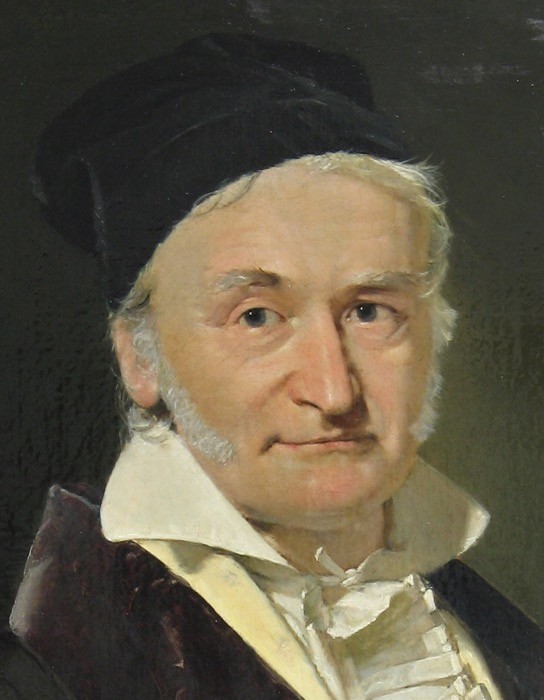
\includegraphics[height=0.62\textheight,keepaspectratio]{images/gauss_portrait.jpg}\\[2pt]
        {\scriptsize Carl Friedrich Gauß (1777--1855)\\
         G.\ Biermann nach C.\,A.\ Jensen\par}
      \end{center}
    \end{column}
    \begin{column}{0.65\textwidth}
      \begin{block}{Die Idee von Gauß}
        \begin{enumerate}
          \setlength{\itemsep}{3pt}
          \item Residuen \textbf{quadrieren}: nichts hebt sich auf.
          \item Quadrate \textbf{summieren}: $\sum \hat{u}_i^{\,2}$
          \item Gerade mit der \textbf{kleinsten} Summe wählen.
        \end{enumerate}
      \end{block}
      \begin{exampleblock}{Warum quadrieren?}
        Große Abweichungen zählen stärker: $3^{2} = 9$, aber $1^{2} = 1$.
      \end{exampleblock}
      \footnotesize Entwickelt von Gauß ab 1795.
    \end{column}
  \end{columns}
\end{frame}

% ---- Quadrierte Residuen als Flächen: A gegen D -------------------------
\begin{frame}{Quadrierte Residuen als Flächen}
  \begin{columns}[T]
    \begin{column}{0.31\textwidth}
      \begin{center}
      \begin{tikzpicture}
        \begin{axis}[regplot, scale only axis, height=3.544cm, width=2.59cm,
            xlabel={$x$ (Tsd.~Euro)}, ylabel={$y$ (Tsd.~Euro)},
            xmin=0, xmax=19, ymin=25, ymax=51, xtick={0,5,10,15}, ytick={25,30,...,50}]
          \quadratevon{\werbelist}{24}{2}{draw=resred, fill=resred, fill opacity=0.2, line width=0.8pt}
          \residuenvon{\werbelist}{24}{2}{resred, line width=1.4pt}
          \werbepunkte
          \addplot[hsbiaccent, thick, domain=0:14, samples=2] {24+2*x};
        \end{axis}
      \end{tikzpicture}\\[1pt]
      {\footnotesize Gerade A: $\sum \hat{u}_i^{\,2} = \mathbf{164{,}0}$}
      \end{center}
    \end{column}
    \begin{column}{0.31\textwidth}
      \begin{center}
      \begin{tikzpicture}
        \begin{axis}[regplot, scale only axis, height=3.544cm, width=2.59cm,
            xlabel={$x$ (Tsd.~Euro)}, ylabel={$y$ (Tsd.~Euro)},
            xmin=0, xmax=19, ymin=25, ymax=51, xtick={0,5,10,15}, ytick={25,30,...,50}]
          \quadratevon{\werbelist}{30}{1.2}{draw=resred, fill=resred, fill opacity=0.2, line width=0.8pt}
          \residuenvon{\werbelist}{30}{1.2}{resred, line width=1.4pt}
          \werbepunkte
          \addplot[hsbiblue, thick, domain=0:14, samples=2] {30+1.2*x};
        \end{axis}
      \end{tikzpicture}\\[1pt]
      {\footnotesize Gerade D: $\sum \hat{u}_i^{\,2} = \mathbf{64{,}8}$}
      \end{center}
    \end{column}
    \begin{column}{0.35\textwidth}
      \begin{block}{Konstruktion}
        Residuum $=$ Seite eines Quadrats mit Fläche $\hat{u}_i^{\,2}$.
      \end{block}
      \kernaussage{Gesucht: die Gerade mit der \textbf{kleinsten Gesamtfläche}.}
    \end{column}
  \end{columns}
\end{frame}

% ---- Das Minimierungsproblem ---------------------------------------------
\begin{frame}[label=minimierung]{Das Minimierungsproblem}
  \begin{block}{Residuenquadratsumme für beliebige $\beta_0$ und $\beta_1$}
    \vspace{-8pt}
    \begin{align*}
      S(\beta_0,\beta_1)
        &= \sum_{i=1}^{n}\bigl(\,y_i - \beta_0 - \beta_1 x_i\,\bigr)^{2}
           \uncover<2->{= \sum_{i=1}^{n}\Bigl(\,y_i - \underbrace{(\beta_0 + \beta_1 x_i)}_{=\,\hat{y}_i}\,\Bigr)^{2}}\\
        &\uncover<3->{= \sum_{i=1}^{n}\bigl(\,\underbrace{y_i - \hat{y}_i}_{=\,\hat{u}_i}\,\bigr)^{2}
           = \sum_{i=1}^{n}\hat{u}_i^{\,2}}
    \end{align*}
    \vspace{-8pt}

    z.\,B.\ $S(23;\,1) = 24$, \ $S(20;\,2) = 14$ (Online-Shop); \ $S(30;\,1{,}2) = 64{,}8$ (Filialen, D)
  \end{block}

  \begin{columns}[T]
    \begin{column}{0.5\textwidth}
      \begin{block}{Gesucht}
        \vspace{-6pt}
        \[
          (\hat{\beta}_0,\hat{\beta}_1) \;=\;
          \underset{\beta_0,\,\beta_1}{\arg\min}\; S(\beta_0,\beta_1)
        \]
        \vspace{-7pt}
      \end{block}
    \end{column}
    \begin{column}{0.48\textwidth}
      \textbf{In Worten:} die Werte $\beta_0$, $\beta_1$ mit der kleinsten
      Residuenquadratsumme.\\[4pt]
      {\footnotesize Im Minimum ist die Ableitung nach $\beta_0$ ($\beta_1$ fest) und nach
        $\beta_1$ ($\beta_0$ fest) null: die \emph{partiellen} Ableitungen.\par}
    \end{column}
  \end{columns}
\end{frame}

% ---- Der Lösungsweg in vier Schritten (Details im Anhang) ---------------
\begin{frame}[label=loesungsweg]{Vom Minimierungsproblem zum KQ-Schätzer in vier Schritten}
  \begin{center}
    \begin{tikzpicture}[>=Latex, font=\small,
        box/.style={draw=hsbibluedark, fill=hsbiblue!8, rounded corners=3pt,
                    minimum height=3.0cm, text width=2.15cm, align=center, inner sep=4pt},
        lab/.style={font=\footnotesize\bfseries, text=hsbibluedark, anchor=south, yshift=2pt},
        pfeil/.style={->, very thick, hsbibluedark}]
      \node[box] (b1) at (0,0) {$\dfrac{\partial S}{\partial \beta_0}$, \ $\dfrac{\partial S}{\partial \beta_1}$\\[4pt] {\footnotesize Kettenregel}};
      \node[box, right=0.5cm of b1, visible on=<2->] (b2) {(I) \ $\dfrac{\partial S}{\partial \beta_0} = 0$\\[3pt] (II) \ $\dfrac{\partial S}{\partial \beta_1} = 0$\\[3pt] {\footnotesize Normal-\\gleichungen}};
      \node[box, right=0.5cm of b2, visible on=<3->] (b3) {$\hat{\beta}_0 = \bar{y} - \hat{\beta}_1\,\bar{x}$\\[4pt] {\footnotesize (I) nach $\beta_0$ auflösen}};
      \node[box, right=0.5cm of b3, text width=4.05cm, visible on=<4->] (b4) {$\hat{\beta}_1 = \dfrac{\tsum (x_i - \bar{x})(y_i - \bar{y})}{\tsum (x_i - \bar{x})^{2}}$\\[4pt] {\footnotesize $\hat{\beta}_0$ in (II) einsetzen,\\ nach $\beta_1$ auflösen}};
      \node[lab] at (b1.north) {1.\ Ableiten};
      \node[lab, visible on=<2->] at (b2.north) {2.\ Null setzen};
      \node[lab, visible on=<3->] at (b3.north) {3.\ Auflösen};
      \node[lab, visible on=<4->] at (b4.north) {4.\ Einsetzen};
      \draw[pfeil, visible on=<2->] (b1) -- (b2);
      \draw[pfeil, visible on=<3->] (b2) -- (b3);
      \draw[pfeil, visible on=<4->] (b3) -- (b4);
    \end{tikzpicture}
  \end{center}

  \uncover<4->{\begin{block}{Schritt 4 genauer: Was heißt \glqq in (II) einsetzen\grqq?}
    \small
    (II) ausgeschrieben, durch $-2$ geteilt: \ $\sum x_i\,(y_i - \beta_0 - \beta_1 x_i) = 0$ \ -- zwei Unbekannte, $\beta_0$ und $\beta_1$.\\[2pt]
    $\beta_0 = \bar{y} - \beta_1\bar{x}$ aus Schritt 3 einsetzen: \
    $\sum x_i\,\bigl(y_i - (\bar{y} - \beta_1\bar{x}) - \beta_1 x_i\bigr) = 0$\\[2pt]
    Jetzt fehlt nur noch $\beta_1$ $\Rightarrow$ nach $\beta_1$ auflösen; das ergibt die Formel rechts oben.
  \end{block}}
  \hfill\hyperlink{herleitung}{\beamergotobutton{Jeder Rechenschritt: Herleitung im Anhang}}
\end{frame}

% ---- Die Lösung: KQ-Schätzer für die Steigung ------------------------------
\begin{frame}{Die Lösung des Minimierungsproblems: der KQ-Schätzer}
  \begin{block}{KQ-Schätzer für die Steigung}
    \[
      \hat{\beta}_1
      \;=\;
      \frac{\sum_{i=1}^{n} (x_i - \bar{x})(y_i - \bar{y})}
           {\sum_{i=1}^{n} (x_i - \bar{x})^{2}}
    \]
  \end{block}

  \medskip

  \begin{columns}[T]
    \begin{column}{0.49\textwidth}
      \begin{block}{Zähler}
        Summe der Abweichungsprodukte:\\ positiv bei steigender Punktwolke
      \end{block}
    \end{column}
    \begin{column}{0.49\textwidth}
      \begin{block}{Nenner}
        Summe der Abweichungsquadrate von $x$:\\ Streuung von $x$, $> 0$ (nicht alle $x_i$ gleich)
      \end{block}
    \end{column}
  \end{columns}

  \medskip

  \leitfrage{Kommen Ihnen Zähler und Nenner bekannt vor?}
\end{frame}

% ---- F2a: Verbindung zu Kovarianz und Varianz ----------------
\begin{frame}{Die Verbindung zu Kovarianz und Varianz}
  \begin{columns}[T]
    \begin{column}{0.49\textwidth}
      \begin{block}{Empirische Kovarianz}
        \[
          s_{xy} \;=\; {\color{hsbiaccent}\frac{1}{n-1}}
          \sum_{i=1}^{n} (x_i - \bar{x})(y_i - \bar{y})
        \]
      \end{block}
    \end{column}
    \begin{column}{0.49\textwidth}
      \begin{block}{Empirische Varianz von $x$}
        \[
          s_x^{2} \;=\; {\color{hsbiaccent}\frac{1}{n-1}}
          \sum_{i=1}^{n} (x_i - \bar{x})^{2}
        \]
      \end{block}
    \end{column}
  \end{columns}

  \begin{block}{Den Schätzer mit ${\color{hsbiaccent}1/(n-1)}$ erweitern}
    \[
      \hat{\beta}_1
      \;=\;
      \frac{{\color{hsbiaccent}\frac{1}{n-1}}\sum_{i=1}^{n}(x_i-\bar{x})(y_i-\bar{y})}
           {{\color{hsbiaccent}\frac{1}{n-1}}\sum_{i=1}^{n}(x_i-\bar{x})^{2}}
      \;=\;
      \frac{s_{xy}}{s_x^{2}}
    \]
  \end{block}
  \vspace{-4pt}
  \begin{center}
    \fbox{\rule[-6pt]{0pt}{20pt}\quad$\displaystyle \hat{\beta}_1 = \frac{s_{xy}}{s_x^{2}}$\quad}
  \end{center}
\end{frame}

% ---- F2b: Intuition und Beispiel -----------------------------
\begin{frame}{Steigung $=$ Kovarianz durch Varianz}
  \kernaussage{Steigung $=$ \textbf{Kovarianz} von $x$ und $y$ geteilt durch die
    \textbf{Varianz} von $x$.}

  \medskip

  \begin{columns}[T]
    \begin{column}{0.5\textwidth}
      \begin{block}{Intuition}
        \begin{itemize}
          \item $s_{xy}$: gemeinsame Variation
          \item $s_x^{2}$: Streuung von $x$ selbst
          \item Verhältnis: Änderung von $y$ je Einheit $x$
        \end{itemize}
      \end{block}
    \end{column}
    \begin{column}{0.48\textwidth}
      \begin{exampleblock}{Zwölf Filialen}
        \renewcommand{\arraystretch}{1.6}
        \begin{tabular}{@{}l@{}}
          $\hat{\beta}_1 = \dfrac{\SPxy}{\SQx} = \dfrac{186}{155} = 1{,}2$ \\
          $\hat{\beta}_1 = \dfrac{s_{xy}}{s_x^{2}} = \dfrac{186/11}{155/11} = \dfrac{16{,}91}{14{,}09} = 1{,}2$
        \end{tabular}
      \end{exampleblock}
    \end{column}
  \end{columns}
\end{frame}

% ---- Achsenabschnitt und Schwerpunkt -----------------------------------
\begin{frame}{Achsenabschnitt, KQ-Gerade und Antwort}
  \begin{columns}[T]
    \begin{column}{0.43\textwidth}
      \begin{tikzpicture}
        \begin{axis}[regplot, height=4.3cm, width=6.3cm, yticklabel shift=2pt]
          \werbepunkte
          \addplot[hsbiblue, thick, domain=0:14, samples=2] {30+1.2*x};
          \draw[hsbigray, dashed] (axis cs:7.5,24) -- (axis cs:7.5,39) -- (axis cs:0,39);
          \addplot[only marks, mark=square*, mark size=3pt, hsbiaccent] coordinates {(7.5,39)};
          \node[hsbiaccent, font=\footnotesize, anchor=north west, fill=white, inner sep=1pt, xshift=2pt, yshift=-2pt] at (axis cs:7.7,38.6) {$(\bar{x},\bar{y})$};
          \addplot[only marks, mark=*, mark size=2.6pt, hsbiaccent] coordinates {(0,30)};
          \node[hsbiaccent, font=\footnotesize, anchor=west, fill=white, inner sep=1pt, xshift=2pt] at (axis cs:0.3,27.6) {$\hat{\beta}_0 = 30$};
          \node[hsbigray, font=\footnotesize, anchor=south west, fill=white, inner sep=1pt, xshift=2pt, yshift=2pt] at (axis cs:7.7,24.2) {$\bar{x}$};
          \node[hsbigray, font=\footnotesize, anchor=west, fill=white, inner sep=1pt, xshift=2pt, yshift=1pt] at (axis cs:0.3,40.2) {$\bar{y}$};
        \end{axis}
      \end{tikzpicture}
    \end{column}
    \begin{column}{0.55\textwidth}
      \begin{block}{KQ-Schätzer: \ $\hat{\beta}_0 = \bar{y} - \hat{\beta}_1\,\bar{x}$}
        Gerade durch den \textbf{Schwerpunkt} $(\bar{x},\bar{y}) = (7{,}5;\,39)$
      \end{block}
      \begin{exampleblock}{Zwölf Filialen: beide Schätzer}
        Steigung: \ $\hat{\beta}_1 = \SPxy/\SQx = 186/155 = \mathbf{1{,}2}$\\[2pt]
        Achsenabschnitt: \ $\hat{\beta}_0 = 39 - 1{,}2 \cdot 7{,}5 = \mathbf{30}$\\[2pt]
        Regressionsgerade: \ $\hat{y} = 30 + 1{,}2\,x$
      \end{exampleblock}
    \end{column}
  \end{columns}

  \begin{exampleblock}{Antwort auf die Ausgangsfrage}
    $+1$ Tsd.~Euro Werbung bringt im Mittel $+1{,}2$ Tsd.~Euro Umsatz.\\
    Bei $7$ Tsd.~Euro Werbung: \ $\hat{y} = 30 + 1{,}2 \cdot 7 = \mathbf{38{,}4}$ Tsd.~Euro.
  \end{exampleblock}
  {\footnotesize Jede Gerade durch $(\bar{x},\bar{y})$ hat die Residuensumme $0$ -- auch beide Geraden aus Übung (3).\par}
\end{frame}

% ---- Beide Schätzer im Überblick ----------------------------------------
\begin{frame}{Beide Schätzer im Überblick}
  \begin{block}{Die KQ-Gerade}
    \vspace{-4pt}
    \[
      \hat{\beta}_1 = \frac{s_{xy}}{s_x^{2}}
      \qquad\qquad
      \hat{\beta}_0 = \bar{y} - \hat{\beta}_1\,\bar{x}
      \qquad\qquad
      \hat{y}_i = \hat{\beta}_0 + \hat{\beta}_1\, x_i
    \]
    \vspace{-10pt}
  \end{block}

  \medskip

  \begin{columns}[T]
    \begin{column}{0.52\textwidth}
      \begin{exampleblock}{Antwort auf die Ausgangsfrage}
        $\hat{y} = 30 + 1{,}2\,x$ \ (Gerade D)\\[2pt]
        $+1$ Tsd.~Euro Werbung: $+1{,}2$ Tsd.~Euro Umsatz\\
        $x = 7$: \ $\hat{y} = 38{,}4$ Tsd.~Euro
      \end{exampleblock}
    \end{column}
    \begin{column}{0.46\textwidth}
      \begin{block}{Eigenschaften}
        \begin{itemize}
          \item durch $(\bar{x}, \bar{y})$
          \item $\sum \hat{u}_i = 0$ \ und \ $\sum x_i\,\hat{u}_i = 0$\\
                {\footnotesize (aus den Ableitungen nach $\beta_0$ und $\beta_1$)}
        \end{itemize}
      \end{block}
    \end{column}
  \end{columns}
  \hfill\hyperlink{herleitung}{\beamergotobutton{Herleitung}}
\end{frame}

% ---- G: Schritt-für-Schritt ----------------------------------
\begin{frame}{Schritt für Schritt zur Regressionsgeraden}
  \begin{columns}[T]
    \begin{column}{0.4\textwidth}
      \begin{block}{Rechenschema}
        \small
        \begin{enumerate}
          \setlength{\itemsep}{1pt}
          \item Mittelwerte $\bar{x}$, $\bar{y}$
          \item Kovarianz $s_{xy} = \sum (x_i-\bar{x})(y_i-\bar{y}) / (n-1)$
          \item Varianz $s_x^{2} = \sum (x_i-\bar{x})^{2} / (n-1)$
          \item Steigung $\hat{\beta}_1 = s_{xy} / s_x^{2}$
          \item Achsenabschnitt $\hat{\beta}_0 = \bar{y} - \hat{\beta}_1 \bar{x}$
          \item Gerade $\hat{y} = \hat{\beta}_0 + \hat{\beta}_1 x$
        \end{enumerate}
      \end{block}
      \footnotesize Bei vielen Daten: Rechenabkürzung über Summen (Anhang).
    \end{column}
    \begin{column}{0.58\textwidth}
      \begin{block}{Arbeitstabelle für die Schritte 2 und 3}
        \begin{center}
          \scriptsize
          \renewcommand{\arraystretch}{1.2}
          \setlength{\tabcolsep}{3pt}
          \begin{tabular}{ccccccc}
            \toprule
            $i$ & $x_i$ & $y_i$ & $x_i-\bar{x}$ & $y_i-\bar{y}$ & $(x_i-\bar{x})(y_i-\bar{y})$ & $(x_i-\bar{x})^{2}$ \\
            \midrule
            1 & & & & & & \\
            2 & & & & & & \\
            $\vdots$ & & & & & & \\
            $n$ & & & & & & \\
            \midrule
            $\sum$ & & & $0$ & $0$ & $\to s_{xy}$ & $\to s_x^{2}$ \\
            \bottomrule
          \end{tabular}
        \end{center}
        \small Kontrolle: Spalten $x_i-\bar{x}$, $y_i-\bar{y}$ ergeben $0$.
      \end{block}
    \end{column}
  \end{columns}
\end{frame}

% ---- Übung Online-Shop (5): KQ-Gerade für einen zweiten Shop --------------
\begin{frame}{Übung Online-Shop (5): Die KQ-Gerade für einen zweiten Shop}
  \begin{columns}[T]
    \begin{column}{0.5\textwidth}
      \begin{block}{Situation}
        Der Händler eröffnet einen zweiten Shop: fünf Monate, Werte in Tsd.~Euro.
      \end{block}
      \begin{exampleblock}{Aufgaben}
        \small
        \begin{enumerate}[a)]
          \setlength{\itemsep}{2pt}
          \item $\bar{x}$, $\bar{y}$, $\SPxy$ und $\SQx$ mit einer Arbeitstabelle berechnen.
          \item $\hat{\beta}_1 = \SPxy/\SQx$ und $\hat{\beta}_0 = \bar{y} - \hat{\beta}_1\bar{x}$ bestimmen;
                Regressionsgerade angeben.
          \item Die Steigung in Worten deuten.
          \item $\hat{y}_i$ und $\hat{u}_i$ berechnen; $\sum \hat{u}_i = 0$ prüfen.
          \item Gerade ins Streuungsdiagramm einzeichnen.
        \end{enumerate}
      \end{exampleblock}
    \end{column}
    \begin{column}{0.48\textwidth}
      \begin{center}
        \small
        \renewcommand{\arraystretch}{1.1}
        \begin{tabular}{l*{5}{r}}
          \toprule
          Monat $i$            & 1  & 2  & 3  & 4  & 5  \\
          \midrule
          Werbeaufwand $x_i$   & 2  & 4  & 5  & 6  & 8  \\
          Umsatz $y_i$         & 12 & 20 & 19 & 23 & 31 \\
          \bottomrule
        \end{tabular}
      \end{center}
      \begin{tikzpicture}
        \begin{axis}[uebBplot, height=3.85cm, width=6.8cm]
          \uebBpunkte
        \end{axis}
      \end{tikzpicture}
    \end{column}
  \end{columns}
\end{frame}

% ---- Lösung Online-Shop (5), Teil 1 -----------------------------------------
\begin{frame}{Lösung Online-Shop (5), Teil 1: Arbeitstabelle und KQ-Schätzer}
  \begin{block}{a) Regel: Mittelwerte, dann Abweichungen, Produkte und Quadrate summieren}
    \vspace{-4pt}
    \begin{center}
      \footnotesize
      \renewcommand{\arraystretch}{0.95}
      \begin{tabular}{crrrrrr}
        \toprule
        $i$ & $x_i$ & $y_i$ & $x_i - \bar{x}$ & $y_i - \bar{y}$ & $(x_i - \bar{x})(y_i - \bar{y})$ & $(x_i - \bar{x})^{2}$ \\
        \midrule
        1 & 2 & 12 & $-3$ & $-9$ & $27$ & $9$ \\
        2 & 4 & 20 & $-1$ & $-1$ & $1$  & $1$ \\
        3 & 5 & 19 & $0$  & $-2$ & $0$  & $0$ \\
        4 & 6 & 23 & $1$  & $2$  & $2$  & $1$ \\
        5 & 8 & 31 & $3$  & $10$ & $30$ & $9$ \\
        \midrule
        $\sum$ & 25 & 105 & $0$ & $0$ & $\SPxy = \mathbf{60}$ & $\SQx = \mathbf{20}$ \\
        \bottomrule
      \end{tabular}
    \end{center}
    \small $\bar{x} = 25/5 = \mathbf{5}$, \quad $\bar{y} = 105/5 = \mathbf{21}$; \quad
    Kontrolle: Die Abweichungen summieren sich zu $0$.
  \end{block}
  \vspace{-4pt}

  \begin{columns}[T]
    \begin{column}{0.58\textwidth}
      \begin{block}{b) Regel: $\hat{\beta}_1 = \SPxy/\SQx$, \ $\hat{\beta}_0 = \bar{y} - \hat{\beta}_1\,\bar{x}$}
        $\hat{\beta}_1 = 60/20 = \mathbf{3}$, \ \ $\hat{\beta}_0 = 21 - 3 \cdot 5 = \mathbf{6}$
        \ $\Rightarrow$ \ $\hat{y} = 6 + 3\,x$
      \end{block}
    \end{column}
    \begin{column}{0.4\textwidth}
      \begin{exampleblock}{c) Deutung der Steigung}
        $+1$ Tsd.~Euro Werbung: $+3$ Tsd.~Euro Umsatz (im Mittel).
      \end{exampleblock}
    \end{column}
  \end{columns}
\end{frame}

% ---- Lösung Online-Shop (5), Teil 2 -----------------------------------------
\begin{frame}{Lösung Online-Shop (5), Teil 2: Residuen und Grafik}
  \begin{columns}[T]
    \begin{column}{0.5\textwidth}
      \begin{tikzpicture}
        \begin{axis}[uebBplot, height=5.0cm, width=7.2cm]
          \residuenvon{\uebBliste}{6}{3}{resred, line width=1.4pt}
          \uebBpunkte
          \addplot[hsbiblue, thick, domain=0:9, samples=2] {6+3*x};
          \addplot[only marks, mark=square*, mark size=3pt, hsbiaccent] coordinates {(5,21)};
          \node[hsbiaccent, font=\footnotesize, anchor=south east, fill=white, inner sep=1pt] at (axis cs:4.8,21.6) {$(\bar{x},\bar{y})$};
          \node[hsbiblue, font=\footnotesize, anchor=north west, fill=white, inner sep=1pt] at (axis cs:6.5,20.5) {$\hat{y} = 6 + 3x$};
        \end{axis}
      \end{tikzpicture}
      \begin{center}\footnotesize
        e) Die Gerade geht durch den Schwerpunkt $(5;\,21)$.
      \end{center}
    \end{column}
    \begin{column}{0.48\textwidth}
      \begin{block}{d) Regel: $\hat{y}_i = 6 + 3\,x_i$, \ $\hat{u}_i = y_i - \hat{y}_i$}
        \begin{center}
          \footnotesize
          \renewcommand{\arraystretch}{0.95}
          \begin{tabular}{ccccr}
            \toprule
            $i$ & $x_i$ & $y_i$ & $\hat{y}_i$ & $\hat{u}_i$ \\
            \midrule
            1 & 2 & 12 & $6 + 3 \cdot 2 = 12$ & $0$  \\
            2 & 4 & 20 & $6 + 3 \cdot 4 = 18$ & $2$  \\
            3 & 5 & 19 & $6 + 3 \cdot 5 = 21$ & $-2$ \\
            4 & 6 & 23 & $6 + 3 \cdot 6 = 24$ & $-1$ \\
            5 & 8 & 31 & $6 + 3 \cdot 8 = 30$ & $1$  \\
            \midrule
            $\sum$ & & & & $\mathbf{0}$ \checkmark \\
            \bottomrule
          \end{tabular}
        \end{center}
      \end{block}
      \begin{exampleblock}{Zum Vergleich: der erste Shop}
        \small $\hat{\beta}_1 = 20/10 = 2$, \ $\hat{\beta}_0 = 26 - 2 \cdot 3 = 20$:
        \ $\hat{y} = 20 + 2\,x$ ist \textbf{Gerade 2} aus Übung (3).
      \end{exampleblock}
    \end{column}
  \end{columns}
\end{frame}

% ===== SUBSECTION: INTERPRETATION =====
\subsection{Interpretation}

% ---- I1: Steigung ---------------------------------------------
\begin{frame}{Wie interpretieren wir die Steigung?}
  \begin{columns}[T]
    \begin{column}{0.53\textwidth}
      \begin{tikzpicture}
        \begin{axis}[uebplot, height=5.9cm, width=7.9cm]
          \uebpunkte
          \addplot[hsbiblue, thick, domain=0:6, samples=2] {20+2*x};
          \draw[hsbigray, dashed] (axis cs:2,16) -- (axis cs:2,24) -- (axis cs:0,24);
          \draw[hsbigray, dashed] (axis cs:3,16) -- (axis cs:3,26) -- (axis cs:0,26);
          \draw[hsbigreen, very thick] (axis cs:2,24) -- (axis cs:3,24) -- (axis cs:3,26);
          \node[hsbigreen, font=\footnotesize, below] at (axis cs:2.5,24) {$+1$};
          \node[hsbigreen, font=\footnotesize, right] at (axis cs:3,25.4) {$+2 = \hat{\beta}_1$};
          \addplot[only marks, mark=o, mark size=2.6pt, line width=1pt, hsbibluedark] coordinates {(2,24) (3,26)};
          \node[hsbiblue, font=\footnotesize, anchor=north west, fill=white, inner sep=1pt] at (axis cs:0.15,33.6) {$\hat{y} = 20 + 2x$ (KQ-Gerade Online-Shop)};
        \end{axis}
      \end{tikzpicture}
    \end{column}
    \begin{column}{0.45\textwidth}
      \begin{block}{Steigung $\hat{\beta}_1 = 2$}
        $x$ steigt um $1$ \ $\Rightarrow$ \ $\hat{y}$ steigt um $\hat{\beta}_1$\\[3pt]
        Hier: $x = 2 \to 3$, \ $\hat{y} = 24 \to 26$
      \end{block}
      \begin{exampleblock}{In Worten}
        $2$ Tsd.~Euro mehr Umsatz je Tsd.~Euro Werbung (laut Gerade).
      \end{exampleblock}
      \begin{alertblock}{Keine kausale Aussage}
        Statistischer Zusammenhang -- kein Beweis für eine Wirkung.
      \end{alertblock}
    \end{column}
  \end{columns}
\end{frame}

% ---- I2: Achsenabschnitt --------------------------------------
\begin{frame}{Wie interpretieren wir den Achsenabschnitt?}
  \begin{columns}[T]
    \begin{column}{0.53\textwidth}
      \begin{tikzpicture}
        \begin{axis}[uebplot, height=5.9cm, width=7.9cm, yticklabel shift=2pt]
          \uebpunkte
          \addplot[hsbiblue, thick, domain=0:6, samples=2] {20+2*x};
          \addplot[only marks, mark=*, mark size=3pt, hsbiaccent] coordinates {(0,20)};
          \draw[hsbigray, dashed] (axis cs:1,16) -- (axis cs:1,34);
          \draw[hsbigray, dashed] (axis cs:5,16) -- (axis cs:5,34);
          \node[hsbiaccent, font=\footnotesize, anchor=west, fill=white, inner sep=1pt] at (axis cs:0.2,18.8) {$\hat{\beta}_0 = 20$};
          \draw[hsbigray, <->, >=Latex] (axis cs:1,31.6) -- (axis cs:5,31.6);
          \node[hsbigray, font=\footnotesize, anchor=south, fill=white, inner sep=1pt] at (axis cs:3,31.7) {beobachteter Bereich};
        \end{axis}
      \end{tikzpicture}
    \end{column}
    \begin{column}{0.45\textwidth}
      \begin{block}{Achsenabschnitt $\hat{\beta}_0 = 20$}
        $\hat{y}$ bei $x = 0$: Umsatz ohne Werbung
      \end{block}
      \begin{alertblock}{Vorsicht}
        \begin{itemize}
          \item $x = 0$ nicht beobachtet (Daten: $1$~bis~$5$): \emph{Extrapolation}
          \item weit außerhalb der Daten: oft ohne inhaltliche Bedeutung
        \end{itemize}
      \end{alertblock}
    \end{column}
  \end{columns}
\end{frame}

% ---- Interpretation im Überblick und Prognosen ---------------------------
\begin{frame}{Interpretation im Überblick -- und Prognosen}
  \begin{columns}[T]
    \begin{column}{0.5\textwidth}
      \begin{tikzpicture}
        \begin{axis}[uebplot, height=5.8cm, width=7.4cm, yticklabel shift=2pt]
          \uebpunkte
          \addplot[hsbiblue, thick, domain=0:6, samples=2] {20+2*x};
          \addplot[only marks, mark=*, mark size=3pt, hsbiaccent] coordinates {(0,20)};
          \node[hsbiaccent, font=\footnotesize, anchor=west, fill=white, inner sep=1pt, xshift=2pt] at (axis cs:0.2,18.8) {$\hat{\beta}_0 = 20$};
          \draw[hsbigreen, very thick] (axis cs:2,24) -- (axis cs:3,24) -- (axis cs:3,26);
          \node[hsbigreen, font=\footnotesize, right] at (axis cs:3,25.2) {$\hat{\beta}_1 = 2$};
          % Prognose bei x = 4,5
          \draw[resred, dashed, visible on=<2->] (axis cs:4.5,16) -- (axis cs:4.5,29) -- (axis cs:0,29);
          \addplot[only marks, mark=square*, mark size=3pt, resred, visible on=<2->] coordinates {(4.5,29)};
          \node[resred, font=\footnotesize, anchor=south, fill=white, inner sep=1pt, visible on=<2->] at (axis cs:1.2,29.2) {$\hat{y} = 29$};
          \node[hsbiblue, font=\footnotesize, anchor=south east] at (axis cs:5.9,31.5) {$\hat{y} = 20 + 2x$};
        \end{axis}
      \end{tikzpicture}
    \end{column}
    \begin{column}{0.48\textwidth}
      \begin{block}{$\hat{y} = {\color{hsbiaccent}20} + {\color{hsbigreen}2}\,x$}
        \begin{description}[$\hat{\beta}_1$]
          \item[{\color{hsbiaccent}$\hat{\beta}_0$}] Höhe der Geraden bei $x = 0$
          \item[{\color{hsbigreen}$\hat{\beta}_1$}] $\Delta \hat{y} = \hat{\beta}_1 \cdot \Delta x$ \ ($\Delta$: Änderung)
        \end{description}
      \end{block}
      \uncover<2->{\begin{exampleblock}{Prognose: $x$ einsetzen}
        $x = 4{,}5$: \ $\hat{y} = 29$ \ -- \textbf{Interpolation}\\[3pt]
        $x = 20$: \ $\hat{y} = 60$ \ -- \textbf{Extrapolation}!
      \end{exampleblock}}
    \end{column}
  \end{columns}
\end{frame}

% ---- Leuchte: Berechnung mit bekannten Kennzahlen -------------------------
\begin{frame}{Zweites Beispiel: Preis und Absatz der Leuchte}
  \begin{columns}[T]
    \begin{column}{0.52\textwidth}
      \begin{tikzpicture}
        \begin{axis}[leuchteplot, height=5.9cm, width=7.8cm]
          \residuenvon{\leuchteliste}{54.6667}{-0.44667}{resred, line width=1.2pt}
          \leuchtepunkte
          \addplot[hsbiblue, thick, domain=75:125, samples=2] {54.6667-0.44667*x};
          \node[hsbiblue, font=\footnotesize, anchor=north east, fill=white, inner sep=1pt] at (axis cs:124,21) {$\hat{y} = 54{,}67 - 0{,}4467\,x$};
        \end{axis}
      \end{tikzpicture}
    \end{column}
    \begin{column}{0.46\textwidth}
      \begin{block}{Schritte 1--3: schon bekannt}
        $\bar{x} = 100$, \ $\bar{y} = 10$, \ $s_{xy} = -83{,}75$, \ $s_x^{2} = 187{,}5$
      \end{block}
      \begin{block}{Schritte 4--6}
        $\hat{\beta}_1 = -83{,}75 / 187{,}5 = \mathbf{-0{,}4467}$\\[2pt]
        $\hat{\beta}_0 = 10 + 0{,}4467 \cdot 100 = \mathbf{54{,}67}$
      \end{block}
      \begin{exampleblock}{Antwort auf die Frage vom Beginn}
        $+10$ Euro: \ $-4{,}5$ Stück \ ($10 \cdot 0{,}4467$)\\
        Prognose bei $98$ Euro: $\hat{y} = 10{,}89$ Stück
      \end{exampleblock}
    \end{column}
  \end{columns}
\end{frame}

% ---- Leuchte: Interpretation, Extrapolation sichtbar ------------------------
\begin{frame}{Preis und Absatz: Interpretation der Koeffizienten}
  \begin{columns}[T]
    \begin{column}{0.52\textwidth}
      \begin{tikzpicture}
        \begin{axis}[regbasis, height=5.9cm, width=7.8cm,
            xlabel={Preis $x$ (Euro)}, ylabel={Absatzmenge $y$ (Stück)},
            xmin=0, xmax=130, ymin=0, ymax=62, xtick={0,20,...,120}, ytick={0,10,...,60}]
          \fill[hsbiblue!10] (axis cs:80,0) rectangle (axis cs:120,62);
          \node[hsbibluedark, font=\scriptsize, align=center] at (axis cs:100,55) {beobachteter\\ Bereich};
          \addplot[hsbiblue, thick, dashed, domain=0:80, samples=2] {54.6667-0.44667*x};
          \addplot[hsbiblue, thick, domain=80:122, samples=2] {54.6667-0.44667*x};
          \leuchtepunkte
          \addplot[only marks, mark=*, mark size=3pt, hsbiaccent] coordinates {(0,54.6667)};
          \node[hsbiaccent, font=\footnotesize, anchor=south west, fill=white, inner sep=1pt] at (axis cs:2,56.5) {$\hat{\beta}_0 = 54{,}67$};
          \node[hsbigray, font=\footnotesize, anchor=north east, fill=white, inner sep=1pt] at (axis cs:60,24) {Extrapolation};
        \end{axis}
      \end{tikzpicture}
    \end{column}
    \begin{column}{0.46\textwidth}
      \begin{block}{Steigung $\hat{\beta}_1 = -0{,}4467$}
        $+1$ Euro Preis: $0{,}45$ Stück weniger Absatz -- eine fallende
        Preis-Absatz-Funktion
      \end{block}
      \begin{alertblock}{Achsenabschnitt $\hat{\beta}_0 = 54{,}67$}
        Absatz bei $0$ Euro -- weit außerhalb der Daten ($80$ bis $120$ Euro):
        \textbf{nicht interpretierbar}
      \end{alertblock}
    \end{column}
  \end{columns}
\end{frame}

% ---- R ---------------------------------------------------------
\begin{frame}[fragile]{Lineare Regression mit R}
  \begin{block}{Koeffizienten manuell (Schritte 2 bis 5)}
\begin{lstlisting}
(beta1 <- cov(preis, menge) / var(preis))
(beta0 <- mean(menge) - beta1 * mean(preis))
\end{lstlisting}
  \end{block}

  \begin{block}{Dasselbe mit der Funktion \texttt{lm()} (\emph{linear model})}
\begin{lstlisting}
reg <- lm(menge ~ preis)
coef(reg)                      # Achsenabschnitt und Steigung
\end{lstlisting}
  \end{block}

  \begin{block}{Streuungsdiagramm mit Regressionsgeraden}
\begin{lstlisting}
plot(preis, menge, xlim = c(0, 125), ylim = c(0, 60))
abline(reg)
\end{lstlisting}
  \end{block}
\end{frame}

% ---- Ü-I: Übungsaufgabe Interpretation und Prognose -------------
\begin{frame}{Übung Möbelhaus: Koeffizienten deuten und Prognosen ableiten}
  \begin{block}{Möbelhaus, sechs Wochen (Tsd.~Euro) -- KQ-Gerade $\hat{y} = 40 + 2{,}5\,x$}
    \begin{center}
      \renewcommand{\arraystretch}{1.05}
      \begin{tabular}{l*{6}{r}}
        \toprule
        Werbeausgaben $x_i$ & 2  & 4  & 6  & 8  & 10 & 12 \\
        Wochenumsatz $y_i$  & 44 & 49 & 58 & 62 & 61 & 71 \\
        \bottomrule
      \end{tabular}
    \end{center}
  \end{block}

  \medskip

  \begin{exampleblock}{Aufgaben}
    \begin{enumerate}[a)]
      \setlength{\itemsep}{2pt}
      \item $\hat{\beta}_0$ und $\hat{\beta}_1$ mit Einheiten deuten. Ist $\hat{\beta}_0$ sinnvoll?
      \item Prognose für $x = 5$ und $x = 30$ -- wie belastbar?
      \item Änderung von $\hat{y}$ bei $x = 4 \to 6$ und bei $x = 10 \to 12$?
      \item $x$ in Euro statt Tsd.~Euro: neue $\hat{\beta}_0$, $\hat{\beta}_1$? Und zusätzlich $y$ in Euro?\\
            {\footnotesize Tipp: $x = x_{\text{Euro}} / 1000$ in die Gerade einsetzen.}
    \end{enumerate}
  \end{exampleblock}
\end{frame}

% ---- Ü-I Lösung 1 ------------------------------------------------
\begin{frame}{Lösung Möbelhaus (1/3): Koeffizienten deuten und Änderungen berechnen}
  \small

  \begin{columns}[T]
    \begin{column}{0.5\textwidth}
      \begin{block}{a) Regel: $\hat{\beta}_1$ = Änderung von $\hat{y}$ je Einheit $x$}
        $\hat{\beta}_1 = 2{,}5$: Je Tsd.~Euro Werbung laut Gerade \textbf{$2{,}5$ Tsd.~Euro} mehr
        Wochenumsatz -- kein Kausalbeweis.
      \end{block}
      \begin{block}{a) Regel: $\hat{\beta}_0$ = Wert von $\hat{y}$ bei $x = 0$}
        $\hat{\beta}_0 = 40$: Umsatz ohne Werbung \textbf{$40$ Tsd.~Euro}. $x = 0$ liegt knapp
        außerhalb der Daten ($2$ bis $12$): Extrapolation, grobe Orientierung.
      \end{block}
    \end{column}
    \begin{column}{0.48\textwidth}
      \begin{exampleblock}{c) Regel: $\Delta \hat{y} = \hat{\beta}_1 \cdot \Delta x$}
        $\Delta x = 2$: \ $\Delta \hat{y} = 2{,}5 \cdot 2 = \mathbf{5}$ Tsd.~Euro -- in beiden Fällen:\\[2pt]
        $4 \to 6$: \ $\hat{y}$ von $40 + 2{,}5 \cdot 4 = 50$ auf $55$\\
        $10 \to 12$: \ $\hat{y}$ von $65$ auf $70$\\[2pt]
        Gleicher Zuwachs: Eine Gerade hat überall dieselbe Steigung.
      \end{exampleblock}
    \end{column}
  \end{columns}
\end{frame}

% ---- Ü-I Lösung 2 ------------------------------------------------
\begin{frame}{Lösung Möbelhaus (2/3): Prognosen und ihre Grenzen}
  \begin{columns}[T]
    \begin{column}{0.5\textwidth}
      \begin{tikzpicture}
        \begin{axis}[regbasis, height=5.6cm, width=7.4cm,
            xlabel={Werbeausgaben $x$ (Tsd.~Euro)}, ylabel={Wochenumsatz $y$ (Tsd.~Euro)},
            xmin=0, xmax=14, ymin=35, ymax=86, xtick={0,2,...,14}, ytick={40,50,...,80}]
          \addplot[only marks, mark=*, mark size=2.4pt, hsbiblue]
            coordinates {(2,44) (4,49) (6,58) (8,62) (10,61) (12,71)};
          \addplot[hsbiblue, thick, domain=0:14, samples=2] {40+2.5*x};
          \draw[hsbigray, dashed] (axis cs:5,35) -- (axis cs:5,52.5) -- (axis cs:0,52.5);
          \addplot[only marks, mark=square*, mark size=3pt, hsbiaccent] coordinates {(5,52.5)};
          \node[hsbiaccent, font=\footnotesize, anchor=south east, fill=white, inner sep=1pt, xshift=-2pt, yshift=2pt] at (axis cs:4.8,53) {$52{,}5$};
          \draw[hsbigray, <->, >=Latex] (axis cs:2,83) -- (axis cs:12,83);
          \node[hsbigray, font=\footnotesize, anchor=north, fill=white, inner sep=1pt] at (axis cs:7,82.5) {beobachteter Bereich};
          \node[resred, font=\footnotesize, anchor=east, fill=white, inner sep=1pt] at (axis cs:13.9,38) {$x = 30$? $\rightarrow$};
        \end{axis}
      \end{tikzpicture}
    \end{column}
    \begin{column}{0.48\textwidth}
      \small
      \begin{block}{b) Regel: $x$ in die Gerade einsetzen}
        $x = 5$: \ $\hat{y} = 40 + 2{,}5 \cdot 5 = \mathbf{52{,}5}$ Tsd.~Euro\\[2pt]
        $x = 30$: \ $\hat{y} = 40 + 2{,}5 \cdot 30 = \mathbf{115}$ Tsd.~Euro
      \end{block}
      \begin{exampleblock}{$x = 5$: Interpolation}
        Im beobachteten Bereich ($2$ bis $12$): plausibel -- als Erwartung.
      \end{exampleblock}
      \begin{alertblock}{$x = 30$: Extrapolation}
        Weit außerhalb der Daten, Linearität dort unbekannt:
        \textbf{nicht belastbar}.
      \end{alertblock}
    \end{column}
  \end{columns}
\end{frame}

% ---- Ü-I Lösung 3 ------------------------------------------------
\begin{frame}[fragile]{Lösung Möbelhaus (3/3): Andere Einheiten -- und die Kontrolle mit R}
  \small\lstset{basicstyle=\ttfamily\footnotesize,aboveskip=2pt,belowskip=2pt}
  \begin{block}{d) Regel: Einheit von $x$ ändert $\hat{\beta}_1$, Einheit von $y$ beide Koeffizienten}
    \vspace{-2pt}
    $x$ in Euro ($x = x_{\text{Euro}}/1000$): \ $\hat{y} = 40 + 2{,}5 \cdot x_{\text{Euro}}/1000 = 40 + 0{,}0025\,x_{\text{Euro}}$\\
    $\Rightarrow$ $\hat{\beta}_1 = \mathbf{0{,}0025}$ (Tsd.~Euro je Euro), \ $\hat{\beta}_0 = \mathbf{40}$ unverändert\\[2pt]
    Zusätzlich $y$ in Euro (mal $1000$): \ $\hat{y}_{\text{Euro}} = \mathbf{40\,000} + \mathbf{2{,}5}\,x_{\text{Euro}}$\\
    $\Rightarrow$ je Euro Werbung $2{,}50$~Euro mehr Umsatz: \textbf{dieselbe Aussage}
  \end{block}

  \begin{exampleblock}{Kontrolle mit R}
\begin{lstlisting}
werbung <- c(2, 4, 6, 8, 10, 12); umsatz <- c(44, 49, 58, 62, 61, 71)
reg <- lm(umsatz ~ werbung)
coef(reg)                                            # 40.0   2.5
predict(reg, newdata = data.frame(werbung = c(5, 30)))   # 52.5 115.0
coef(lm(umsatz ~ I(1000 * werbung)))                 # 40.0000   0.0025
\end{lstlisting}
  \end{exampleblock}

\end{frame}

% ---- Rückblick -------------------------------------------------
\begin{frame}{Rückblick: Können Sie diese Fragen beantworten?}
  \begin{enumerate}
    \setlength{\itemsep}{5pt}
    \item Was messen Kovarianz und Korrelation -- und was nicht?
    \item Was leistet die Regression, was die Korrelation nicht leistet?
    \item Warum taugt die Summe der Residuen nicht als Kriterium?
    \item Welche Idee steckt hinter der Methode der kleinsten Quadrate?
    \item Wie berechnet man $\hat{\beta}_1$ und $\hat{\beta}_0$ von Hand?
    \item Wie interpretiert man die Parameter -- und was nicht?
  \end{enumerate}

  \medskip

  \kernaussage{KQ-Gerade: kleinste Residuenquadratsumme, berechnet aus $\bar{x}$,
    $\bar{y}$, $s_{xy}$ und $s_x^{2}$.}
\end{frame}

% ===== SUBSECTION: BESTIMMTHEITSMASS =====
\subsection{Bestimmtheitsmaß}

% ---- B1: Motivation ---------------------------------------------------
\begin{frame}{Wie viel erklärt die Gerade?}
  \begin{columns}[T]
    \begin{column}{0.49\textwidth}
      \begin{center}
      \begin{tikzpicture}
        \begin{axis}[regplot, height=4.7cm, width=6.9cm, title={\footnotesize Ohne $x$: Prognose $\bar{y} = 39$, \ $\sum (y_i - \bar{y})^{2} = \mathbf{288}$}, height=4.05cm]
          \residuenvon{\werbelist}{39}{0}{hsbigreen, line width=1.4pt}
          \werbepunkte
          \addplot[hsbigray, thick, dashed, domain=0:14, samples=2] {39};
          \node[hsbigray, font=\footnotesize, anchor=south west] at (axis cs:0.2,39.2) {$\bar{y}$};
        \end{axis}
      \end{tikzpicture}
      \end{center}
    \end{column}
    \begin{column}{0.49\textwidth}
      \begin{center}
      \begin{tikzpicture}
        \begin{axis}[regplot, height=4.7cm, width=6.9cm, title={\footnotesize Mit $x$: Prognose $\hat{y}_i$, \ $\sum \hat{u}_i^{\,2} = \mathbf{64{,}8}$}, height=4.05cm,
            visible on=<2->]
          \residuenvon{\werbelist}{30}{1.2}{resred, line width=1.4pt, visible on=<2->}
          \addplot[only marks, mark=*, mark size=2.2pt, color=hsbiblue, visible on=<2->]
            coordinates {(1,33) (3,30) (4,37) (5,33) (6,38) (8,41) (8,39) (9,43) (10,45) (11,40) (12,42) (13,47)};
          \addplot[hsbiblue, thick, domain=0:14, samples=2, visible on=<2->] {30+1.2*x};
        \end{axis}
      \end{tikzpicture}
      \end{center}
    \end{column}
  \end{columns}

  \small
  \only<1>{\leitfrage{Ohne $x$ ist $\bar{y}$ die beste Prognose. Wie viel besser wird es
    \emph{mit} der Geraden?}}%
  \only<2->{\kernaussage{Von $288$ auf $64{,}8$: Die Gerade erklärt
    $(288 - 64{,}8)/288 = \mathbf{77{,}5\,\%}$ der Streuung.}}
\end{frame}

% ---- B2: Eine Abweichung zerlegen --------------------------------------
\begin{frame}{Eine Abweichung in zwei Teile zerlegen}
  \begin{columns}[T]
    \begin{column}{0.55\textwidth}
      \begin{tikzpicture}
        \begin{axis}[regplot, height=6.0cm, width=8.0cm, xmax=16, xtick={0,2,...,16}, clip mode=individual]
          \werbepunkte
          \addplot[hsbiblue, thick, domain=0:16, samples=2] {30+1.2*x};
          \addplot[hsbigray, thick, dashed, domain=0:16, samples=2] {39};
          \node[hsbigray, font=\footnotesize, anchor=south west] at (axis cs:0.2,39.2) {$\bar{y} = 39$};
          % Gesamtabweichung: direkt neben dem Punkt, von der y-quer-Linie bis zur Höhe des Punktes
          \draw[hsbigreen, dashed, visible on=<1->] (axis cs:13,47) -- (axis cs:13.55,47);
          \draw[hsbigreen, line width=2pt, visible on=<1->] (axis cs:13.55,39) -- (axis cs:13.55,47);
          \node[hsbigreen, font=\footnotesize\bfseries, anchor=west, fill=white, inner sep=1pt, visible on=<1->] at (axis cs:13.75,43) {$8$};
          % erklärter Teil
          \draw[hsbiaccent, line width=2pt, visible on=<2->] (axis cs:13,39) -- (axis cs:13,45.6);
          \node[hsbiaccent, font=\footnotesize\bfseries, anchor=east, fill=white, inner sep=1pt, visible on=<2->] at (axis cs:12.8,40.1) {$6{,}6$};
          % Residuum
          \draw[resred, line width=2pt, visible on=<3->] (axis cs:13,45.6) -- (axis cs:13,47);
          \node[resred, font=\footnotesize\bfseries, anchor=east, fill=white, inner sep=1pt, visible on=<3->] at (axis cs:12.8,46.6) {$1{,}4$};
          \addplot[only marks, mark=*, mark size=3pt, hsbibluedark] coordinates {(13,47)};
        \end{axis}
      \end{tikzpicture}
    \end{column}
    \begin{column}{0.43\textwidth}
      \begin{block}{Filiale 12: $x_{12} = 13$, $y_{12} = 47$}
        \begin{itemize}
          \item<1-> {\color{hsbigreen}gesamt}: $47 - 39 = 8$
          \item<2-> {\color{hsbiaccent}erklärt}: $45{,}6 - 39 = 6{,}6$
          \item<3-> {\color{resred}Residuum}: $47 - 45{,}6 = 1{,}4$
        \end{itemize}
      \end{block}
      \uncover<4->{\begin{block}{Allgemein}
        \vspace{-8pt}
        \[
          \underbrace{y_i - \bar{y}}_{\color{hsbigreen}\text{gesamt}}
          =
          \underbrace{\hat{y}_i - \bar{y}}_{\color{hsbiaccent}\text{erklärt}}
          +
          \underbrace{y_i - \hat{y}_i}_{\color{resred}\text{Residuum}}
        \]
        \vspace{-8pt}
      \end{block}}
    \end{column}
  \end{columns}
\end{frame}

% ---- B3: Streuungszerlegung -------------------------------------------
\begin{frame}{Streuungszerlegung: Quadrieren und summieren}
  \begin{block}{Quadratsummenzerlegung (gilt für die KQ-Gerade)}
    \vspace{-1pt}
    \[
      \underbrace{\sum_{i=1}^{n} (y_i - \bar{y})^{2}}_{\color{hsbigreen}\text{SQT}\ \text{(total)}}
      \;=\;
      \underbrace{\sum_{i=1}^{n} (\hat{y}_i - \bar{y})^{2}}_{\color{hsbiaccent}\text{SQE}\ \text{(erklärt)}}
      \;+\;
      \underbrace{\sum_{i=1}^{n} \hat{u}_i^{\,2}}_{\color{resred}\text{SQR}\ \text{(Residuen)}}
    \]
    \vspace{-6pt}

    \footnotesize $\text{SQT} = \SQy$; \ $\text{SQR} = S(\hat{\beta}_0, \hat{\beta}_1)$:
    die minimale Residuenquadratsumme der KQ-Methode
  \end{block}

  \begin{center}
    \scriptsize
    \renewcommand{\arraystretch}{1.15}
    \setlength{\tabcolsep}{3.5pt}
    \begin{tabular}{l*{12}{r}r}
      \toprule
      Filiale $i$ & 1 & 2 & 3 & 4 & 5 & 6 & 7 & 8 & 9 & 10 & 11 & 12 & Summe \\
      \midrule
      {\color{hsbigreen}$(y_i - \bar{y})^{2}$}       & $36$ & $81$ & $4$ & $36$ & $1$ & $4$ & $0$ & $16$ & $36$ & $1$ & $9$ & $64$ & $\mathbf{288}$ \\
      {\color{hsbiaccent}$(\hat{y}_i - \bar{y})^{2}$} & $60{,}84$ & $29{,}16$ & $17{,}64$ & $9{,}00$ & $3{,}24$ & $0{,}36$ & $0{,}36$ & $3{,}24$ & $9{,}00$ & $17{,}64$ & $29{,}16$ & $43{,}56$ & $\mathbf{223{,}2}$ \\
      {\color{resred}$\hat{u}_i^{\,2}$}              & $3{,}24$ & $12{,}96$ & $4{,}84$ & $9{,}00$ & $0{,}64$ & $1{,}96$ & $0{,}36$ & $4{,}84$ & $9{,}00$ & $10{,}24$ & $5{,}76$ & $1{,}96$ & $\mathbf{64{,}8}$ \\
      \bottomrule
    \end{tabular}
  \end{center}

  \begin{columns}[T]
    \begin{column}{0.48\textwidth}
      \small
      \begin{exampleblock}{Zwölf Filialen}
        $288 = 223{,}2 + 64{,}8$ \quad\checkmark
      \end{exampleblock}
    \end{column}
    \begin{column}{0.5\textwidth}
      \small
      \begin{alertblock}{Achtung}
        Nur für Summen: Filiale 1: $36 \ne 60{,}84 + 3{,}24$
      \end{alertblock}
    \end{column}
  \end{columns}
\end{frame}

% ---- Übung Online-Shop (6): Streuungszerlegung ------------------------------
\begin{frame}{Übung Online-Shop (6): Die Streuungszerlegung nachrechnen}
  \begin{block}{Bekannt}
    \renewcommand{\arraystretch}{1.25}
    \begin{tabular}{@{}ll@{}}
      Übung (1): & $\bar{y} = 26$, \quad $y_i - \bar{y}$: \ $-5,\ 0,\ -2,\ 4,\ 3$ \\
      KQ-Gerade $20 + 2x$: & $\hat{y}_i$: \ $22,\ 24,\ 26,\ 28,\ 30$, \quad $\hat{u}_i$: \ $-1,\ 2,\ -2,\ 2,\ -1$
    \end{tabular}
  \end{block}

  \medskip

  \begin{exampleblock}{Aufgaben}
    \begin{enumerate}[a)]
      \setlength{\itemsep}{2pt}
      \item SQT, SQE und SQR berechnen.
      \item Prüfen: Gilt $\text{SQT} = \text{SQE} + \text{SQR}$?
    \end{enumerate}
  \end{exampleblock}

  \medskip

  \begin{center}
    \fbox{\quad$\text{SQT} = \sum (y_i - \bar{y})^{2}$ \qquad
      $\text{SQE} = \sum (\hat{y}_i - \bar{y})^{2}$ \qquad
      $\text{SQR} = \sum \hat{u}_i^{\,2}$\quad}
  \end{center}
\end{frame}

% ---- Lösung Online-Shop (6) ------------------------------------------
\begin{frame}{Lösung Online-Shop (6): Die Streuungszerlegung nachrechnen}
  \begin{block}{a) Regel: Abweichungen quadrieren und summieren}
    \begin{center}
      \small
      \renewcommand{\arraystretch}{1.1}
      \begin{tabular}{lrrrrrl}
        \toprule
        Monat $i$                                       & 1    & 2    & 3    & 4    & 5    & Summe \\
        \midrule
        $y_i - \bar{y}$                                 & $-5$ & $0$  & $-2$ & $4$  & $3$  & \\
        {\color{hsbigreen}$(y_i - \bar{y})^{2}$}        & $25$ & $0$  & $4$  & $16$ & $9$  & $\text{SQT} = \mathbf{54}$ \\
        \midrule
        $\hat{y}_i - \bar{y}$                           & $-4$ & $-2$ & $0$  & $2$  & $4$  & \\
        {\color{hsbiaccent}$(\hat{y}_i - \bar{y})^{2}$} & $16$ & $4$  & $0$  & $4$  & $16$ & $\text{SQE} = \mathbf{40}$ \\
        \midrule
        $\hat{u}_i$                                     & $-1$ & $2$  & $-2$ & $2$  & $-1$ & \\
        {\color{resred}$\hat{u}_i^{\,2}$}               & $1$  & $4$  & $4$  & $4$  & $1$  & $\text{SQR} = \mathbf{14}$ \\
        \bottomrule
      \end{tabular}
    \end{center}
  \end{block}

  \begin{exampleblock}{b) Kontrolle}
    $\text{SQT} = \text{SQE} + \text{SQR}$: \ $54 = 40 + 14$ \checkmark
    \qquad (SQT $= \SQy = 54$ wie in Übung (2))
  \end{exampleblock}
\end{frame}

% ---- B4: Warum und Verbindung zu KQ -----------------------------------
\begin{frame}{Streuungszerlegung und Kleinste Quadrate}
  \begin{columns}[T]
    \begin{column}{0.52\textwidth}
      \begin{block}{Warum geht die Zerlegung auf?}
        $(a + b)^{2} = a^{2} + 2ab + b^{2}$ mit $b = \hat{u}_i$ und
        $a = \hat{y}_i - \bar{y} = \hat{\beta}_1 (x_i - \bar{x})$
        (Gerade durch den Schwerpunkt). Der gemischte Term fällt weg:
        \[
          \sum (\hat{y}_i - \bar{y})\,\hat{u}_i
          = \hat{\beta}_1 \sum (x_i - \bar{x})\,\hat{u}_i = 0
        \]
        \vspace{-10pt}

        \footnotesize wegen $\sum \hat{u}_i = 0$ und $\sum x_i \hat{u}_i = 0$ --
        beide \emph{zusammen} gelten nur für die KQ-Gerade
      \end{block}
    \end{column}
    \begin{column}{0.46\textwidth}
      \begin{block}{Was die KQ-Methode bewirkt}
        \vspace{-6pt}
        \[
          \underbrace{\text{SQT}}_{\text{fest}}
          \;=\;
          \text{SQE}
          \;+\;
          \underbrace{\text{SQR}}_{\color{resred}\text{minimal}}
        \]
        \vspace{-8pt}
      \end{block}
      \kernaussage{SQR ist minimal -- deshalb ist der erklärte Anteil
        $1 - \text{SQR}/\text{SQT}$ bei der KQ-Geraden am größten.}
    \end{column}
  \end{columns}
\end{frame}

% ---- B5: Definition R^2 -----------------------------------------------
\begin{frame}{Das Bestimmtheitsmaß $R^{2}$}
  \begin{block}{Definition}
    \[
      R^{2}
      \;=\; \frac{\color{hsbiaccent}\text{SQE}}{\color{hsbigreen}\text{SQT}}
      \;=\; 1 - \frac{\color{resred}\text{SQR}}{\color{hsbigreen}\text{SQT}}
      \qquad\qquad 0 \le R^{2} \le 1
    \]
    \textbf{In Worten:} der \emph{Anteil} der Streuung von $y$, den die Gerade erklärt.
  \end{block}

  \medskip

  \begin{exampleblock}{Zwölf Filialen}
    \[
      R^{2} = \frac{223{,}2}{288} = 1 - \frac{64{,}8}{288} = \mathbf{0{,}775}
    \]
    \vspace{-8pt}

    $77{,}5\,\%$ der Streuung der Umsätze sind erklärt, $22{,}5\,\%$ nicht.
  \end{exampleblock}
\end{frame}

% ---- B6: Extremfälle ---------------------------------------------------
\begin{frame}{Die Extremfälle: $R^{2} = 1$ und $R^{2} = 0$}
  \begin{columns}[T]
    \begin{column}{0.49\textwidth}
      \begin{center}
      \begin{tikzpicture}
        \begin{axis}[regbasis, height=4.9cm, width=6.6cm, xlabel={$x$}, ylabel={$y$}, ylabel style={rotate=-90},
            xmin=0, xmax=9, ymin=0, ymax=16, xtick=\empty, ytick=\empty]
          \addplot[hsbiblue, thick, domain=0:9, samples=2] {2+1.5*x};
          \addplot[only marks, mark=*, mark size=2.2pt, hsbiblue]
            coordinates {(1,3.5) (2,5) (3,6.5) (4,8) (5,9.5) (6,11) (7,12.5) (8,14)};
        \end{axis}
      \end{tikzpicture}
      \end{center}
      \begin{block}{$R^{2} = 1$: perfekte Anpassung}
        Alle Punkte auf der Geraden: $\text{SQR} = 0$.\vphantom{$\hat{\beta}_1$}
      \end{block}
    \end{column}
    \begin{column}{0.49\textwidth}
      \begin{center}
      \begin{tikzpicture}
        \begin{axis}[regbasis, height=4.9cm, width=6.6cm, xlabel={$x$}, ylabel={$y$}, ylabel style={rotate=-90},
            xmin=0, xmax=9, ymin=0, ymax=10, xtick=\empty, ytick=\empty]
          \addplot[hsbiblue, thick, domain=0:9, samples=2] {5.5};
          \addplot[only marks, mark=*, mark size=2.2pt, hsbiblue]
            coordinates {(1,5) (2,7) (3,4) (4,6) (5,6) (6,4) (7,7) (8,5)};
          \node[hsbiblue, font=\footnotesize, anchor=south] at (axis cs:3,5.6) {$\hat{y} = \bar{y}$};
        \end{axis}
      \end{tikzpicture}
      \end{center}
      \begin{alertblock}{$R^{2} = 0$: nichts erklärt}
        Waagerechte Gerade ($\hat{\beta}_1 = 0$): $\text{SQE} = 0$.
      \end{alertblock}
    \end{column}
  \end{columns}
\end{frame}

% ---- B7: R^2 und r ------------------------------------------------------
\begin{frame}{Bestimmtheitsmaß und Korrelationskoeffizient}
  \begin{block}{Schritt 1: erklärte Abweichung}
    \vspace{-4pt}
    \[
      \hat{y}_i - \bar{y} = \hat{\beta}_0 + \hat{\beta}_1 x_i - \bar{y} = \hat{\beta}_1 (x_i - \bar{x})
      \quad\Longrightarrow\quad
      \text{SQE} = \hat{\beta}_1^{\,2}\,\SQx = \hat{\beta}_1\,\SPxy
    \]
    \vspace{-10pt}
  \end{block}

  \begin{block}{Schritt 2: $\hat{\beta}_1 = \SPxy / \SQx$ einsetzen}
    \vspace{-4pt}
    \[
      R^{2} = \frac{\text{SQE}}{\text{SQT}}
      = \frac{\hat{\beta}_1^{\,2}\,\SQx}{\SQy}
      = \frac{\SPxy^{2}}{\SQx\,\SQy}
      = r_{xy}^{2}
    \]
    \vspace{-10pt}
  \end{block}

  \medskip

  \begin{columns}[T]
    \begin{column}{0.5\textwidth}
      \kernaussage{Einfachregression: $R^{2} = r_{xy}^{2}$.}
    \end{column}
    \begin{column}{0.48\textwidth}
      \begin{exampleblock}{Zwölf Filialen}
        $r_{xy} = 0{,}8803$, \quad $r_{xy}^{2} = 0{,}775 = R^{2}$ \checkmark
      \end{exampleblock}
    \end{column}
  \end{columns}
\end{frame}

% ---- Beispiel Leuchte: Bestimmtheitsmaß (vor der Faustregel) ----
\begin{frame}{Beispiel Leuchte: Bestimmtheitsmaß berechnen}
  \begin{columns}[T]
    \begin{column}{0.5\textwidth}
      \begin{block}{Bekannt}
        $\SPxy = -670$, \quad $\SQx = 1500$, \quad $\SQy = 316$
      \end{block}
      \begin{block}{Quadratsummen}
        \renewcommand{\arraystretch}{1.5}
        \begin{tabular}{@{}l@{}}
          $\text{SQT} = \SQy = 316$ \\
          $\text{SQE} = \hat{\beta}_1\,\SPxy = (-0{,}4467)(-670) = 299{,}27$ \\
          $\text{SQR} = 316 - 299{,}27 = 16{,}73$
        \end{tabular}
      \end{block}
    \end{column}
    \begin{column}{0.48\textwidth}
      \begin{exampleblock}{Bestimmtheitsmaß}
        \vspace{-4pt}
        \[
          R^{2} = \frac{299{,}27}{316} = \mathbf{0{,}9470}
        \]
        \vspace{-10pt}

        Kontrolle: $(-0{,}9732)^{2} \approx 0{,}947$ \checkmark
      \end{exampleblock}
      \begin{alertblock}{Interpretation}
        $94{,}7\,\%$ erklärt: \textbf{gute Anpassung}. Das Vorzeichen steckt in
        $\hat{\beta}_1$, nicht in $R^{2}$.
      \end{alertblock}
    \end{column}
  \end{columns}
\end{frame}

% ---- B8: Was R^2 verrät -------------------------------------------------
\begin{frame}{Was $R^{2}$ verrät -- und was nicht}
  \begin{columns}[T]
    \begin{column}{0.47\textwidth}
      \begin{block}{Keine Richtung}
        $\sqrt{R^{2}} = |r_{xy}|$: Das Vorzeichen zeigen nur $r_{xy}$ und $\hat{\beta}_1$.
      \end{block}
      \begin{block}{Nur linear}
        Kleines $R^{2}$ heißt nicht \glqq kein Zusammenhang\grqq{} -- er kann
        gekrümmt sein.
      \end{block}
      \begin{block}{Keine Kausalität}
        Hohes $R^{2}$ ist kein Beweis für eine Wirkung.
      \end{block}
    \end{column}
    \begin{column}{0.51\textwidth}
      \begin{alertblock}{Hohes $R^{2}$, falsches Modell}
        {\centering
        \begin{tikzpicture}
          \begin{axis}[saettplot, height=3.3cm, width=6.2cm, xlabel={Werbung $x$}, ylabel={Umsatz $y$}, label style={font=\footnotesize},
              tick label style={font=\footnotesize}]
            \saettpunkte
            \addplot[hsbiblue, thick, domain=0:11, samples=2] {28.6667+2.3333*x};
          \end{axis}
        \end{tikzpicture}\par}
        Sättigung: $R^{2} = 0{,}81$ -- trotzdem gekrümmt.
      \end{alertblock}
      \kernaussage{Ein hohes $R^{2}$ ersetzt nicht den Blick auf die Daten
        (Residuenplot: Anhang).}
    \end{column}
  \end{columns}
\end{frame}

% ---- B9: Beurteilung -----------------------------------------------------
\begin{frame}{Bestimmtheitsmaß beurteilen}
  \begin{columns}[T]
    \begin{column}{0.48\textwidth}
      \begin{block}{Faustregel dieser Veranstaltung}
        \begin{center}
          \renewcommand{\arraystretch}{1.2}
          \begin{tabular}{ll}
            \toprule
            \textbf{Wert von $R^{2}$} & \textbf{Beurteilung} \\
            \midrule
            $R^{2} < 0{,}6$           & schwache Anpassung \\
            $0{,}6 \le R^{2} < 0{,}8$ & mäßige Anpassung \\
            $R^{2} \ge 0{,}8$         & gute Anpassung \\
            \bottomrule
          \end{tabular}
        \end{center}
      \end{block}
      \smallskip
      $r_{xy} = 0{,}7$ ergibt nur $R^{2} = 0{,}49$.
    \end{column}
    \begin{column}{0.5\textwidth}
      \begin{exampleblock}{Unsere Beispiele}
        \renewcommand{\arraystretch}{1.2}
        \begin{tabular}{@{}lll@{}}
          Filialen   & $0{,}775$ & mäßig \\
          Leuchte    & $0{,}947$ & gut \\
          Sättigung  & $0{,}81$  & gut -- aber gekrümmt!
        \end{tabular}
      \end{exampleblock}
      \begin{alertblock}{Mit Augenmaß}
        Was \glqq hoch\grqq{} ist, hängt vom Fach und den Daten ab.
      \end{alertblock}
    \end{column}
  \end{columns}
\end{frame}

% ---- Übung Online-Shop (7): Bestimmtheitsmaß ---------------------------------
\begin{frame}{Übung Online-Shop (7): Bestimmtheitsmaß berechnen und beurteilen}
  \begin{block}{Bekannt}
    Übung (6): $\text{SQT} = 54$, \ $\text{SQE} = 40$, \ $\text{SQR} = 14$
    \qquad Übung (2): $r_{xy} = 0{,}8607$
  \end{block}

  \medskip

  \begin{exampleblock}{Aufgaben}
    \begin{enumerate}[a)]
      \setlength{\itemsep}{3pt}
      \item $R^{2}$ auf beiden Wegen berechnen.
      \item $R^{2}$ in Worten interpretieren und nach der Faustregel beurteilen.
      \item Mit $r_{xy}$ aus Übung (2) kontrollieren.
    \end{enumerate}
  \end{exampleblock}
\end{frame}

% ---- Lösung Online-Shop (7) ------------------------------------------
\begin{frame}{Lösung Online-Shop (7): Bestimmtheitsmaß berechnen und beurteilen}
  \begin{columns}[T]
    \begin{column}{0.5\textwidth}
      \begin{block}{a) Regel: $R^{2} = \text{SQE}/\text{SQT} = 1 - \text{SQR}/\text{SQT}$}
        \vspace{-4pt}
        \[
          R^{2} = \frac{40}{54} = \mathbf{0{,}741}
          \qquad
          R^{2} = 1 - \frac{14}{54} = 0{,}741
        \]
        \vspace{-10pt}
      \end{block}
      \begin{block}{c) Regel: $R^{2} = r_{xy}^{2}$}
        $0{,}8607^{2} = 0{,}741$ \checkmark
      \end{block}
    \end{column}
    \begin{column}{0.48\textwidth}
      \begin{exampleblock}{b) Interpretation und Beurteilung}
        $74\,\%$ der Streuung der Monatsumsätze sind durch den Werbeaufwand
        erklärt, $26\,\%$ nicht.\\[3pt]
        $0{,}6 \le 0{,}741 < 0{,}8$: \textbf{mäßige} Anpassung.
      \end{exampleblock}
      \footnotesize Beachte: $r_{xy} = 0{,}86$ gilt als stark, $R^{2} = 0{,}74$
      nur als mäßig -- verschiedene Faustregeln.
    \end{column}
  \end{columns}
\end{frame}

% ---- B10: Leuchte -----------------------------------------------------


% ---- B11: R -------------------------------------------------------------
\begin{frame}[fragile]{Bestimmtheitsmaß von R ausgeben lassen}
  \small\lstset{basicstyle=\ttfamily\footnotesize,aboveskip=3pt,belowskip=3pt}
  \begin{block}{Komplette Ausgabe}
\begin{lstlisting}
reg <- lm(menge ~ preis)
summary(reg)               # Zeile "Multiple R-squared: 0.947"
\end{lstlisting}
  \end{block}

  \begin{exampleblock}{Drei Wege zum selben Wert}
\begin{lstlisting}
summary(reg)$r.squared                                   # direkt
1 - sum(resid(reg)^2) / sum((menge - mean(menge))^2)     # 1 - SQR/SQT
cor(preis, menge)^2                                      # r^2 (Einfachregression)
\end{lstlisting}
  \end{exampleblock}

  \footnotesize Weitere Größen in \texttt{summary()} (Standardfehler, $p$-Werte): Teil 6.\par
\end{frame}

% ---- B13b: Übungsaufgabe Quadratsummen und Korrelation ------------
\begin{frame}{Übung Heizkosten: Von den Quadratsummen zum Korrelationskoeffizienten}
  \begin{block}{Daten: Heizkosten eines Ladenlokals in fünf Wochen}
    \vspace{-2pt}
    \begin{center}
      \renewcommand{\arraystretch}{1.05}
      \begin{tabular}{l*{5}{r}}
        \toprule
        Woche $i$                                      & 1  & 2  & 3  & 4  & 5  \\
        \midrule
        Mittlere Außentemperatur $x_i$ ($^\circ$C)     & 0  & 3  & 6  & 9  & 12 \\
        Heizkosten $y_i$ (Euro je Tag)                 & 82 & 65 & 63 & 41 & 49 \\
        \bottomrule
      \end{tabular}
    \end{center}
    \vspace{-2pt}
    Aus R bekannt: KQ-Gerade $\hat{y} = 78 - 3\,x$, \quad $\text{SQT} = 1000$, \quad $\text{SQR} = 190$.
  \end{block}

  \begin{exampleblock}{Aufgaben}
    \begin{columns}[T]
      \begin{column}{0.47\textwidth}
        \begin{enumerate}[a)]
          \item SQE und $R^{2}$ berechnen und deuten.
          \item $r_{xy}$ aus $R^{2}$ (mit Vorzeichen) bestimmen.
        \end{enumerate}
      \end{column}
      \begin{column}{0.51\textwidth}
        \begin{enumerate}[a)]
          \setcounter{enumi}{2}
          \item Anpassung nach der Faustregel beurteilen.
          \item Kontrolle: $\text{SQE} = \hat{\beta}_1^{\,2} \sum (x_i - \bar{x})^{2}$.
        \end{enumerate}
      \end{column}
    \end{columns}
  \end{exampleblock}
\end{frame}

% ---- B13c: Lösung 1 ------------------------------------------------
\begin{frame}{Lösung (1/2): Quadratsummen, $R^{2}$ und Korrelationskoeffizient}
  \begin{columns}[T]
    \begin{column}{0.5\textwidth}
      \small
      \begin{block}{a) Regel: $\text{SQT} = \text{SQE} + \text{SQR}$\vphantom{$\hat{\beta}_1 r_{xy}^{2}$}}
        $\text{SQE} = \text{SQT} - \text{SQR} = 1000 - 190 = \mathbf{810}$\\[3pt]
        $R^{2} = \dfrac{\text{SQE}}{\text{SQT}} = \dfrac{810}{1000} = 1 - \dfrac{190}{1000} = \mathbf{0{,}81}$\\[3pt]
        $81\,\%$ der Streuung der Heizkosten sind durch die Temperatur erklärt.
      \end{block}
      \begin{exampleblock}{c) Beurteilung}
        $R^{2} = 0{,}81 \ge 0{,}8$: \textbf{gute Anpassung}.\\ Bei $n = 5$ aber unsicher.
      \end{exampleblock}
    \end{column}
    \begin{column}{0.48\textwidth}
      \small
      \begin{block}{b) Regel: $R^{2} = r_{xy}^{2}$, Vorzeichen von $\hat{\beta}_1$}
        $|r_{xy}| = \sqrt{R^{2}} = \sqrt{0{,}81} = 0{,}9$\\[3pt]
        $r_{xy}$ und $\hat{\beta}_1$ haben stets dasselbe Vorzeichen;
        $\hat{\beta}_1 = -3 < 0$, also $r_{xy} = \mathbf{-0{,}9}$.
      \end{block}
      \begin{alertblock}{Typischer Fehler}
        Aus $R^{2}$ folgt nur $|r_{xy}|$; das Vorzeichen steckt in $\hat{\beta}_1$:
        je wärmer, desto \emph{niedriger} die Kosten.
      \end{alertblock}
    \end{column}
  \end{columns}
\end{frame}

% ---- B13d: Lösung 2 ------------------------------------------------
\begin{frame}[fragile]{Lösung (2/2): Kontrolle von Hand und mit R}
  \small\lstset{basicstyle=\ttfamily\footnotesize,aboveskip=2pt,belowskip=2pt}
  \begin{block}{d) Regel: $\text{SQE} = \hat{\beta}_1^{\,2} \sum (x_i - \bar{x})^{2}$}
    $\bar{x} = 30/5 = 6$; \quad $x_i - \bar{x}$: $-6,\ -3,\ 0,\ 3,\ 6$;
    \quad $\sum (x_i - \bar{x})^{2} = 36 + 9 + 0 + 9 + 36 = 90$\\[3pt]
    $\text{SQE} = (-3)^{2} \cdot 90 = \mathbf{810}$ \checkmark \qquad
    Ebenso SQT: $\bar{y} = 60$, \ $22^{2} + 5^{2} + 3^{2} + (-19)^{2} + (-11)^{2} = 1000$ \checkmark
  \end{block}

  \begin{exampleblock}{Mit R}
\begin{lstlisting}
temp <- c(0, 3, 6, 9, 12); kosten <- c(82, 65, 63, 41, 49)
reg <- lm(kosten ~ temp)
summary(reg)                # Zeile "Multiple R-squared:  0.81"
summary(reg)$r.squared      # 0.81
cor(temp, kosten)           # -0.9
sum(resid(reg)^2)           # 190  (SQR)
\end{lstlisting}
  \end{exampleblock}

  \kernaussage{Drei Zahlen genügen: Aus SQT und SQR folgen SQE und $R^{2}$; mit dem
    Vorzeichen von $\hat{\beta}_1$ auch $r_{xy}$.}
\end{frame}

% ---- B14: Rückblick ------------------------------------------------------
\begin{frame}{Rückblick Bestimmtheitsmaß}
  \begin{block}{Können Sie diese Fragen beantworten?}
    \begin{enumerate}
      \setlength{\itemsep}{3pt}
      \item In welche zwei Teile zerfällt die Abweichung $y_i - \bar{y}$?
      \item Warum gilt $\text{SQT} = \text{SQE} + \text{SQR}$ nur für die KQ-Gerade?
      \item Was misst $R^{2}$ -- und warum gilt $R^{2} = r_{xy}^{2}$?
      \item Warum reicht ein hohes $R^{2}$ nicht als Gütesiegel?
    \end{enumerate}
  \end{block}

  \bigskip

  \begin{center}
    \fbox{\rule[-14pt]{0pt}{34pt}\quad$\displaystyle
      R^{2} = \frac{\text{SQE}}{\text{SQT}} = 1 - \frac{\text{SQR}}{\text{SQT}} = r_{xy}^{2}$\quad}
  \end{center}
\end{frame}

% ===== SUBSECTION: ÜBUNGSBEISPIEL REGRESSION =====
\subsection*{Übung}

% ---- Ü0: Aufgaben -----------------------------------------------------------
\begin{frame}{Übung: Körpergröße und Schuhgröße}
  \begin{block}{Daten: $n = 15$ Personen}
    {\centering
      \scriptsize
      \renewcommand{\arraystretch}{1.0}
      \setlength{\tabcolsep}{3.4pt}
      \begin{tabular}{l*{15}{r}}
        \toprule
        Person $i$         & 1 & 2 & 3 & 4 & 5 & 6 & 7 & 8 & 9 & 10 & 11 & 12 & 13 & 14 & 15 \\
        \midrule
        Körpergröße $k_i$ (cm) & 164 & 162 & 168 & 198 & 166 & 166 & 192 & 160 & 151 & 175 & 180 & 160 & 168 & 175 & 168 \\
        Schuhgröße $s_i$       & 39 & 38 & 39 & 46 & 40 & 39 & 45 & 37 & 36 & 42 & 43 & 38 & 41 & 40 & 39 \\
        \bottomrule
      \end{tabular}\par}
    \smallskip
    \footnotesize Hilfssummen: $\sum k_i = 2553$, \ $\sum s_i = 602$, \
    $\sum k_i s_i = 102\,932$, \ $\sum k_i^{2} = 436\,643$, \ $\sum s_i^{2} = 24\,272$\\
    Verschiebungssatz (Anhang): \ $\SPks = \sum k_i s_i - n\,\bar{k}\,\bar{s}$, \
    $\SQk = \sum k_i^{2} - n\,\bar{k}^{2}$
  \end{block}

  \begin{exampleblock}{Aufgaben (KQ-Gerade $\hat{s} = \hat{\beta}_0 + \hat{\beta}_1 k$)}
    \begin{columns}[T]
      \begin{column}{0.48\textwidth}
        \begin{enumerate}
          \item Streuungsdiagramm, Beschreibung
          \item Kovarianz und Korrelation
          \item KQ-Gerade schätzen und deuten
        \end{enumerate}
      \end{column}
      \begin{column}{0.5\textwidth}
        \begin{enumerate}
          \setcounter{enumi}{3}
          \item Bestimmtheitsmaß, Beurteilung
          \item[] \textbf{Im Anhang:}
          \item Residuenplot, Beurteilung
          \item QQ-Plot der Residuen, Beurteilung
        \end{enumerate}
      \end{column}
    \end{columns}
  \end{exampleblock}
\end{frame}

% ---- Ü1: Streuungsdiagramm ---------------------------------------------------
\begin{frame}{Lösung (1/4): Streuungsdiagramm und Mittelwerte}
  \begin{columns}[T]
    \begin{column}{0.54\textwidth}
      \begin{tikzpicture}
        \begin{axis}[koerperplot, height=5.6cm, width=7.6cm]
          \koerperpunkte
          \addplot[only marks, mark=square*, mark size=3pt, hsbiaccent] coordinates {(170.2,40.1333)};
          \node[hsbiaccent, font=\footnotesize, anchor=north west] at (axis cs:171,39.9) {$(\bar{k},\bar{s})$};
        \end{axis}
      \end{tikzpicture}
    \end{column}
    \begin{column}{0.44\textwidth}
      \small
      \begin{block}{Mittelwerte}
        $\bar{k} = \dfrac{2553}{15} = 170{,}2$ cm\\[3pt]
        $\bar{s} = \dfrac{602}{15} = 40{,}1\overline{3}$
      \end{block}
      \begin{exampleblock}{1. Beschreibung}
        Deutlich \textbf{positiver}, nahezu \textbf{linearer} Zusammenhang
        mit geringer Streuung.
      \end{exampleblock}
      \footnotesize $(168;\,39)$ kommt zweimal vor: 15 Personen, 14 sichtbare Punkte.
    \end{column}
  \end{columns}
\end{frame}

% ---- Ü2: Kovarianz und Korrelation ------------------------------------------
\begin{frame}{Lösung (2/4): Kovarianz und Korrelationskoeffizient}
  \begin{block}{Grundsummen mit dem Verschiebungssatz \ ($n\bar{k}\bar{s} = \sum k_i \sum s_i / n$: ohne Rundung)}
    \vspace{-8pt}
    \begin{align*}
      \SPks &= \textstyle\sum k_i s_i - \dfrac{\sum k_i \sum s_i}{n} = 102\,932 - \dfrac{2553 \cdot 602}{15} = 102\,932 - 102\,460{,}4 = \mathbf{471{,}6} \\
      \SQk  &= \textstyle\sum k_i^{2} - \dfrac{(\sum k_i)^{2}}{n} = 436\,643 - 434\,520{,}6 = \mathbf{2122{,}4} \\
      \SQs  &= \textstyle\sum s_i^{2} - \dfrac{(\sum s_i)^{2}}{n} = 24\,272 - 24\,160{,}27 = \mathbf{111{,}73}
    \end{align*}
    \vspace{-14pt}
  \end{block}

  \begin{columns}[T]
    \begin{column}{0.49\textwidth}
      \begin{block}{Regel: $s_{ks} = \SPks / (n-1)$}
        $s_{ks} = 471{,}6 / 14 = \mathbf{33{,}69}$ \ (cm $\cdot$ Schuhgröße)\\[2pt]
        positiv: gleichläufig
      \end{block}
    \end{column}
    \begin{column}{0.49\textwidth}
      \begin{block}{Regel: $r_{ks} = \SPks / \sqrt{\SQk\,\SQs}$}
        $r_{ks} = \dfrac{471{,}6}{\sqrt{2122{,}4 \cdot 111{,}73}} = \mathbf{0{,}9684}$\\[2pt]
        stark positiv ($|r| > 0{,}8$)
      \end{block}
    \end{column}
  \end{columns}
\end{frame}

% ---- Ü3: KQ-Gerade --------------------------------------------------------
\begin{frame}{Lösung (3/4): KQ-Gerade schätzen und interpretieren}
  \begin{columns}[T]
    \begin{column}{0.5\textwidth}
      \begin{tikzpicture}
        \begin{axis}[koerperplot, height=5.4cm, width=7.3cm]
          \koerperpunkte
          \addplot[hsbiblue, thick, domain=145:205, samples=2] {2.3147+0.2222*x};
        \end{axis}
      \end{tikzpicture}
    \end{column}
    \begin{column}{0.48\textwidth}
      \small
      \begin{block}{Regel: $\hat{\beta}_1 = \SPks / \SQk$, \ $\hat{\beta}_0 = \bar{s} - \hat{\beta}_1 \bar{k}$}
        $\hat{\beta}_1 = 471{,}6 / 2122{,}4 = \mathbf{0{,}2222}$\\[3pt]
        $\hat{\beta}_0 = 40{,}1\overline{3} - 0{,}2222 \cdot 170{,}2 = \mathbf{2{,}3147}$\\[2pt]
        \footnotesize (mit ungerundetem $\hat{\beta}_1$ gerechnet)
      \end{block}
      \begin{exampleblock}{Interpretation}
        \begin{itemize}
          \item Je cm Körpergröße ist eine um $0{,}22$ größere Schuhgröße zu
                erwarten -- eine Schuhgröße entspricht rund $4{,}5$ cm.
          \item $\hat{\beta}_0$: Schuhgröße bei $0$ cm Körpergröße --
                weit außerhalb der Daten, \textbf{nicht interpretierbar}.
        \end{itemize}
      \end{exampleblock}
    \end{column}
  \end{columns}
\end{frame}

% ---- Ü5: Bestimmtheitsmaß -----------------------------------------------------
\begin{frame}{Lösung (4/4): Bestimmtheitsmaß}
  \begin{columns}[T]
    \begin{column}{0.49\textwidth}
      \begin{block}{Regel: $\text{SQE} = \hat{\beta}_1\,\SPks$, \ $R^{2} = \text{SQE}/\text{SQT}$}
        $\text{SQE} = \hat{\beta}_1 \cdot \SPks = 0{,}2222 \cdot 471{,}6 = 104{,}79$\\[3pt]
        $\text{SQR} = 111{,}73 - 104{,}79 = 6{,}94$\\[3pt]
        $R^{2} = 104{,}79 / 111{,}73 = \mathbf{0{,}9379}$
      \end{block}
      \begin{block}{Kontrolle über die Korrelation}
        $R^{2} = r_{ks}^{2} = 0{,}9684^{2} \approx 0{,}938$ \checkmark
      \end{block}
    \end{column}
    \begin{column}{0.49\textwidth}
      \begin{exampleblock}{Interpretation und Beurteilung}
        Rund $93{,}8\,\%$ der Streuung der Schuhgrößen werden durch die
        Körpergröße (linear) erklärt. $R^{2} \ge 0{,}8$: \textbf{gute Anpassung}.
      \end{exampleblock}
      \kernaussage{Die Gerade erklärt fast die gesamte Streuung. Ob sie auch
        angemessen ist, zeigt der Residuenplot (Aufgabe 5 im Anhang).}
    \end{column}
  \end{columns}
\end{frame}

% ===== ZUSAMMENFASSUNG =====

\begin{frame}{Zusammenfassung 1: Zusammenhang zweier Merkmale}
  \begin{block}{Streuungsdiagramm}
    Ein Punkt je Beobachtung: Richtung, Stärke, Form. Paare nie getrennt sortieren.
  \end{block}

  \begin{center}
    \small
    \renewcommand{\arraystretch}{1.3}
    \begin{tabular}{@{}l l L{5.3cm}@{}}
      \toprule
      \textbf{Maß} & \textbf{Formel} & \textbf{Lesart} \\
      \midrule
      Kovarianz   & $s_{xy} = \dfrac{1}{n-1}\sum (x_i-\bar{x})(y_i-\bar{y}) = \dfrac{\SPxy}{n-1}$
                  & Vorzeichen $=$ Richtung; Betrag hängt von den Einheiten ab \\
      Korrelation & $r_{xy} = \dfrac{s_{xy}}{s_x\,s_y} = \dfrac{\SPxy}{\sqrt{\SQx\,\SQy}}$
                  & $-1 \le r_{xy} \le 1$; \ $|r_{xy}| > 0{,}8$ stark,
                    $0{,}5$ bis $0{,}8$ mittel, $< 0{,}5$ schwach \\
      \bottomrule
    \end{tabular}
  \end{center}

  \begin{alertblock}{Grenzen der Korrelation}
    Misst nur \emph{lineare} Zusammenhänge; symmetrisch und ohne Aussage über
    Ursache und Wirkung; Scheinkorrelation durch Drittvariablen möglich.
  \end{alertblock}
\end{frame}

\begin{frame}{Zusammenfassung 2: Regression}
  \begin{center}
    \renewcommand{\arraystretch}{1.25}
    \begin{tabular}{@{}l l l@{}}
      \toprule
      \textbf{Größe} & \textbf{über Kennzahlen} & \textbf{über Summen} \\
      \midrule
      Steigung              & $\hat{\beta}_1 = \dfrac{s_{xy}}{s_x^{2}}$         & $\hat{\beta}_1 = \dfrac{\SPxy}{\SQx}$ \\
      Achsenabschnitt       & $\hat{\beta}_0 = \bar{y} - \hat{\beta}_1 \bar{x}$ & (gleich) \\
      Bestimmtheitsmaß      & $R^{2} = \dfrac{\text{SQE}}{\text{SQT}} = 1 - \dfrac{\text{SQR}}{\text{SQT}} = r_{xy}^{2}$
                            & $R^{2} = \dfrac{\SPxy^{2}}{\SQx\,\SQy}$ \\
      Erklärte Quadratsumme & $\text{SQE} = \hat{\beta}_1^{\,2}\,\SQx$          & $\text{SQE} = \hat{\beta}_1\,\SPxy$ \\
      \bottomrule
    \end{tabular}
  \end{center}

  \begin{exampleblock}{Interpretation von $\hat{y} = \hat{\beta}_0 + \hat{\beta}_1 x$}
    \small $\hat{\beta}_1$: Änderung von $\hat{y}$ je Einheit $x$ \qquad
    $\hat{\beta}_0$: $\hat{y}$ bei $x = 0$ (oft Extrapolation)\\
    Prognosen nur im beobachteten Bereich -- keine Kausalaussage
  \end{exampleblock}

  \footnotesize Verschiebungssatz: $\SPxy = \sum x_i y_i - n\bar{x}\bar{y}$, \
  $\SQx = \sum x_i^{2} - n\bar{x}^{2}$
\end{frame}

\begin{frame}{Zusammenfassung 3: Bestimmtheitsmaß und Modelldiagnostik}
  \begin{block}{Bestimmtheitsmaß: Anteil der erklärten Streuung}
    \vspace{-4pt}
    \[
      R^{2} = \frac{\text{SQE}}{\text{SQT}} = 1 - \frac{\text{SQR}}{\text{SQT}} = r_{xy}^{2}
      \qquad
      \text{SQT} = \text{SQE} + \text{SQR} \ \text{(nur KQ-Gerade)}
    \]
    \vspace{-8pt}

    $R^2 < 0{,}6$: schwach \qquad $0{,}6 \le R^2 < 0{,}8$: mäßig \qquad $R^2 \ge 0{,}8$: gut
  \end{block}

  \medskip

  \begin{block}{Residuen}
    $\hat{u}_i = y_i - \hat{y}_i$, \quad $\sum \hat{u}_i = 0$
  \end{block}

  \medskip

  \begin{alertblock}{Ein hohes $R^{2}$ ersetzt die Modelldiagnostik nicht (Anhang)}
    \textbf{Residuenplot} strukturlos? \ Bogen: falsche Funktionsform, Trichter:
    Heteroskedastizität, Wellen: Autokorrelation\\
    \textbf{QQ-Plot}: Punkte nahe der Referenzgeraden? (Normalverteilung)
  \end{alertblock}
\end{frame}

\begin{frame}[fragile]{Zusammenfassung: Wichtige R-Befehle (1/2)}
  \begin{block}{Streuungsdiagramm}
\begin{lstlisting}
plot(x, y)                          # Streuungsdiagramm
\end{lstlisting}
  \end{block}

  \vspace{0.3cm}

  \begin{block}{Kovarianz, Varianz und Korrelation}
\begin{lstlisting}
cov(x, y)                           # Kovarianz
var(x)                              # Varianz
cor(x, y)                           # Korrelationskoeffizient
\end{lstlisting}
  \end{block}
\end{frame}

\begin{frame}[fragile]{Zusammenfassung: Wichtige R-Befehle (2/2)}
  \begin{block}{Regression}
    \begin{lstlisting}
reg <- lm(y ~ x)                    # Lineares Modell
coef(reg)                           # Achsenabschnitt und Steigung
abline(reg)                         # Gerade ins Streuungsdiagramm
predict(reg, data.frame(x = 5))     # Prognose für x = 5
summary(reg)                        # Ergebnisse inkl. R²
\end{lstlisting}
  \end{block}

  \vspace{0.3cm}

  \begin{block}{Modelldiagnostik (Anhang)}
    \begin{lstlisting}
plot(fitted(reg), resid(reg))       # Residuenplot
abline(h = 0, col = "red")          # Nulllinie
qqnorm(resid(reg))                  # QQ-Plot
qqline(resid(reg))                  # Referenzlinie
\end{lstlisting}
  \end{block}
\end{frame}

% ============================================================
% ANHANG
% ============================================================
\appendix
\section{Anhang}

\subsection{Herleitung KQ}

% ---- Herleitung 1: Bedingungen erster Ordnung -------------------------------
\begin{frame}[label=herleitung]{Anhang: Herleitung (1/7) -- Ausgangspunkt und Plan}
  \begin{block}{Woher kommen $\hat{\beta}_1 = \SPxy / \SQx$ und $\hat{\beta}_0 = \bar{y} - \hat{\beta}_1\bar{x}$? \ Ausgangspunkt:}
    \[
      S(\beta_0,\beta_1) = \sum_{i=1}^{n}\bigl(y_i - \beta_0 - \beta_1 x_i\bigr)^{2} \;\to\; \min
      \qquad\Longrightarrow\qquad
      \frac{\partial S}{\partial \beta_0} = 0, \quad \frac{\partial S}{\partial \beta_1} = 0
    \]
    \vspace{-8pt}

    \footnotesize $\beta_0$, $\beta_1$: beliebige Kandidaten, Lösung: $\hat{\beta}_0$, $\hat{\beta}_1$.
    \emph{Partiell}: nach $\beta_0$ ableiten, $\beta_1$ als feste Zahl (und umgekehrt).
  \end{block}

  \begin{exampleblock}{Plan -- die vier Schritte aus dem Hauptteil}
    \footnotesize
    \begin{tabular}{@{}ll@{}}
      (2), (3) & Schritt 1: beide partiellen Ableitungen bilden \\
      (4), (5) & Schritte 2--4: null setzen, nach $\beta_0$ auflösen, einsetzen \\
      (6)      & Ergebnis in die Abweichungsform bringen \\
      (7)      & prüfen, dass es wirklich ein Minimum ist
    \end{tabular}
  \end{exampleblock}
  \hfill\hyperlink{loesungsweg}{\beamerreturnbutton{zurück}}
\end{frame}

% ---- Herleitung 2: Ableitung nach beta0 ------------------------------
\begin{frame}{Anhang: Herleitung (2/7) -- Ableitung nach $\beta_0$}
  \begin{block}{Ein einzelner Summand: Kettenregel}
    \vspace{-6pt}
    \begin{align*}
      \frac{\partial}{\partial \beta_0}\bigl(y_i - \beta_0 - \beta_1 x_i\bigr)^{2}
        &= \underbrace{2\bigl(y_i - \beta_0 - \beta_1 x_i\bigr)}_{\text{äußere}}
           \cdot \underbrace{(-1)}_{\text{innere}}
         \;=\; -2\bigl(y_i - \beta_0 - \beta_1 x_i\bigr)
    \end{align*}
    \vspace{-10pt}

    \footnotesize Innere Funktion $y_i - \beta_0 - \beta_1 x_i$: Nach $\beta_0$
    abgeleitet bleibt $-1$, denn $y_i$ und $\beta_1 x_i$ hängen nicht von $\beta_0$ ab.
  \end{block}

  \medskip

  \begin{block}{Alle Summanden: Summenregel}
    \[
      \frac{\partial S}{\partial \beta_0}
      \;=\; \sum_{i=1}^{n} -2\bigl(y_i - \beta_0 - \beta_1 x_i\bigr)
      \;=\; -2\sum_{i=1}^{n}\bigl(y_i - \beta_0 - \beta_1 x_i\bigr)
    \]
    \vspace{-8pt}

    \footnotesize Die Ableitung einer Summe ist die Summe der Ableitungen; den
    konstanten Faktor $-2$ vor die Summe ziehen.
  \end{block}
\end{frame}

% ---- Herleitung 3: Ableitung nach beta1 ------------------------------
\begin{frame}{Anhang: Herleitung (3/7) -- Ableitung nach $\beta_1$}
  \begin{block}{Ein einzelner Summand: Kettenregel}
    \vspace{-6pt}
    \begin{align*}
      \frac{\partial}{\partial \beta_1}\bigl(y_i - \beta_0 - \beta_1 x_i\bigr)^{2}
        &= \underbrace{2\bigl(y_i - \beta_0 - \beta_1 x_i\bigr)}_{\text{äußere}}
           \cdot \underbrace{(-x_i)}_{\text{innere}}
         \;=\; -2\,x_i\bigl(y_i - \beta_0 - \beta_1 x_i\bigr)
    \end{align*}
    \vspace{-10pt}

    \footnotesize Nach $\beta_1$ abgeleitet: $\partial(-\beta_1 x_i)/\partial \beta_1 = -x_i$;
    $y_i$ und $\beta_0$ hängen nicht von $\beta_1$ ab.
  \end{block}

  \medskip

  \begin{block}{Alle Summanden: Summenregel}
    \[
      \frac{\partial S}{\partial \beta_1}
      \;=\; -2\sum_{i=1}^{n} x_i\bigl(y_i - \beta_0 - \beta_1 x_i\bigr)
    \]
    \vspace{-8pt}
  \end{block}

  \medskip

  \begin{exampleblock}{Zwischenstand}
    Beide Ableitungen enthalten die Residuen $y_i - \beta_0 - \beta_1 x_i$ der
    jeweiligen Geraden.
  \end{exampleblock}
\end{frame}

% ---- Herleitung 2: Normalgleichungen ----------------------------------------
\begin{frame}{Anhang: Herleitung (4/7) -- Erste Bedingung: der Achsenabschnitt}
  \begin{block}{$\partial S / \partial \beta_0 = 0$ \ Schritt für Schritt}
    \vspace{-8pt}
    \begin{align*}
      -2\tsum (y_i - \beta_0 - \beta_1 x_i) &= 0
        && \mid\ \text{durch } (-2) \text{ teilen} \\
      \tsum (y_i - \beta_0 - \beta_1 x_i) &= 0
        && \mid\ \text{Summe aufteilen} \\
      \tsum y_i - \tsum \beta_0 - \tsum \beta_1 x_i &= 0
        && \mid\ \tsum_{i=1}^{n} \beta_0 = n\beta_0, \ \ \tsum \beta_1 x_i = \beta_1 \tsum x_i \\
      \tsum y_i - n\beta_0 - \beta_1 \tsum x_i &= 0
        && \mid\ + n\beta_0 \\
      n\beta_0 &= \tsum y_i - \beta_1 \tsum x_i
        && \mid\ \text{durch } n \text{ teilen} \\
      \hat{\beta}_0 &= \bar{y} - \hat{\beta}_1\,\bar{x}
        && \mid\ \text{wegen } \tfrac{1}{n}\tsum y_i = \bar{y}, \ \tfrac{1}{n}\tsum x_i = \bar{x}
    \end{align*}
    \vspace{-14pt}
  \end{block}

  \footnotesize Zeile 4 umgestellt ist die \textbf{erste Normalgleichung}
  $\sum y_i = n\beta_0 + \beta_1 \sum x_i$. Zeile 2 mit den KQ-Werten:
  $\sum \hat{u}_i = 0$ -- die Residuensumme der KQ-Geraden ist null.
\end{frame}

% ---- Herleitung 5: zweite Bedingung, einsetzen ------------------------
\begin{frame}{Anhang: Herleitung (5/7) -- Zweite Bedingung: die Steigung}
  \begin{block}{$\partial S / \partial \beta_1 = 0$ \ und den Achsenabschnitt einsetzen}
    \vspace{-8pt}
    \small
    \begin{align*}
      -2\tsum x_i (y_i - \beta_0 - \beta_1 x_i) &= 0
        && \mid\ \text{durch } (-2) \text{ teilen} \\
      \tsum x_i (y_i - \beta_0 - \beta_1 x_i) &= 0
        && \mid\ \text{ausmultiplizieren, Summe aufteilen} \\
      \tsum x_i y_i - \beta_0 \tsum x_i - \beta_1 \tsum x_i^{2} &= 0
        && \mid\ \text{umgestellt: 2.\ Normalgleichung} \\
      \tsum x_i y_i - (\bar{y} - \beta_1 \bar{x})\, n\bar{x} - \beta_1 \tsum x_i^{2} &= 0
        && \mid\ \beta_0 = \bar{y} - \beta_1 \bar{x} \ \text{(4/7)}, \ \tsum x_i = n\bar{x} \\
      \tsum x_i y_i - n\bar{x}\bar{y} + \beta_1 n\bar{x}^{2} - \beta_1 \tsum x_i^{2} &= 0
        && \mid\ \text{Klammer auflösen} \\
      \tsum x_i y_i - n\bar{x}\bar{y} &= \beta_1 \bigl(\tsum x_i^{2} - n\bar{x}^{2}\bigr)
        && \mid\ \beta_1\text{-Terme nach rechts, ausklammern} \\
      \hat{\beta}_1 &= \frac{\tsum x_i y_i - n\bar{x}\bar{y}}{\tsum x_i^{2} - n\bar{x}^{2}}
        && \mid\ \text{durch die Klammer teilen} \ (= \SQx > 0)
    \end{align*}
    \vspace{-14pt}
  \end{block}

  \footnotesize Zeile 2 mit den KQ-Werten: $\sum x_i \hat{u}_i = 0$ (siehe
  \glqq Beide Schätzer im Überblick\grqq). \ 2.\ Normalgleichung:
  $\sum x_i y_i = \beta_0 \sum x_i + \beta_1 \sum x_i^{2}$.
\end{frame}

% ---- Herleitung: Probe am Online-Shop ----------------------------------
\begin{frame}{Zusatzübung Online-Shop (A): Die Normalgleichungen lösen}
  \begin{columns}[T]
    \begin{column}{0.47\textwidth}
      \begin{block}{Summen}
        $n = 5$, \ $\sum x_i = 15$, \ $\sum y_i = 130$, \ $\sum x_i^{2} = 55$\\[2pt]
        {\small $\sum x_i y_i = 21 + 52 + 72 + 120 + 145 = 410$}
      \end{block}
    \end{column}
    \begin{column}{0.51\textwidth}
      \begin{block}{Normalgleichungen (Folien 4/7 und 5/7)}
        \renewcommand{\arraystretch}{1.6}
        \begin{tabular}{@{}l@{\ \ }l@{}}
          I:  & $\sum y_i = n\,\beta_0 + \beta_1 \sum x_i$ \\
          II: & $\sum x_i y_i = \beta_0 \sum x_i + \beta_1 \sum x_i^{2}$
        \end{tabular}
      \end{block}
    \end{column}
  \end{columns}

  \medskip

  \begin{exampleblock}{Aufgaben}
    \begin{enumerate}[a)]
      \setlength{\itemsep}{2pt}
      \item Beide Normalgleichungen mit diesen Summen aufschreiben.
      \item Das Gleichungssystem nach $\beta_0$ und $\beta_1$ lösen.
      \item Mit Gerade 2 aus Übung (3) vergleichen.
    \end{enumerate}
  \end{exampleblock}
\end{frame}

% ---- Lösung: Normalgleichungen lösen ---------------------------------
\begin{frame}{Lösung Zusatzübung (A): Die Normalgleichungen lösen}
  \begin{columns}[T]
    \begin{column}{0.44\textwidth}
      \begin{block}{a) Summen einsetzen}
        \renewcommand{\arraystretch}{1.5}
        \begin{tabular}{@{}l@{\ \ }l@{}}
          I:  & $130 = 5\,\beta_0 + 15\,\beta_1$ \\
          II: & $410 = 15\,\beta_0 + 55\,\beta_1$
        \end{tabular}
      \end{block}
      \begin{exampleblock}{c) Vergleich}
        $\hat{y} = 20 + 2\,x$ -- Gerade 2 aus Übung (3) \checkmark
      \end{exampleblock}
    \end{column}
    \begin{column}{0.54\textwidth}
      \begin{block}{b) Regel: I nach $\beta_0$ auflösen, in II einsetzen}
        \renewcommand{\arraystretch}{1.5}
        \begin{tabular}{@{}l@{}}
          I durch $5$: \ $\beta_0 = 26 - 3\,\beta_1$ \\
          in II: \ $410 = 15\,(26 - 3\,\beta_1) + 55\,\beta_1$ \\
          \phantom{in II: \ }$410 = 390 - 45\,\beta_1 + 55\,\beta_1 = 390 + 10\,\beta_1$ \\
          $10\,\beta_1 = 20 \ \Rightarrow\ \hat{\beta}_1 = \mathbf{2}$ \\
          $\hat{\beta}_0 = 26 - 3 \cdot 2 = \mathbf{20}$
        \end{tabular}
      \end{block}
    \end{column}
  \end{columns}
\end{frame}

% ---- Herleitung 3: Auflösen nach der Steigung ---------------------------------
\begin{frame}{Anhang: Herleitung (6/7) -- Zurück zur Abweichungsform}
  \begin{block}{Zähler aus (5/7): Abweichungsprodukte ausmultiplizieren}
    \vspace{-8pt}
    \footnotesize
    \begin{align*}
      \tsum (x_i - \bar{x})(y_i - \bar{y})
        &= \tsum \bigl(x_i y_i - \bar{y}\,x_i - \bar{x}\,y_i + \bar{x}\bar{y}\bigr)
         && \mid\ \text{ausmultiplizieren} \\
        &= \tsum x_i y_i - \bar{y}\tsum x_i - \bar{x}\tsum y_i + n\,\bar{x}\bar{y}
         && \mid\ \text{Summe aufteilen}, \ \tsum_{i=1}^{n} \bar{x}\bar{y} = n\,\bar{x}\bar{y} \\
        &= \tsum x_i y_i - n\bar{x}\bar{y} - n\bar{x}\bar{y} + n\bar{x}\bar{y}
         && \mid\ \tsum x_i = n\bar{x}, \ \tsum y_i = n\bar{y} \\
        &= \tsum x_i y_i - n\,\bar{x}\bar{y}
         && \mid\ \text{zusammenfassen}
    \end{align*}
    \vspace{-14pt}
  \end{block}

  \begin{block}{Nenner: ebenso (binomische Formel)}
    \vspace{-8pt}
    \footnotesize
    \begin{align*}
      \tsum (x_i - \bar{x})^{2}
        = \tsum \bigl(x_i^{2} - 2\bar{x}\,x_i + \bar{x}^{2}\bigr)
        = \tsum x_i^{2} - 2n\bar{x}^{2} + n\bar{x}^{2}
        = \tsum x_i^{2} - n\,\bar{x}^{2}
    \end{align*}
    \vspace{-14pt}
  \end{block}

  \begin{exampleblock}{Ergebnis (Verschiebungssatz)}
    \[
      \hat{\beta}_1 = \frac{\tsum x_i y_i - n\bar{x}\bar{y}}{\tsum x_i^{2} - n\bar{x}^{2}}
                    = \frac{\tsum (x_i - \bar{x})(y_i - \bar{y})}{\tsum (x_i - \bar{x})^{2}}
                    = \frac{\SPxy}{\SQx}
    \]
    \vspace{-10pt}
  \end{exampleblock}
\end{frame}

% ---- Herleitung 7: Minimum ----------------------------------------------
\begin{frame}{Anhang: Herleitung (7/7) -- Ist es wirklich ein Minimum?}
  \begin{block}{Zweite partielle Ableitungen: (2) und (3) noch einmal ableiten}
    \vspace{-8pt}
    \small
    \begin{align*}
      \frac{\partial^{2} S}{\partial \beta_0^{2}} &= -2\tsum(-1) = 2n
      & \frac{\partial^{2} S}{\partial \beta_1^{2}} &= -2\tsum x_i(-x_i) = 2\tsum x_i^{2}
      & \frac{\partial^{2} S}{\partial \beta_0\,\partial \beta_1} &= -2\tsum (-x_i) = 2\tsum x_i
    \end{align*}
    \vspace{-14pt}
  \end{block}

  \begin{block}{Minimum bei zwei Variablen: beide Bedingungen erfüllt}
    \vspace{-8pt}
    \small
    \begin{align*}
      &\text{(1)}\quad \frac{\partial^{2} S}{\partial \beta_0^{2}} = 2n > 0 \\
      &\text{(2)}\quad \frac{\partial^{2} S}{\partial \beta_0^{2}} \cdot \frac{\partial^{2} S}{\partial \beta_1^{2}}
         - \Bigl(\frac{\partial^{2} S}{\partial \beta_0\,\partial \beta_1}\Bigr)^{2}
         = 2n \cdot 2\tsum x_i^{2} - \bigl(2\tsum x_i\bigr)^{2} \\
      &\phantom{\text{(2)}\quad} = 4\bigl(n\tsum x_i^{2} - n^{2}\bar{x}^{2}\bigr)
         = 4n\bigl(\tsum x_i^{2} - n\bar{x}^{2}\bigr) = 4n\,\SQx > 0
         && \mid\ \tsum x_i = n\bar{x}
    \end{align*}
    \vspace{-14pt}
  \end{block}

  \footnotesize \textbf{In Worten:} $S$ krümmt sich in jede Richtung nach oben -- eine
  \glqq Schüssel\grqq{} mit genau einem Minimum, sobald nicht alle $x_i$ gleich sind
  ($\SQx > 0$). \hfill\hyperlink{loesungsweg}{\beamerreturnbutton{zurück}}
\end{frame}

% ===== SUBSECTION: HILFREICHE UMFORMUNGEN =====
\subsection{Umformungen}

% ---- U1: Drei Summen ----------------------------------------------------
\begin{frame}{Anhang: Rechenabkürzung -- drei Summen genügen}
  \leitfrage{Warum dürfen wir überall mit SQ und SP statt mit Varianzen und Kovarianzen rechnen?}

  \begin{block}{Die drei Grundsummen}
    \renewcommand{\arraystretch}{1.4}
    \begin{tabular}{@{}l l@{}}
      $\SQx = \sum (x_i - \bar{x})^{2}$               & Zähler der Varianz $s_x^{2}$, Nenner der Steigung \\
      $\SQy = \sum (y_i - \bar{y})^{2}$               & $= \text{SQT}$ \\
      $\SPxy = \sum (x_i - \bar{x})(y_i - \bar{y})$   & Zähler der Kovarianz $s_{xy}$
    \end{tabular}
  \end{block}

  \bigskip

  \kernaussage{Alle Kennzahlen folgen aus $\SQx$, $\SQy$ und $\SPxy$ ($\hat{\beta}_0$:
    zusätzlich $\bar{x}$, $\bar{y}$) -- die Faktoren $1/(n-1)$ kürzen sich.}
\end{frame}

% ---- U2: Warum kürzt sich 1/(n-1)? ------------------------------------
\begin{frame}{Warum sich der Faktor $1/(n-1)$ herauskürzt}
  \begin{columns}[T]
    \begin{column}{0.47\textwidth}
      \begin{block}{Steigung (bekannt)}
        \vspace{-2pt}
        \[
          \hat{\beta}_1 = \frac{s_{xy}}{s_x^{2}}
          = \frac{\SPxy/{\color{hsbiaccent}(n-1)}}{\SQx/{\color{hsbiaccent}(n-1)}}
          = \frac{\SPxy}{\SQx}
        \]
      \end{block}
    \end{column}
    \begin{column}{0.51\textwidth}
      \begin{block}{Korrelationskoeffizient}
        \vspace{-2pt}
        \[
          r_{xy} = \frac{s_{xy}}{s_x\,s_y}
          = \frac{\SPxy/{\color{hsbiaccent}(n-1)}}
                 {\sqrt{\SQx/{\color{hsbiaccent}(n-1)}}\cdot\sqrt{\SQy/{\color{hsbiaccent}(n-1)}}}
        \]
      \end{block}
    \end{column}
  \end{columns}

  \begin{block}{Wurzeln zusammenziehen}
    \vspace{-6pt}
    \[
      \sqrt{\SQx/(n-1)}\cdot\sqrt{\SQy/(n-1)}
      = \sqrt{\SQx\,\SQy}\,/\,{\color{hsbiaccent}(n-1)}
      \quad\Longrightarrow\quad
      r_{xy} = \frac{\SPxy}{\sqrt{\SQx\,\SQy}}
    \]
    \textbf{In Worten:} Derselbe Faktor steht oben und unten -- er kürzt sich.
  \end{block}
\end{frame}

% ---- U3: Übersicht -------------------------------------------------------
\begin{frame}{Alle Kennzahlen aus drei Summen}
  \begin{center}
    \renewcommand{\arraystretch}{1.55}
    \begin{tabular}{@{}l l l@{}}
      \toprule
      \textbf{Größe} & \textbf{über Kennzahlen} & \textbf{über Summen} \\
      \midrule
      Steigung              & $\hat{\beta}_1 = \dfrac{s_{xy}}{s_x^{2}}$       & $\hat{\beta}_1 = \dfrac{\SPxy}{\SQx}$ \\
      Achsenabschnitt       & $\hat{\beta}_0 = \bar{y} - \hat{\beta}_1 \bar{x}$ & (gleich) \\
      Korrelation           & $r_{xy} = \dfrac{s_{xy}}{s_x\,s_y}$             & $r_{xy} = \dfrac{\SPxy}{\sqrt{\SQx\,\SQy}}$ \\[8pt]
      Bestimmtheitsmaß      & $R^{2} = r_{xy}^{2}$                            & $R^{2} = \dfrac{\SPxy^{2}}{\SQx\,\SQy}$ \\
      Erklärte Quadratsumme & $\text{SQE} = \hat{\beta}_1^{\,2}\,\SQx$     & $\text{SQE} = \hat{\beta}_1\,\SPxy$ \\
      Residuenquadratsumme  & $\text{SQR} = \text{SQT} - \text{SQE}$   & $\text{SQR} = \SQy - \hat{\beta}_1\,\SPxy$ \\
      \bottomrule
    \end{tabular}
  \end{center}
  \footnotesize $\text{SQE} = \hat{\beta}_1^{\,2}\SQx = \hat{\beta}_1 \cdot (\SPxy/\SQx) \cdot \SQx = \hat{\beta}_1 \SPxy$.
  Die Formeln mit $R^{2} = r_{xy}^{2}$ gelten nur in der Einfachregression.
\end{frame}

% ---- U4: Beispiel Filialen ----------------------------------------------
\begin{frame}{Beispiel: Die zwölf Filialen aus drei Summen}
  \begin{columns}[T]
    \begin{column}{0.4\textwidth}
      \begin{block}{Grundsummen}
        \begin{center}
          $\SPxy = 186$\\[3pt]
          $\SQx = 155$\\[3pt]
          $\SQy = 288$\\[3pt]
          $\bar{x} = 7{,}5$, \quad $\bar{y} = 39$
        \end{center}
      \end{block}
      \kernaussage{Dieselben Werte wie zuvor -- ohne $1/(n-1)$-Faktoren und
        ohne Wurzeln aus gerundeten Varianzen.}
    \end{column}
    \begin{column}{0.58\textwidth}
      \begin{exampleblock}{Alles Weitere in wenigen Zeilen}
        \renewcommand{\arraystretch}{1.35}
        \begin{tabular}{@{}l@{\;}l@{}}
          $\hat{\beta}_1$ & $= 186 / 155 = \mathbf{1{,}2}$ \\
          $\hat{\beta}_0$ & $= 39 - 1{,}2 \cdot 7{,}5 = \mathbf{30}$ \\
          $r_{xy}$        & $= 186 / \sqrt{155 \cdot 288} = \mathbf{0{,}8803}$ \\
          $R^{2}$         & $= 186^{2} / (155 \cdot 288) = 34\,596 / 44\,640 = \mathbf{0{,}775}$ \\
          $\text{SQE}$  & $= 1{,}2 \cdot 186 = \mathbf{223{,}2}$ \\
          $\text{SQR}$  & $= 288 - 223{,}2 = \mathbf{64{,}8}$
        \end{tabular}
      \end{exampleblock}
    \end{column}
  \end{columns}
\end{frame}

% ---- Übung Online-Shop: Kennzahlen aus drei Summen ---------------------
\begin{frame}{Zusatzübung Online-Shop (B): Alle Kennzahlen aus drei Summen}
  \begin{block}{Bekannt aus Übung (2)}
    $\SQx = 10$, \quad $\SQy = 54$, \quad $\SPxy = 20$, \quad $\bar{x} = 3$, \quad $\bar{y} = 26$
  \end{block}

  \medskip

  \begin{exampleblock}{Aufgabe}
    Berechnen Sie allein aus diesen Werten: \ $\hat{\beta}_1$, \ $\hat{\beta}_0$, \
    $r_{xy}$, \ $R^{2}$, \ SQE \ und \ SQR.
  \end{exampleblock}

  \medskip

  \begin{center}
    \small Formeln: Tabelle \glqq Alle Kennzahlen aus drei Summen\grqq{} (Spalte \glqq über Summen\grqq)
  \end{center}
\end{frame}

% ---- Lösung: Kennzahlen aus drei Summen --------------------------------
\begin{frame}{Lösung Zusatzübung (B): Alle Kennzahlen aus drei Summen}
  \begin{exampleblock}{Regel: die Formeln \glqq über Summen\grqq}
    \renewcommand{\arraystretch}{1.45}
    \begin{tabular}{@{}l@{\;}l@{}}
      $\hat{\beta}_1$ & $= \SPxy / \SQx = 20 / 10 = \mathbf{2}$ \\
      $\hat{\beta}_0$ & $= \bar{y} - \hat{\beta}_1\,\bar{x} = 26 - 2 \cdot 3 = \mathbf{20}$ \\
      $r_{xy}$        & $= \SPxy / \sqrt{\SQx\,\SQy} = 20 / \sqrt{540} = \mathbf{0{,}8607}$ \\
      $R^{2}$         & $= \SPxy^{2} / (\SQx\,\SQy) = 400 / 540 = \mathbf{0{,}741}$ \\
      SQE             & $= \hat{\beta}_1\,\SPxy = 2 \cdot 20 = \mathbf{40}$ \\
      SQR             & $= \SQy - \text{SQE} = 54 - 40 = \mathbf{14}$
    \end{tabular}
  \end{exampleblock}

  \medskip

  \kernaussage{Dieselben Werte wie in den Übungen (2) bis (7) -- in sechs Zeilen.}
\end{frame}

% ---- U6: Standardisierte Steigung ---------------------------------------
\begin{frame}{Korrelation als standardisierte Steigung}
  \begin{columns}[T]
    \begin{column}{0.5\textwidth}
      \begin{block}{Umformung}
        \vspace{-8pt}
        \begin{align*}
          r_{xy} = \frac{s_{xy}}{s_x\,s_y}
            = \frac{s_{xy}}{s_x^{2}} \cdot \frac{s_x}{s_y}
            = \hat{\beta}_1 \cdot \frac{s_x}{s_y}
        \end{align*}
        \vspace{-12pt}
      \end{block}
      \begin{exampleblock}{Zwölf Filialen}
        $s_x/s_y = \sqrt{155/288} = 0{,}7336$, \quad
        $r_{xy} = 1{,}2 \cdot 0{,}7336 = 0{,}8803$ \checkmark
      \end{exampleblock}
    \end{column}
    \begin{column}{0.48\textwidth}
      \begin{block}{In Worten}
        Misst man $x$ und $y$ in Standardabweichungen, ist die Steigung
        gleich $r_{xy}$.
      \end{block}
      \begin{alertblock}{Folgerungen}
        \begin{itemize}
          \item $r_{xy}$ und $\hat{\beta}_1$: gleiches Vorzeichen
          \item $\hat{\beta}_1$ hängt von den Einheiten ab, $r_{xy}$ nicht
        \end{itemize}
      \end{alertblock}
    \end{column}
  \end{columns}
\end{frame}

% ===== SUBSECTION: RESIDUENANALYSE =====
\subsection{Residuenanalyse}

% ---- Übergang: Vom Beschreiben zum Modell ---------------------
\begin{frame}{Anhang: Vom Beschreiben der Daten zum Regressionsmodell}
  \begin{block}{Modell: So entstehen die Daten}
    \vspace{-4pt}
    \[
      y_i \;=\; \underbrace{\beta_0 + \beta_1 x_i}_{\text{systematischer Teil}}
             \;+\; \underbrace{u_i}_{\text{Störterm}}
    \]
    \vspace{-8pt}
    \begin{description}
      \item[$\beta_0,\ \beta_1$] wahre, unbekannte Parameter -- geschätzt durch $\hat{\beta}_0$, $\hat{\beta}_1$
      \item[$u_i$] alles, was $x$ nicht erklärt; \emph{nicht beobachtbar}
      \item[$\hat{u}_i$] Residuum: die Schätzung für $u_i$
    \end{description}
  \end{block}

  \medskip

  \begin{exampleblock}{Was folgt}
    Annahmen über $u_i$ prüfen wir mit den Residuen: die \textbf{Residuenanalyse}.
  \end{exampleblock}
\end{frame}

% ---- R0: Fahrplan ----------------------------------------------
\begin{frame}{Fahrplan: Passt eine Gerade überhaupt zu den Daten?}
  \begin{center}
    \begin{tikzpicture}[>=Latex, font=\footnotesize,
        schritt/.style={draw=hsbibluedark, fill=hsbiblue!8, rounded corners=3pt,
                        minimum height=1.25cm, text width=2.55cm, align=center, inner sep=3pt},
        pfeil/.style={->, thick, hsbibluedark}]
      \node[schritt] (s1) at (0,0) {Gerade berechnet:\\ Ist sie\\ angemessen?};
      \node[schritt, right=0.45cm of s1] (s2) {Annahmen an $u_i$\\ und ihre Folgen};
      \node[schritt, right=0.45cm of s2] (s3) {Residuen $\hat{u}_i$\\ als Spuren\\ des Störterms};
      \node[schritt, right=0.45cm of s3] (s4) {Residuenplot\\ zeichnen};
      \node[schritt, below=0.55cm of s4] (s5) {Typische Muster\\ erkennen};
      \node[schritt, left=0.45cm of s5] (s6) {Muster deuten:\\ welche Annahme?};
      \node[schritt, left=0.45cm of s6] (s7) {Beispiele: Filialen\\ und Leuchte};
      \node[schritt, left=0.45cm of s7] (s8) {Selbst\\ beurteilen};
      \draw[pfeil] (s1) -- (s2); \draw[pfeil] (s2) -- (s3); \draw[pfeil] (s3) -- (s4);
      \draw[pfeil] (s4) -- (s5); \draw[pfeil] (s5) -- (s6); \draw[pfeil] (s6) -- (s7);
      \draw[pfeil] (s7) -- (s8);
    \end{tikzpicture}
  \end{center}

  \medskip

  \leitfrage{Woran erkennen wir, ob eine Gerade die Daten angemessen beschreibt?}
\end{frame}

% ---- R1: Motivation Sättigung ------------------------------------
\begin{frame}{Eine Gerade lässt sich immer berechnen -- aber passt sie?}
  \begin{columns}[T]
    \begin{column}{0.54\textwidth}
      \begin{tikzpicture}
        \begin{axis}[saettplot, height=5.8cm, width=7.8cm]
          \residuenvon{\saettliste}{28.6667}{2.3333}{resred, line width=1.4pt, visible on=<2->}
          \saettpunkte
          \addplot[hsbiblue, thick, domain=0:11, samples=2] {28.6667+2.3333*x};
          \node[hsbiblue, font=\footnotesize, anchor=north west, fill=white, inner sep=1pt]
            at (axis cs:4.6,36.5) {$\hat{y} = 28{,}67 + 2{,}33\,x$};
        \end{axis}
      \end{tikzpicture}
      \begin{center}\footnotesize Aus \glqq Was $R^{2}$ verrät\grqq: $R^{2} = 0{,}81$ -- passt die Gerade?\end{center}
    \end{column}
    \begin{column}{0.44\textwidth}
      \uncover<2->{\begin{alertblock}{Beobachtung}
        Ränder \emph{unter}, Mitte \emph{über} der Geraden.
      \end{alertblock}}
      \uncover<3->{\begin{block}{Ursache}
        \textbf{Sättigung}: Zusätzliche Werbung wirkt immer schwächer.
      \end{block}}
      \uncover<3->{\leitfrage{Wie erkennen wir das systematisch?}}
    \end{column}
  \end{columns}
\end{frame}

% ---- R2: Annahmen -------------------------------------------------
\begin{frame}{Was nehmen wir über den Störterm an?}
  \small
  Standardannahmen an den Störterm $u_i$:
  \begin{center}
    \renewcommand{\arraystretch}{1.08}
    \begin{tabular}{@{}l l L{7.2cm}@{}}
      \toprule
      \textbf{Annahme} & \textbf{Formal} & \textbf{In Worten} \\
      \midrule
      Erwartungswert null  & $E(u_i) = 0$ & Kein systematischer Fehler: Im Mittel liegen die Beobachtungen
                                            auf der wahren Geraden, für jedes $x$. \\
      Homoskedastizität    & $\operatorname{Var}(u_i) = \sigma^{2}$ & Die Streuung um die Gerade ist überall gleich groß
                                            (sonst: \emph{Heteroskedastizität}). \\
      Keine Autokorrelation & $\operatorname{Cov}(u_i,u_j) = 0$ ($i \ne j$) & Die Störungen hängen nicht voneinander ab
                                            (z.\,B.\ von Monat zu Monat). \\
      Normalverteilung     & $u_i \sim \mathcal{N}(0,\sigma)$ & Die Störungen streuen
                                            glockenförmig um null. \\
      \bottomrule
    \end{tabular}
  \end{center}
  \begin{alertblock}{Das Problem}
    $u_i$ ist nicht beobachtbar: Wir prüfen die Annahmen über die \textbf{Residuen} $\hat{u}_i$.
  \end{alertblock}
  \footnotesize $E$, $\operatorname{Var}$, $\operatorname{Cov}$ und die Normalverteilung
  $\mathcal{N}(\mu, \sigma)$ folgen in Teil 5 -- hier genügt die Idee.
\end{frame}

% ---- R3: Folgen und Werkzeuge ---------------------------------------
\begin{frame}{Was passiert, wenn eine Annahme verletzt ist?}
  \begin{center}
    \footnotesize
    \renewcommand{\arraystretch}{1.12}
    \begin{tabular}{@{}L{2.5cm} L{3.7cm} L{4.4cm} L{2.9cm}@{}}
      \toprule
      \textbf{Annahme} & \textbf{Typisch verletzt bei} & \textbf{Folge} & \textbf{Prüfwerkzeug} \\
      \midrule
      Erwartungswert null & nichtlinearem Zusammenhang, fehlender Einflussgröße
        & Gerade systematisch falsch, Schätzungen \textbf{verzerrt} & Residuenplot: \textbf{Bogen} \\
      Homo\-skedastizität & mit $x$ wachsender Streuung (große Filialen schwanken stärker)
        & Gerade im Mittel richtig, ihre Genauigkeit aber \textbf{falsch eingeschätzt} (Teil 6) & Residuenplot: \textbf{Trichter} \\
      Keine Auto\-korrelation & Zeitreihen (Monatsumsätze)
        & wie bei Heteroskedastizität & Residuen über die Zeit: \textbf{Wellen} \\
      Normal\-verteilung & schiefen Verteilungen, Ausreißern
        & Konfidenzintervalle und Tests (Teil 6) bei kleinem $n$ unzuverlässig & \textbf{QQ-Plot} \\
      \bottomrule
    \end{tabular}
  \end{center}

  \kernaussage{Die Annahmen entscheiden, wie verlässlich die Schlüsse auf $\beta_0$, $\beta_1$ sind.}
\end{frame}

% ---- R4: Vom Streuungsdiagramm zum Residuenplot -------------------
\begin{frame}{Vom Streuungsdiagramm zum Residuenplot}
  \begin{columns}[T]
    \begin{column}{0.49\textwidth}
      \begin{center}
      \begin{tikzpicture}
        \begin{axis}[regplot, height=4.9cm, width=7cm, title={\footnotesize Streuungsdiagramm mit KQ-Gerade}]
          \residuenvon{\werbelist}{30}{1.2}{resred, line width=1.4pt}
          \werbepunkte
          \addplot[hsbiblue, thick, domain=0:14, samples=2] {30+1.2*x};
          \addplot[only marks, mark=*, mark size=3pt, hsbiaccent] coordinates {(10,45)};
          \node[hsbiaccent, font=\footnotesize, anchor=south east, fill=white, inner sep=1pt, xshift=-2pt, yshift=2pt] at (axis cs:9.8,45.4) {Filiale 9};
        \end{axis}
      \end{tikzpicture}
      \end{center}
    \end{column}
    \begin{column}{0.49\textwidth}
      \begin{center}
      \begin{tikzpicture}
        \begin{axis}[werberesplot, height=4.9cm, width=7cm, title={\footnotesize Residuenplot},
            visible on=<2->]
          \addplot[hsbibluedark, dashed, line width=0.8pt, domain=28:48, samples=2, visible on=<2->] {0};
          \residuenplotvon{\werberesliste}{visible on=<2->}
          \addplot[only marks, mark=*, mark size=3pt, hsbiaccent, visible on=<2->] coordinates {(42,3)};
          \node[hsbiaccent, font=\footnotesize, anchor=west, fill=white, inner sep=1pt, visible on=<2->] at (axis cs:42.5,3) {$(42;\,3)$};
        \end{axis}
      \end{tikzpicture}
      \end{center}
    \end{column}
  \end{columns}

  \small
  \uncover<2->{Jeder Punkt wandert nach $(\hat{y}_i,\,\hat{u}_i)$ --
  \textbf{die Gerade wird zur Nulllinie}.}
\end{frame}

% ---- R5: Der Residuenplot -----------------------------------------
\begin{frame}{Der Residuenplot}
  \begin{columns}[T]
    \begin{column}{0.5\textwidth}
      \begin{block}{Aufbau}
        \begin{description}
          \item[$x$-Achse] angepasste Werte $\hat{y}_i$
          \item[$y$-Achse] Residuen $\hat{u}_i$
          \item[Nulllinie] die KQ-Gerade
        \end{description}
      \end{block}
      \begin{block}{Warum $\hat{y}_i$ statt $x_i$?}
        Gleiches Muster -- funktioniert auch mit mehreren erklärenden Variablen.
      \end{block}
    \end{column}
    \begin{column}{0.48\textwidth}
      \begin{exampleblock}{Was immer gilt}
        $\sum \hat{u}_i = 0$: Die Punkte liegen insgesamt um die Nulllinie.
      \end{exampleblock}
      \kernaussage{Ideal: eine \textbf{strukturlose} Punktwolke in einem gleich
        breiten Band um die Nulllinie.}
    \end{column}
  \end{columns}
\end{frame}

% ---- Übung Online-Shop (8): Residuenplot zeichnen ------------------------------
\begin{frame}{Übung Online-Shop (8): Den Residuenplot zeichnen}
  \begin{columns}[T]
    \begin{column}{0.46\textwidth}
      \begin{block}{KQ-Gerade des Online-Shops: $\hat{y} = 20 + 2\,x$}
        \begin{center}
          \renewcommand{\arraystretch}{1.1}
          \begin{tabular}{l*{5}{r}}
            \toprule
            Monat $i$   & 1    & 2   & 3    & 4   & 5    \\
            \midrule
            $\hat{y}_i$ & 22   & 24  & 26   & 28  & 30   \\
            $\hat{u}_i$ & $-1$ & $2$ & $-2$ & $2$ & $-1$ \\
            \bottomrule
          \end{tabular}
        \end{center}
      \end{block}
      \begin{exampleblock}{Aufgabe}
        Zeichnen Sie die Punkte $(\hat{y}_i,\,\hat{u}_i)$ in die Vorlage ein.
      \end{exampleblock}
    \end{column}
    \begin{column}{0.52\textwidth}
      \begin{tikzpicture}
        \begin{axis}[uebresplot, height=5.2cm, width=7.2cm]
          \addplot[hsbibluedark, dashed, line width=0.8pt, domain=19:33, samples=2] {0};
        \end{axis}
      \end{tikzpicture}
      \begin{center}\footnotesize Vorlage zum Einzeichnen\end{center}
    \end{column}
  \end{columns}
\end{frame}

% ---- Lösung Online-Shop (8) ------------------------------------------
\begin{frame}{Lösung Online-Shop (8): Der Residuenplot des Online-Shops}
  \begin{columns}[T]
    \begin{column}{0.46\textwidth}
      \begin{block}{Regel: Punkte $(\hat{y}_i,\,\hat{u}_i)$ eintragen}
        $(22;\,-1)$, \ $(24;\,2)$, \ $(26;\,-2)$, \ $(28;\,2)$, \ $(30;\,-1)$
      \end{block}
      \begin{exampleblock}{Bezug zum Streuungsdiagramm}
        Die KQ-Gerade wird zur Nulllinie: Jeder Punkt liegt so weit über oder
        unter null wie vorher über oder unter der Geraden.
      \end{exampleblock}
      \footnotesize Beurteilung nach den typischen Mustern: Übung
      \glqq Residuenplots diagnostizieren\grqq, Teil d).
    \end{column}
    \begin{column}{0.52\textwidth}
      \begin{tikzpicture}
        \begin{axis}[uebresplot, height=5.2cm, width=7.2cm]
          \addplot[hsbibluedark, dashed, line width=0.8pt, domain=19:33, samples=2] {0};
          \residuenplotvon{\uebresliste}{}
        \end{axis}
      \end{tikzpicture}
    \end{column}
  \end{columns}
\end{frame}

% ---- R6: Vier typische Muster -------------------------------------
\begin{frame}{Vier typische Muster im Residuenplot}
  \begin{center}
    \begin{tikzpicture}
      \begin{axis}[musterplot, name=ma, title={(a) Zufällig}]
        \addplot[hsbibluedark, dashed, line width=0.7pt, domain=0:10, samples=2] {0};
        \addplot[only marks, mark=*, mark size=1.4pt, hsbiblue] coordinates {
          (0.30,0.42) (0.62,0.71) (0.95,0.14) (1.27,-0.48) (1.60,-0.04) (1.92,-0.58) (2.24,0.47) (2.57,1.75) (2.89,-0.08) (3.22,-0.21) (3.54,0.90) (3.87,0.77) (4.19,0.52) (4.51,-0.52) (4.84,0.38) (5.16,1.11) (5.49,-0.93) (5.81,-0.04) (6.13,-1.49) (6.46,-0.88) (6.78,-1.43) (7.11,0.18) (7.43,-0.85) (7.76,0.69) (8.08,0.57) (8.40,0.23) (8.73,-2.10) (9.05,-0.12) (9.38,0.37) (9.70,0.53)};
      \end{axis}
      \begin{axis}[musterplot, at={(ma.east)}, anchor=west, xshift=0.55cm, name=mb, title={(b) Bogen}]
        \addplot[hsbibluedark, dashed, line width=0.7pt, domain=0:10, samples=2] {0};
        \addplot[hsbiaccent, line width=1.2pt, domain=0:10, samples=40, visible on=<2->] {0.22*(x-5)^2-1.68};
        \addplot[only marks, mark=*, mark size=1.4pt, hsbiblue] coordinates {
          (0.30,2.44) (0.62,2.27) (0.95,1.44) (1.27,0.96) (1.60,1.30) (1.92,-0.01) (2.24,-0.07) (2.57,-0.03) (2.89,-1.02) (3.22,-1.08) (3.54,-1.21) (3.87,-1.42) (4.19,-2.14) (4.51,-1.64) (4.84,-1.11) (5.16,-2.42) (5.49,-1.29) (5.81,-1.53) (6.13,-1.74) (6.46,-0.36) (6.78,-0.69) (7.11,-1.29) (7.43,-0.40) (7.76,0.20) (8.08,0.27) (8.40,1.13) (8.73,1.30) (9.05,2.18) (9.38,3.13) (9.70,2.83)};
      \end{axis}
      \begin{axis}[musterplot, at={(mb.east)}, anchor=west, xshift=0.55cm, name=mc, title={(c) Trichter}]
        \addplot[hsbibluedark, dashed, line width=0.7pt, domain=0:10, samples=2] {0};
        \addplot[hsbiaccent, line width=1.2pt, domain=0:10, samples=2, visible on=<2->] {0.2+0.38*x};
        \addplot[hsbiaccent, line width=1.2pt, domain=0:10, samples=2, visible on=<2->] {-0.2-0.38*x};
        \addplot[only marks, mark=*, mark size=1.4pt, hsbiblue] coordinates {
          (0.30,0.03) (0.62,-0.13) (0.95,0.05) (1.27,-0.58) (1.60,-0.34) (1.92,-0.14) (2.24,0.72) (2.57,1.03) (2.89,-1.33) (3.22,-0.88) (3.54,0.78) (3.87,-1.63) (4.19,-0.66) (4.51,-0.15) (4.84,2.04) (5.16,1.19) (5.49,-0.60) (5.81,-0.72) (6.13,-0.51) (6.46,2.27) (6.78,-0.97) (7.11,-0.72) (7.43,0.86) (7.76,-0.31) (8.08,-0.53) (8.40,-3.09) (8.73,-0.04) (9.05,-1.32) (9.38,3.59) (9.70,2.08)};
      \end{axis}
      \begin{axis}[musterplot, at={(mc.east)}, anchor=west, xshift=0.55cm, name=md, title={(d) Wellen},
          xlabel={Zeit $t$}]
        \addplot[hsbibluedark, dashed, line width=0.7pt, domain=0:10, samples=2] {0};
        \addplot[hsbiaccent, line width=1.2pt, domain=0:10, samples=60, visible on=<2->] {2*sin(deg(2*pi*x/5.2))};
        \addplot[only marks, mark=*, mark size=1.4pt, hsbiblue] coordinates {
          (0.30,0.70) (0.62,1.61) (0.95,1.71) (1.27,2.37) (1.60,1.87) (1.92,1.67) (2.24,0.38) (2.57,0.20) (2.89,-1.28) (3.22,-2.07) (3.54,-1.92) (3.87,-2.31) (4.19,-1.82) (4.51,-0.69) (4.84,-1.14) (5.16,-0.31) (5.49,0.75) (5.81,1.52) (6.13,1.75) (6.46,1.93) (6.78,2.13) (7.11,1.67) (7.43,0.50) (7.76,0.08) (8.08,-0.65) (8.40,-1.70) (8.73,-1.71) (9.05,-2.29) (9.38,-1.55) (9.70,-1.43)};
      \end{axis}
      \tikzset{muster caption/.style={font=\footnotesize, align=center, text width=3.9cm, anchor=north}}
      \node[muster caption] (ca) at ([yshift=-0.7cm]ma.south) {gleichmäßiges Band};
      \node[muster caption] (cb) at ([yshift=-0.7cm]mb.south) {erst positiv, dann\\ negativ, dann positiv};
      \node[muster caption, below=0pt of cb, visible on=<2->] {\textbf{falsche Funktionsform}};
      \node[muster caption] (cc) at ([yshift=-0.7cm]mc.south) {Streuung wächst mit $\hat{y}$};
      \node[muster caption] (cd) at ([yshift=-0.7cm]md.south) {lange Phasen gleichen\\ Vorzeichens};
      \node[muster caption, below=0pt of cd, visible on=<2->] {\textbf{Autokorrelation}};
      \node[muster caption, anchor=north, visible on=<2->] at (ca |- cb.south) {\textbf{Modell passt}};
      \node[muster caption, anchor=north, visible on=<2->] at (cc |- cd.south) {\textbf{Heteroskedastizität}};
    \end{tikzpicture}
  \end{center}

  \vspace{10pt}
  \small Wellen sieht man nur, wenn die Residuen in zeitlicher Reihenfolge gezeichnet werden.
\end{frame}

% ---- R7: Muster deuten ---------------------------------------------
\begin{frame}{Muster deuten: Was steckt dahinter?}
  \footnotesize
  \begin{center}
    \renewcommand{\arraystretch}{1.12}
    \begin{tabular}{@{}L{1.7cm} L{4.1cm} L{3.6cm} L{4.1cm}@{}}
      \toprule
      \textbf{Muster} & \textbf{Was man sieht} & \textbf{Hinweis auf} & \textbf{Mögliche Abhilfe (Ausblick)} \\
      \midrule
      Zufällig & unregelmäßige Wolke, überall gleich breit
        & Modell angemessen & -- \\ \addlinespace[3pt]
      Bogen & Residuen in Gruppen: erst über, dann unter, dann wieder über null (oder umgekehrt)
        & nichtlinearer Zusammenhang, fehlende Einflussgröße
        & andere Funktionsform, z.\,B.\ Logarithmus oder quadratischer Term \\ \addlinespace[3pt]
      Trichter & Streuung wächst (oder schrumpft) mit $\hat{y}$
        & Heteroskedastizität & Transformation, robuste Standardfehler \\ \addlinespace[3pt]
      Wellen & lange Phasen gleichen Vorzeichens in zeitlicher Folge
        & Autokorrelation & Zeitreihenmethoden \\
      \bottomrule
    \end{tabular}
  \end{center}

  \begin{columns}[T]
    \begin{column}{0.49\textwidth}
      \begin{alertblock}{Einzelne Ausreißer}
        Ursache prüfen (Tippfehler? Sonderaktion?), \emph{nicht} automatisch löschen.
      \end{alertblock}
    \end{column}
    \begin{column}{0.49\textwidth}
      \begin{exampleblock}{Wenige Beobachtungen}
        Kleines $n$: nur deutliche Muster ernst nehmen --\\ einzelne Punkte prägen das Bild stark.
      \end{exampleblock}
    \end{column}
  \end{columns}
\end{frame}

% ---- R8: Zurück zum Sättigungsbeispiel ------------------------------
\begin{frame}{Zurück zum Sättigungsbeispiel}
  \begin{columns}[T]
    \begin{column}{0.54\textwidth}
      \begin{tikzpicture}
        \begin{axis}[regbasis, height=5.5cm, width=7.4cm,
            xlabel={Angepasster Wert $\hat{y}_i$ (Tsd.~Euro)}, ylabel={Residuum $\hat{u}_i$ (Tsd.~Euro)},
            xmin=29, xmax=54, ymin=-7, ymax=5, xtick={30,35,...,50}, ytick={-6,-4,...,4}]
          \addplot[hsbibluedark, dashed, line width=0.8pt, domain=29:54, samples=2] {0};
          \addplot[hsbiaccent, line width=1.2pt, domain=30:53, samples=40, visible on=<2->]
            {-0.085*(x-41.5)^2+3.8};
          \residuenplotvon{\saettresliste}{}
        \end{axis}
      \end{tikzpicture}
    \end{column}
    \begin{column}{0.44\textwidth}
      \begin{block}{Befund}
        Deutlicher \textbf{Bogen}: negativ, positiv, negativ.
      \end{block}
      \uncover<2->{\begin{alertblock}{Deutung}
        \textbf{Falsche Funktionsform} -- angemessen wäre eine Kurve mit
        abnehmendem Zuwachs.
      \end{alertblock}}
      \uncover<3->{\kernaussage{Der Residuenplot zeigt, was die Gerade verbirgt.}}
    \end{column}
  \end{columns}
\end{frame}

% ---- R9: Beispiel Filialen -----------------------------------------
\begin{frame}{Beispiel zwölf Filialen: Residuenplot beurteilen}
  \begin{columns}[T]
    \begin{column}{0.54\textwidth}
      \begin{tikzpicture}
        \begin{axis}[werberesplot, height=5.5cm, width=7.4cm]
          \addplot[hsbibluedark, dashed, line width=0.8pt, domain=28:48, samples=2] {0};
          \residuenplotvon{\werberesliste}{}
        \end{axis}
      \end{tikzpicture}
    \end{column}
    \begin{column}{0.44\textwidth}
      \uncover<2->{\begin{block}{Prüfliste}
        \begin{itemize}
          \item<2-> Bogen? \ \textbf{Nein}
          \item<3-> Trichter? \ \textbf{Nein}
          \item<4-> Ausreißer? \ \textbf{Nein} (größtes: $|\hat{u}_2| = 3{,}6$)
        \end{itemize}
      \end{block}}
      \uncover<5->{\begin{exampleblock}{Fazit}
        Keine Systematik: Gerade angemessen -- bei $n = 12$ nur ein grobes Urteil.
      \end{exampleblock}}
    \end{column}
  \end{columns}
\end{frame}

% ---- R10: Beispiel Leuchte ------------------------------------------
\begin{frame}{Beispiel Leuchte: Residuenplot beurteilen}
  \begin{columns}[T]
    \begin{column}{0.54\textwidth}
      \begin{tikzpicture}
        \begin{axis}[regbasis, height=5.5cm, width=7.4cm,
            xlabel={Angepasste Absatzmenge $\hat{y}_i$ (Stück)}, ylabel={Residuum $\hat{u}_i$ (Stück)},
            xmin=0, xmax=20, ymin=-4, ymax=2, xtick={0,5,...,20}, ytick={-4,-3,...,2}]
          \addplot[hsbibluedark, dashed, line width=0.8pt, domain=0:20, samples=2] {0};
          \residuenplotvon{\leuchteresliste}{}
          \addplot[only marks, mark=*, mark size=3pt, hsbiaccent, visible on=<3->] coordinates {(12.2333,-3.2333)};
          \node[hsbiaccent, font=\footnotesize, anchor=west, fill=white, inner sep=1pt, visible on=<3->] at (axis cs:12.8,-3.25) {Preis $95$ Euro};
        \end{axis}
      \end{tikzpicture}
      \begin{center}\footnotesize hohe Preise $\Rightarrow$ kleine $\hat{y}_i$ (links)\end{center}
    \end{column}
    \begin{column}{0.44\textwidth}
      \uncover<2->{\begin{block}{Prüfliste}
        \begin{itemize}
          \item<2-> Bogen, Trichter? \ \textbf{Nein}
          \item<3-> Ausreißer? \ Preis $95$ Euro: $9$ statt $12{,}2$ Stück
        \end{itemize}
      \end{block}}
      \uncover<4->{\begin{exampleblock}{Fazit}
        Keine eindeutige Systematik; den auffälligen Wert inhaltlich prüfen.
      \end{exampleblock}}
    \end{column}
  \end{columns}
\end{frame}

% ---- R11: R ----------------------------------------------------------
\begin{frame}[fragile]{Residuenplot mit R erstellen}
  \small\lstset{basicstyle=\ttfamily\footnotesize,aboveskip=3pt,belowskip=3pt}
  \begin{block}{R-Befehle (Beispiel Leuchte)}
\begin{lstlisting}
reg <- lm(menge ~ preis)
plot(fitted(reg), resid(reg),
     xlab = "angepasste Werte", ylab = "Residuen", main = "Residuenplot")
abline(h = 0, lty = 2)                  # Nulllinie als Orientierung
\end{lstlisting}
  \end{block}

  \begin{block}{Hilfsfunktionen}
    \renewcommand{\arraystretch}{1.2}
    \begin{tabular}{@{}l l@{}}
      \texttt{fitted(reg)} & angepasste Werte $\hat{y}_i = \hat{\beta}_0 + \hat{\beta}_1 x_i$ -- Werte auf der $x$-Achse \\
      \texttt{resid(reg)}  & Residuen $\hat{u}_i = y_i - \hat{y}_i$ -- Werte auf der $y$-Achse
    \end{tabular}
  \end{block}

  \begin{exampleblock}{Kontrolle}
\begin{lstlisting}
sum(resid(reg))      # praktisch 0 (Rundung): Eigenschaft der KQ-Geraden
\end{lstlisting}
  \end{exampleblock}
\end{frame}

% ---- R13b: Übungsaufgabe Residuenplots diagnostizieren ------------
\begin{frame}{Übung: Residuenplots diagnostizieren}
  \small
  Drei Regressionen (jeweils $n = 25$):
  \textbf{(A)} Monatsmiete (Euro) auf Wohnfläche (m$^2$); \
  \textbf{(B)} Tagesumsatz eines Cafés (Euro) auf Außentemperatur ($^\circ$C); \
  \textbf{(C)} Produktionskosten (Euro) auf Stückzahl.
  \begin{center}
    \begin{tikzpicture}
      \begin{axis}[musterplot, width=3.4cm, height=1.9cm, name=ea, title={(A) Miete}]
        \addplot[hsbibluedark, dashed, line width=0.7pt, domain=0:10, samples=2] {0};
        \addplot[only marks, mark=*, mark size=1.4pt, hsbiblue] coordinates {
          (0.30,0.05) (0.69,-0.41) (1.08,0.35) (1.48,0.57) (1.87,-1.48) (2.26,-1.16) (2.65,0.11) (3.04,-0.38) (3.43,-0.04) (3.82,-1.19) (4.22,1.30) (4.61,1.24) (5.00,0.10) (5.39,2.09) (5.78,0.91) (6.17,-1.85) (6.57,0.81) (6.96,-2.30) (7.35,2.18) (7.74,-0.15) (8.13,-0.53) (8.52,-1.98) (8.92,3.65) (9.31,-0.50) (9.70,-1.41)};
      \end{axis}
      \begin{axis}[musterplot, width=3.4cm, height=1.9cm, at={(ea.east)}, anchor=west, xshift=0.9cm, name=eb, title={(B) Café}]
        \addplot[hsbibluedark, dashed, line width=0.7pt, domain=0:10, samples=2] {0};
        \addplot[only marks, mark=*, mark size=1.4pt, hsbiblue] coordinates {
          (0.30,-3.08) (0.69,-1.98) (1.08,-1.41) (1.48,-0.80) (1.87,-0.27) (2.26,0.96) (2.65,0.21) (3.04,0.50) (3.43,0.64) (3.82,1.50) (4.22,1.88) (4.61,1.42) (5.00,1.12) (5.39,1.10) (5.78,1.67) (6.17,1.56) (6.57,1.25) (6.96,0.43) (7.35,0.50) (7.74,0.05) (8.13,-0.36) (8.52,-0.59) (8.92,-1.48) (9.31,-1.91) (9.70,-2.89)};
      \end{axis}
      \begin{axis}[musterplot, width=3.4cm, height=1.9cm, at={(eb.east)}, anchor=west, xshift=0.9cm, name=ec, title={(C) Produktion}]
        \addplot[hsbibluedark, dashed, line width=0.7pt, domain=0:10, samples=2] {0};
        \addplot[only marks, mark=*, mark size=1.4pt, hsbiblue] coordinates {
          (0.30,0.38) (0.69,0.68) (1.08,-1.19) (1.48,-0.17) (1.87,-0.31) (2.26,-0.46) (2.65,-0.13) (3.04,1.46) (3.43,-0.66) (3.82,0.99) (4.22,-1.40) (4.61,-0.18) (5.00,0.26) (5.39,0.64) (5.78,0.76) (6.17,0.83) (6.57,-0.20) (6.96,-0.30) (7.35,0.89) (7.74,-0.06) (8.13,-1.03) (8.52,-0.90) (8.92,-0.71) (9.31,0.56) (9.70,0.24)};
      \end{axis}
    \end{tikzpicture}
  \end{center}
  \vspace{-4pt}
  \begin{exampleblock}{Aufgaben}
    \begin{enumerate}[a)]
      \setlength{\itemsep}{0pt}
      \item Welches Muster zeigt jeder Residuenplot?
      \item Welche Annahme ist jeweils verletzt -- oder keine? Inhaltlicher Grund?
      \item Was folgt daraus für die Verlässlichkeit der KQ-Geraden, und was wäre zu tun?
      \item Und Ihr Residuenplot des Online-Shops aus Übung (8)?
    \end{enumerate}
  \end{exampleblock}
\end{frame}

% ---- R13c: Lösung Residuenplots diagnostizieren --------------------
\begin{frame}{Lösung: Residuenplots diagnostizieren}
  \small \textbf{Regel:} Bogen $\to$ $E(u_i) = 0$ verletzt; Trichter~$\to$~Homoskedastizität verletzt.\par
  \footnotesize
  \begin{center}
    \renewcommand{\arraystretch}{1.1}
    \begin{tabular}{@{}L{2.2cm} L{2.6cm} L{4.6cm} L{4.4cm}@{}}
      \toprule
      \textbf{Plot} & \textbf{a) Muster} & \textbf{b) Verletzte Annahme, Grund} & \textbf{c) Folge, Abhilfe} \\
      \midrule
      (A) Miete & \textbf{Trichter}: Streuung wächst mit $\hat{y}$
        & \textbf{Homoskedastizität} ($\operatorname{Var}(u_i) = \sigma^{2}$): Mieten
          großer Wohnungen streuen stärker (Lage, Ausstattung).
        & Gerade im Mittel richtig, ihre Genauigkeit aber falsch eingeschätzt.
          Transformation (Logarithmus), robuste Standardfehler. \\ \addlinespace[2pt]
      (B) Café & \textbf{Bogen}: negativ, positiv, negativ
        & \textbf{Erwartungswert null} ($E(u_i) = 0$): nicht linear -- bei Hitze sinkt
          der Umsatz wieder; die Gerade unterschätzt die Mitte.
        & Gerade systematisch falsch, Schätzungen verzerrt.
          Andere Funktionsform, z.\,B.\ quadratischer Term. \\ \addlinespace[2pt]
      (C) Produktion & \textbf{zufällig}: gleichmäßiges Band
        & \textbf{Keine} erkennbar verletzt: unsystematische Abweichungen.
        & Gerade angemessen; nichts zu ändern. \\
      \bottomrule
    \end{tabular}
  \end{center}
  \vspace{-2pt}
  \small \textbf{d) Online-Shop:} kein Bogen, kein Trichter, keine Wellen -- bei $n = 5$
  aber \textbf{kein belastbares Urteil}.
\end{frame}

% ---- Ü4: Residuenplot -----------------------------------------------------
\begin{frame}[fragile]{Körper- und Schuhgröße, Aufgabe 5: Residuenplot}
  \begin{block}{Ausgangspunkt: KQ-Gerade aus Aufgabe 3}
    \[ \hat{s} = 2{,}3147 + 0{,}2222\,k \qquad (n = 15 \text{ Personen, Daten im Hauptteil}) \]
  \end{block}

  \medskip

  \begin{exampleblock}{Aufgaben}
    \begin{enumerate}[a)]
      \setlength{\itemsep}{2pt}
      \item Angepasste Werte $\hat{s}_i$ und Residuen $\hat{u}_i = s_i - \hat{s}_i$ berechnen.
      \item Den Residuenplot $(\hat{s}_i,\,\hat{u}_i)$ zeichnen.
      \item Beurteilen: Bogen? Trichter? Auffällige Einzelwerte?
    \end{enumerate}
  \end{exampleblock}

  \footnotesize In R: \lstinline[basicstyle=\ttfamily\footnotesize]|plot(fitted(reg), resid(reg))| mit \lstinline[basicstyle=\ttfamily\footnotesize]|reg <- lm(s ~ k)|.
\end{frame}

% ---- Lösung Aufgabe 5 (1/2): Tabelle -----------------------------------
\begin{frame}{Lösung Aufgabe 5 (1/2): Angepasste Werte und Residuen}
  \begin{block}{a) Regel: $\hat{s}_i = 2{,}3147 + 0{,}2222\,k_i$, \ $\hat{u}_i = s_i - \hat{s}_i$}
    \begin{center}
      \footnotesize
      \renewcommand{\arraystretch}{1.0}
      \begin{tabular}{l*{8}{r}}
        \toprule
        Person $i$  & 1 & 2 & 3 & 4 & 5 & 6 & 7 & 8 \\
        \midrule
        $k_i$ (cm)  & 164 & 162 & 168 & 198 & 166 & 166 & 192 & 160 \\
        $s_i$       & 39 & 38 & 39 & 46 & 40 & 39 & 45 & 37 \\
        $\hat{s}_i$ & 38,76 & 38,31 & 39,64 & 46,31 & 39,20 & 39,20 & 44,98 & 37,87 \\
        $\hat{u}_i$ & 0,24 & $-0{,}31$ & $-0{,}64$ & $-0{,}31$ & 0,80 & $-0{,}20$ & 0,02 & $-0{,}87$ \\
        \bottomrule
      \end{tabular}\\[3pt]
      \begin{tabular}{l*{7}{r}}
        \toprule
        Person $i$  & 9 & 10 & 11 & 12 & 13 & 14 & 15 \\
        \midrule
        $k_i$ (cm)  & 151 & 175 & 180 & 160 & 168 & 175 & 168 \\
        $s_i$       & 36 & 42 & 43 & 38 & 41 & 40 & 39 \\
        $\hat{s}_i$ & 35,87 & 41,20 & 42,31 & 37,87 & 39,64 & 41,20 & 39,64 \\
        $\hat{u}_i$ & 0,13 & 0,80 & 0,69 & 0,13 & 1,36 & $-1{,}20$ & $-0{,}64$ \\
        \bottomrule
      \end{tabular}
    \end{center}
    \vspace{-4pt}
    \small Beispiel Person~13: $\hat{s}_{13} = 2{,}3147 + 0{,}2222 \cdot 168 = 39{,}64$,
    \ $\hat{u}_{13} = 41 - 39{,}64 = 1{,}36$\\ Kontrolle: $\sum \hat{u}_i = 0$ \checkmark
  \end{block}
\end{frame}

% ---- Lösung Aufgabe 5 (2/2): Residuenplot ------------------------------
\begin{frame}{Lösung Aufgabe 5 (2/2): Residuenplot und Beurteilung}
  \begin{columns}[T]
    \begin{column}{0.52\textwidth}
      \begin{tikzpicture}
        \begin{axis}[regbasis, height=5.5cm, width=7.4cm,
            xlabel={Angepasste Schuhgröße $\hat{s}_i$}, ylabel={Residuum $\hat{u}_i$},
            xmin=35, xmax=47, ymin=-1.6, ymax=1.6, xtick={35,37,...,47}, ytick={-1.5,-1,...,1.5}]
          \addplot[hsbibluedark, dashed, line width=0.8pt, domain=35:47, samples=2] {0};
          \residuenplotvon{\koerperresliste}{}
        \end{axis}
      \end{tikzpicture}
    \end{column}
    \begin{column}{0.46\textwidth}
      \small
      \begin{block}{Residuen $\hat{u}_i = s_i - \hat{s}_i$}
        Zwischen $-1{,}20$ (Person~14) und $1{,}36$ (Person~13) -- also höchstens
        rund $1{,}4$ Schuhgrößen.
      \end{block}
      \begin{exampleblock}{Beurteilung}
        \begin{itemize}
          \item kein Bogen, kein Trichter
          \item kein auffälliger Einzelwert
        \end{itemize}
        \textbf{Keine Systematik erkennbar}: Die Gerade ist angemessen.
      \end{exampleblock}
      \footnotesize Gleiche Körpergröße $\Rightarrow$ gleiches $\hat{s}_i$: Diese
      Punkte liegen senkrecht übereinander.
    \end{column}
  \end{columns}
\end{frame}

% ---- R14: Rückblick ---------------------------------------------------
\begin{frame}{Rückblick Residuenanalyse}
  \begin{block}{Können Sie diese Fragen beantworten?}
    \begin{enumerate}
      \setlength{\itemsep}{3pt}
      \item Warum prüfen wir Annahmen über $u_i$ mit $\hat{u}_i$?
      \item Wie entsteht der Residuenplot aus dem Streuungsdiagramm?
      \item Welche Annahme ist bei Bogen, Trichter und Wellen verletzt?
      \item Was tun Sie mit einem auffälligen Einzelwert?
    \end{enumerate}
  \end{block}

  \medskip

  \kernaussage{Erst rechnen, dann prüfen: Nur ein strukturloser Residuenplot
    rechtfertigt die KQ-Gerade.}
\end{frame}

\subsection{QQ-Plot}

% ---- A0: Einstieg --------------------------------------------------
\begin{frame}{Anhang: Ist der Störterm normalverteilt? Der QQ-Plot}
  \begin{block}{Ausgangslage}
    Vierte Annahme: $u_i \sim \mathcal{N}(0,\sigma)$ -- gebraucht erst für
    Konfidenzintervalle und Tests (Teil 6).
  \end{block}

  \medskip

  \leitfrage{Wie prüft man, ob die Residuen aus einer Normalverteilung stammen könnten?}

  \medskip

  \begin{columns}[T]
    \begin{column}{0.49\textwidth}
      \begin{alertblock}{Histogramm?}
        Bei $n = 9$ oder $15$ kaum beurteilbar -- zu wenige Balken.
      \end{alertblock}
    \end{column}
    \begin{column}{0.49\textwidth}
      \begin{exampleblock}{Besser: Quantile vergleichen}
        Der \textbf{QQ-Plot} vergleicht sortierte mit erwarteten Werten.
      \end{exampleblock}
    \end{column}
  \end{columns}
\end{frame}

% ---- A1: Idee -----------------------------------------------------------
\begin{frame}{Die Idee: Quantile gegeneinander abtragen}
  \begin{block}{Konstruktion}
    \begin{enumerate}
      \item Von beiden Verteilungen gleich viele Quantile bestimmen\\
            (bei Stichproben: die \textbf{sortierten Werte}).
      \item $i$-tes Quantil gegen $i$-tes Quantil als Punkt eintragen.
    \end{enumerate}
  \end{block}

  \medskip

  \begin{columns}[T]
    \begin{column}{0.49\textwidth}
      \begin{exampleblock}{Lesart}
        Punkte auf einer \textbf{Geraden}: gleiche \emph{Form} der Verteilungen.
      \end{exampleblock}
    \end{column}
    \begin{column}{0.49\textwidth}
      \begin{block}{Referenzgerade}
        durch die Punkte der \textbf{25\,\%-} und \textbf{75\,\%-Quantile}
      \end{block}
    \end{column}
  \end{columns}

  \medskip

  \kernaussage{Systematische Abweichungen von der Geraden: unterschiedliche
    Verteilungsformen.}
\end{frame}

% ---- A2: Zwei Stichproben: Daten -------------------------------------------
\begin{frame}{Einstiegsbeispiel: Preise und Absatzmengen der Leuchte}
  \small
  {\color{hsbibluedark}\textbf{Plan:} erst das Prinzip an zwei Stichproben -- danach die
  Residuen gegen die Normalverteilung.}\par\smallskip
  \begin{block}{Daten aus dem Regressionsbeispiel}
    \begin{center}
      \begin{tabular}{l*{9}{r}}
        \toprule
        Preis $x_i$ (Euro)  & 80 & 85 & 90 & 95 & 100 & 105 & 110 & 115 & 120 \\
        Absatz $y_i$ (Stück) & 20 & 17 & 15 & 9  & 11  & 8   & 4   & 4   & 2   \\
        \bottomrule
      \end{tabular}
    \end{center}
  \end{block}

  \begin{block}{Schritt 1: Jedes Merkmal \emph{für sich} aufsteigend sortieren}
    \begin{center}
      \begin{tabular}{l*{9}{r}}
        \toprule
        $x_{(i)}$ & 80 & 85 & 90 & 95 & 100 & 105 & 110 & 115 & 120 \\
        $y_{(i)}$ & 2  & 4  & 4  & 8  & 9   & 11  & 15  & 17  & 20  \\
        \bottomrule
      \end{tabular}
    \end{center}
    Schritt 2: die Paare $\bigl(x_{(i)},\, y_{(i)}\bigr)$ eintragen.
  \end{block}

  \begin{alertblock}{Achtung: Die Paare werden aufgelöst}
    $(80;\,2)$ ist keine Beobachtung -- gewollt: Verglichen werden nur die \emph{Verteilungen}.
  \end{alertblock}
\end{frame}

% ---- A3: Zwei Stichproben: Grafik -------------------------------------------
\begin{frame}{QQ-Plot: Preise gegen Absatzmengen}
  \begin{columns}[T]
    \begin{column}{0.52\textwidth}
      \begin{tikzpicture}
        \begin{axis}[regbasis, height=5.6cm, width=7.4cm,
            xlabel={Quantile Preis $x_{(i)}$ (Euro)}, ylabel={Quantile Absatz $y_{(i)}$ (Stück)},
            xmin=75, xmax=125, ymin=-3, ymax=23, xtick={80,90,...,120}, ytick={0,5,...,20}]
          \addplot[resred, dashed, line width=1pt, domain=76:124, samples=2] {-45.5+0.55*x};
          \addplot[only marks, mark=*, mark size=2.4pt, hsbiblue]
            coordinates {(80,2) (85,4) (90,4) (95,8) (100,9) (105,11) (110,15) (115,17) (120,20)};
          \addplot[only marks, mark=square*, mark size=2.8pt, hsbiaccent] coordinates {(90,4) (110,15)};
          \node[hsbiaccent, font=\footnotesize, anchor=north west, fill=white, inner sep=1pt, xshift=2pt, yshift=-2pt] at (axis cs:90.5,3.6) {$(90;\,4)$};
          \node[hsbiaccent, font=\footnotesize, anchor=south east, fill=white, inner sep=1pt, xshift=-2pt, yshift=2pt] at (axis cs:109.5,15.4) {$(110;\,15)$};
        \end{axis}
      \end{tikzpicture}
    \end{column}
    \begin{column}{0.46\textwidth}
      \small
      \begin{block}{Referenzgerade}
        Quartile: Preis $90$ und $110$ Euro, Absatz $4$ und $15$ Stück.
        Gerade durch $(90;\,4)$ und $(110;\,15)$:
        \[ y = -45{,}5 + 0{,}55\,x \]
        \vspace{-14pt}
      \end{block}
      \begin{exampleblock}{Lesart}
        Punkte nahe der Geraden: \textbf{ähnlich verteilt}. Unterschiedliche
        Lage und Streuung verschieben bzw.\ kippen nur die Gerade.
      \end{exampleblock}
    \end{column}
  \end{columns}
\end{frame}

% ---- A4: R zwei Stichproben -------------------------------------------------
\begin{frame}[fragile]{QQ-Plot zweier Stichproben mit R}
  \begin{block}{QQ-Plot zeichnen}
\begin{lstlisting}
qqplot(preis, menge)
\end{lstlisting}
  \end{block}

  \begin{block}{Referenzgerade durch die Quartile}
\begin{lstlisting}
qqline(menge,
       distribution = function(p) quantile(preis, prob = p),
       lty = 2)
\end{lstlisting}
  \end{block}

  \begin{exampleblock}{Was die Befehle tun}
    \texttt{qqplot()} sortiert beide Stichproben und zeichnet die Paare
    $\bigl(x_{(i)},\,y_{(i)}\bigr)$; \texttt{qqline()} legt die Gerade durch die
    Paare der $25\,\%$- und $75\,\%$-Quantile.
  \end{exampleblock}
\end{frame}

% ---- A5: Gegen die Normalverteilung ---------------------------------------
\begin{frame}{Residuen gegen die Normalverteilung: theoretische Quantile}
  \begin{columns}[T]
    \begin{column}{0.48\textwidth}
      \begin{tikzpicture}
        \begin{axis}[regbasis, height=4.6cm, width=7.2cm, xlabel={$z$}, ylabel={Dichte},
            xmin=-3, xmax=3, ymin=0, ymax=0.5, xtick={-2,-1,0,1,2}, ytick=\empty, grid=none, clip=false,
            axis lines=left, x axis line style={shorten >=-5pt}]
          \addplot[hsbiblue, thick, domain=-3:3, samples=80] {exp(-x^2/2)/sqrt(2*pi)};
          \foreach \g in {-0.8416,-0.2533,0.2533,0.8416} {
            \edef\tmpdraw{\noexpand\draw[hsbigray, dashed] (axis cs:\g,0) -- (axis cs:\g,0.43);}\tmpdraw}
          \addplot[only marks, mark=*, mark size=2.6pt, resred]
            coordinates {(-1.2816,0) (-0.5244,0) (0,0) (0.5244,0) (1.2816,0)};
          \node[font=\footnotesize, hsbigray] at (axis cs:0,0.47) {je Streifen: $1/5$};
        \end{axis}
      \end{tikzpicture}
      \par
      {\centering\footnotesize
        $n = 5$: fünf Streifen mit je Wahrscheinlichkeit $1/5$;
        $z_i$ (rot) halbiert jeden Streifen.\\ $\Phi$: Verteilungsfunktion
        der $\mathcal{N}(0, 1)$; \ $z_i = \Phi^{-1}(p_i)$, in R \texttt{qnorm(p)}\par}
    \end{column}
    \begin{column}{0.5\textwidth}
      \small
      \begin{block}{Vorgehen}
        \begin{enumerate}
          \item Residuen sortieren: $\hat{u}_{(1)} \le \ldots \le \hat{u}_{(n)}$.
          \item Rang $i$: Anteil $p_i = (i - 0{,}5)/n$.
          \item Theoretisches Quantil der Standardnormalverteilung:
                $z_i = \Phi^{-1}(p_i)$, d.\,h.\ $P(Z \le z_i) = p_i$.
          \item Punkte $\bigl(z_i,\,\hat{u}_{(i)}\bigr)$ zeichnen.
        \end{enumerate}
      \end{block}
      \begin{exampleblock}{In Worten}
        $z_i$: wo der $i$-kleinste von $n$ Werten bei Normalverteilung
        \glqq zu erwarten\grqq{} wäre. Unbekanntes $\sigma$ ändert nur die
        Steigung der Geraden.
      \end{exampleblock}
    \end{column}
  \end{columns}
\end{frame}

% ---- Typische Abweichungen (vor den Beispielen) ----
\begin{frame}{Typische Abweichungen im QQ-Plot}
  \begin{center}
    \begin{tikzpicture}
      \begin{axis}[qqmuster, name=qa, title={(a) Normalverteilt}]
        \addplot[resred, dashed, line width=0.9pt, domain=-2.2:2.2, samples=2] {0.02+1.149*x};
        \addplot[only marks, mark=*, mark size=1.6pt, hsbiblue] coordinates {
          (-1.96,-1.95) (-1.44,-1.51) (-1.15,-1.17) (-0.93,-1.16) (-0.76,-0.89) (-0.60,-0.71) (-0.45,-0.55) (-0.32,-0.40) (-0.19,-0.22) (-0.06,-0.04) (0.06,0.03) (0.19,0.27) (0.32,0.28) (0.45,0.33) (0.60,0.75) (0.76,0.93) (0.93,0.93) (1.15,1.12) (1.44,1.42) (1.96,1.84)};
      \end{axis}
      \begin{axis}[qqmuster, at={(qa.east)}, anchor=west, xshift=0.8cm, name=qb, title={(b) Schwere Ränder}]
        \addplot[resred, dashed, line width=0.9pt, domain=-2.2:2.2, samples=2] {0.6375*x};
        \addplot[only marks, mark=*, mark size=1.6pt, hsbiblue] coordinates {
          (-1.96,-1.91) (-1.44,-1.15) (-1.15,-0.85) (-0.93,-0.66) (-0.76,-0.52) (-0.60,-0.40) (-0.45,-0.30) (-0.32,-0.21) (-0.19,-0.12) (-0.06,-0.04) (0.06,0.04) (0.19,0.12) (0.32,0.21) (0.45,0.30) (0.60,0.40) (0.76,0.52) (0.93,0.66) (1.15,0.85) (1.44,1.15) (1.96,1.91)};
      \end{axis}
      \begin{axis}[qqmuster, at={(qb.east)}, anchor=west, xshift=0.8cm, name=qc, title={(c) Rechtsschief}]
        \addplot[resred, dashed, line width=0.9pt, domain=-2.2:2.2, samples=2] {-0.1787+0.7691*x};
        \addplot[only marks, mark=*, mark size=1.6pt, hsbiblue] coordinates {
          (-1.96,-0.97) (-1.44,-0.92) (-1.15,-0.87) (-0.93,-0.81) (-0.76,-0.75) (-0.60,-0.68) (-0.45,-0.61) (-0.32,-0.53) (-0.19,-0.45) (-0.06,-0.36) (0.06,-0.26) (0.19,-0.14) (0.32,-0.02) (0.45,0.12) (0.60,0.29) (0.76,0.49) (0.93,0.74) (1.15,1.08) (1.44,1.59) (1.96,2.69)};
      \end{axis}
    \end{tikzpicture}
  \end{center}

  \vspace{-6.5pt}
  \small
  \begin{columns}[T]
    \begin{column}{0.32\textwidth}\centering
      Punkte nahe der Geraden
    \end{column}
    \begin{column}{0.32\textwidth}\centering
      \textbf{S-Form}: mehr extreme Werte
    \end{column}
    \begin{column}{0.32\textwidth}\centering
      \textbf{Bogen}: langer oberer Rand (linksschief: spiegelbildlich)
    \end{column}
  \end{columns}

  \kernaussage{Ernst zu nehmen sind nur \emph{systematische} Formen wie S oder Bogen.}
\end{frame}

% ---- A6: Leuchte Tabelle ----------------------------------------------
\begin{frame}{Beispiel Leuchte: Quantile berechnen}
  \begin{columns}[T]
    \begin{column}{0.58\textwidth}
      \begin{center}
        \small
        \renewcommand{\arraystretch}{1.12}
        \begin{tabular}{c r r r r}
          \toprule
          Rang $i$ & $\hat{u}_{(i)}$ & Preis & $p_i = \frac{i-0{,}5}{9}$ & $z_i = \Phi^{-1}(p_i)$ \\
          \midrule
          1 & $-3{,}2333$ & 95  & $0{,}0556$ & $-1{,}5932$ \\
          2 & $-1{,}5333$ & 110 & $0{,}1667$ & $-0{,}9674$ \\
          3 & $0{,}2333$  & 105 & $0{,}2778$ & $-0{,}5895$ \\
          4 & $0{,}3000$  & 85  & $0{,}3889$ & $-0{,}2822$ \\
          5 & $0{,}5333$  & 90  & $0{,}5000$ & $0{,}0000$ \\
          6 & $0{,}7000$  & 115 & $0{,}6111$ & $0{,}2822$ \\
          7 & $0{,}9333$  & 120 & $0{,}7222$ & $0{,}5895$ \\
          8 & $1{,}0000$  & 100 & $0{,}8333$ & $0{,}9674$ \\
          9 & $1{,}0667$  & 80  & $0{,}9444$ & $1{,}5932$ \\
          \bottomrule
        \end{tabular}
      \end{center}
    \end{column}
    \begin{column}{0.4\textwidth}
      \small
      \begin{block}{Residuen}
        aus $\hat{y} = 54{,}67 - 0{,}4467\,x$, z.\,B.\ Preis $95$:
        $\hat{u} = 9 - 12{,}23 = -3{,}23$.
      \end{block}
      \begin{exampleblock}{Symmetrie}
        $z_i$ ist symmetrisch um $0$: $z_9 = -z_1$, $z_8 = -z_2$, \ldots\
        Die Werte stammen aus der Tabelle der Standardnormalverteilung
        oder aus R: \texttt{qnorm(p)}.
      \end{exampleblock}
    \end{column}
  \end{columns}
\end{frame}

% ---- A7: Leuchte Grafik ---------------------------------------------------
\begin{frame}{Beispiel Leuchte: QQ-Plot der Residuen}
  \begin{columns}[T]
    \begin{column}{0.52\textwidth}
      \begin{tikzpicture}
        \begin{axis}[qqbasis, height=5.6cm, width=7.4cm, xmin=-2, xmax=2, ymin=-3.6, ymax=1.8,
            ytick={-3,-2,...,1}]
          \addplot[resred, dashed, line width=1pt, domain=-2:2, samples=2] {0.5833+0.5189*x};
          \addplot[only marks, mark=*, mark size=2.4pt, hsbiblue] coordinates {
            (-1.5932,-3.2333) (-0.9674,-1.5333) (-0.5895,0.2333) (-0.2822,0.3) (0,0.5333)
            (0.2822,0.7) (0.5895,0.9333) (0.9674,1) (1.5932,1.0667)};
          \node[hsbiaccent, font=\footnotesize, anchor=west, fill=white, inner sep=1pt, visible on=<2->] at (axis cs:-1.45,-3.2) {Preis $95$ Euro};
          \node[hsbiaccent, font=\footnotesize, anchor=west, fill=white, inner sep=1pt, visible on=<2->] at (axis cs:-0.85,-1.55) {Preis $110$ Euro};
        \end{axis}
      \end{tikzpicture}
      \begin{center}\footnotesize
        Referenzgerade durch $(-0{,}674;\ 0{,}233)$ und $(0{,}674;\ 0{,}933)$: \ $0{,}5833 + 0{,}5189\,z$
      \end{center}
    \end{column}
    \begin{column}{0.46\textwidth}
      \small
      \begin{block}{Beobachtung}
        \begin{itemize}
          \item<1-> \textbf{Mitte}: nahe der Geraden
          \item<2-> \textbf{unterer Rand}: die zwei kleinsten Residuen deutlich darunter
        \end{itemize}
      \end{block}
      \uncover<3->{\begin{alertblock}{Fazit}
        Unterer Rand zu lang -- vor allem durch den auffälligen Wert bei $95$~Euro
        (vgl.~Residuenplot); bei $n = 9$ \textbf{unsicher}.
      \end{alertblock}}
    \end{column}
  \end{columns}
\end{frame}

% ---- Übung Online-Shop (9): QQ-Plot der Residuen ------------------------------
\begin{frame}{Übung Online-Shop (9): QQ-Plot der Residuen}
  \begin{columns}[T]
    \begin{column}{0.5\textwidth}
      \begin{block}{KQ-Gerade $20 + 2x$ des Online-Shops}
        Residuen: \ $-1,\ 2,\ -2,\ 2,\ -1$
      \end{block}
      \begin{exampleblock}{Aufgaben}
        \begin{enumerate}[a)]
          \setlength{\itemsep}{2pt}
          \item Sortieren; $p_i = (i - 0{,}5)/5$ und $z_i = \Phi^{-1}(p_i)$ bestimmen.
          \item QQ-Plot zeichnen; Referenzgerade (wie in R): $0{,}5 + 2{,}224\,z$.
          \item Was lässt sich bei $n = 5$ über die Verteilung sagen?
        \end{enumerate}
      \end{exampleblock}
    \end{column}
    \begin{column}{0.48\textwidth}
      \begin{tikzpicture}
        \begin{axis}[qqbasis, height=5.2cm, width=7cm, xmin=-1.6, xmax=1.6,
            ymin=-3, ymax=3.6, ytick={-2,-1,...,3}, xtick={-1,0,1}]
          \addplot[resred, dashed, line width=1pt, domain=-1.6:1.6, samples=2] {0.5+2.2239*x};
        \end{axis}
      \end{tikzpicture}
      \begin{center}\footnotesize Vorlage mit Referenzgerade\end{center}
    \end{column}
  \end{columns}
\end{frame}

% ---- Lösung Online-Shop (9) ------------------------------------------
\begin{frame}{Lösung Online-Shop (9): QQ-Plot der Residuen}
  \begin{columns}[T]
    \begin{column}{0.5\textwidth}
      \begin{block}{a) Regel: $p_i = (i - 0{,}5)/n$, \ $z_i = \Phi^{-1}(p_i)$}
        \begin{center}
          \renewcommand{\arraystretch}{1.02}
          \begin{tabular}{crrr}
            \toprule
            Rang $i$ & $\hat{u}_{(i)}$ & $p_i$ & $z_i$ \\
            \midrule
            1 & $-2$ & $0{,}1$ & $-1{,}2816$ \\
            2 & $-1$ & $0{,}3$ & $-0{,}5244$ \\
            3 & $-1$ & $0{,}5$ & $0{,}0000$ \\
            4 & $2$  & $0{,}7$ & $0{,}5244$ \\
            5 & $2$  & $0{,}9$ & $1{,}2816$ \\
            \bottomrule
          \end{tabular}
        \end{center}
      \end{block}
      \begin{alertblock}{c) Bei $n = 5$ kein Urteil möglich}
        Zwei Stufen durch die doppelten Werte -- für die Verteilungsform zu wenige Daten.
      \end{alertblock}
    \end{column}
    \begin{column}{0.48\textwidth}
      \begin{tikzpicture}
        \begin{axis}[qqbasis, height=5.2cm, width=7cm, xmin=-1.6, xmax=1.6,
            ymin=-3, ymax=3.6, ytick={-2,-1,...,3}, xtick={-1,0,1}]
          \addplot[resred, dashed, line width=1pt, domain=-1.6:1.6, samples=2] {0.5+2.2239*x};
          \addplot[only marks, mark=*, mark size=2.4pt, hsbiblue]
            coordinates {(-1.2816,-2) (-0.5244,-1) (0,-1) (0.5244,2) (1.2816,2)};
        \end{axis}
      \end{tikzpicture}
      \begin{center}\footnotesize b) Punkte $(z_i,\,\hat{u}_{(i)})$ und Referenzgerade\end{center}
    \end{column}
  \end{columns}
\end{frame}

% ---- A8: Typische Muster -----------------------------------------------


% ---- A9: R Normal-QQ-Plot ------------------------------------------------
\begin{frame}[fragile]{QQ-Plot der Residuen gegen die Normalverteilung in R}
  \begin{block}{QQ-Plot erzeugen}
\begin{lstlisting}
reg <- lm(menge ~ preis)
qqnorm(resid(reg))
\end{lstlisting}
  \end{block}

  \begin{block}{Referenzgerade durch die Quartile}
\begin{lstlisting}
qqline(resid(reg))
\end{lstlisting}
  \end{block}

  \begin{exampleblock}{Was die Befehle tun}
    \texttt{qqnorm()} sortiert die Residuen, berechnet die Normalquantile
    $z_i$ und zeichnet die Paare $\bigl(z_i,\,\hat{u}_{(i)}\bigr)$.
    \texttt{qqline()} legt die Gerade durch das $25\,\%$- und das
    $75\,\%$-Quantil.
  \end{exampleblock}
  \footnotesize Für $n \le 10$ verwendet R leicht andere Anteile,
  $p_i = (i - 3/8)/(n + 1/4)$; das Bild ändert sich dadurch kaum.
\end{frame}

% ---- A10: Übung ------------------------------------------------------------
\begin{frame}{Körper- und Schuhgröße, Aufgabe 6: QQ-Plot der Residuen}
  \begin{block}{Ausgangspunkt}
    Die Residuen $\hat{u}_i = s_i - \hat{s}_i$ aus Aufgabe 5 ($n = 15$).
  \end{block}

  \medskip

  \begin{exampleblock}{Aufgaben}
    \begin{enumerate}[a)]
      \setlength{\itemsep}{2pt}
      \item Residuen sortieren und $p_i = (i - 0{,}5)/15$ sowie
            $z_i = \Phi^{-1}(p_i)$ bestimmen.
      \item Den QQ-Plot zeichnen; Referenzgerade (wie in R): $-0{,}0056 + 0{,}7002\,z$.
      \item Beurteilen: Spricht etwas gegen die Normalverteilungsannahme?
    \end{enumerate}
  \end{exampleblock}

  \footnotesize In R: \texttt{qqnorm(resid(reg)); qqline(resid(reg))}; \ $z_i$:
  \texttt{qnorm(((1:15) - 0.5) / 15)}. \texttt{qqline} interpoliert die Quartile
  der Residuen (Positionen $4{,}5$ und $11{,}5$).
\end{frame}

% ---- A11: Lösung Tabelle -------------------------------------------------
\begin{frame}{Lösung Aufgabe 6 (1/2): Sortierte Residuen und Normalquantile}
  \begin{columns}[T]
    \begin{column}{0.49\textwidth}
      \begin{center}
        \small
        \renewcommand{\arraystretch}{1.08}
        \begin{tabular}{c r r r}
          \toprule
          $i$ & $\hat{u}_{(i)}$ & $p_i$ & $z_i$ \\
          \midrule
          1 & $-1{,}1999$ & $0{,}0333$ & $-1{,}8339$ \\
          2 & $-0{,}8669$ & $0{,}1000$ & $-1{,}2816$ \\
          3 & $-0{,}6445$ & $0{,}1667$ & $-0{,}9674$ \\
          4 & $-0{,}6445$ & $0{,}2333$ & $-0{,}7279$ \\
          5 & $-0{,}3113$ & $0{,}3000$ & $-0{,}5244$ \\
          6 & $-0{,}3105$ & $0{,}3667$ & $-0{,}3407$ \\
          7 & $-0{,}2001$ & $0{,}4333$ & $-0{,}1679$ \\
          8 & $0{,}0227$  & $0{,}5000$ & $0{,}0000$ \\
          \bottomrule
        \end{tabular}
      \end{center}
    \end{column}
    \begin{column}{0.49\textwidth}
      \begin{center}
        \small
        \renewcommand{\arraystretch}{1.08}
        \begin{tabular}{c r r r}
          \toprule
          $i$ & $\hat{u}_{(i)}$ & $p_i$ & $z_i$ \\
          \midrule
          9  & $0{,}1329$ & $0{,}5667$ & $0{,}1679$ \\
          10 & $0{,}1331$ & $0{,}6333$ & $0{,}3407$ \\
          11 & $0{,}2443$ & $0{,}7000$ & $0{,}5244$ \\
          12 & $0{,}6891$ & $0{,}7667$ & $0{,}7279$ \\
          13 & $0{,}7999$ & $0{,}8333$ & $0{,}9674$ \\
          14 & $0{,}8001$ & $0{,}9000$ & $1{,}2816$ \\
          15 & $1{,}3555$ & $0{,}9667$ & $1{,}8339$ \\
          \bottomrule
        \end{tabular}
      \end{center}
      \footnotesize Kleinstes Residuum: Person~14 ($175$~cm, Schuhgröße~$40$);
      größtes: Person~13 ($168$~cm, Schuhgröße~$41$).
    \end{column}
  \end{columns}
\end{frame}

% ---- A12: Lösung Grafik ---------------------------------------------------
\begin{frame}{Lösung Aufgabe 6 (2/2): QQ-Plot und Beurteilung}
  \begin{columns}[T]
    \begin{column}{0.52\textwidth}
      \begin{tikzpicture}
        \begin{axis}[qqbasis, height=5.6cm, width=7.4cm, xmin=-2.1, xmax=2.1, ymin=-1.6, ymax=1.6,
            ytick={-1.5,-1,...,1.5}]
          \addplot[resred, dashed, line width=1pt, domain=-2.1:2.1, samples=2] {-0.0056+0.7002*x};
          \addplot[only marks, mark=*, mark size=2.4pt, hsbiblue] coordinates {
            (-1.8339,-1.1999) (-1.2816,-0.8669) (-0.9674,-0.6445) (-0.7279,-0.6445) (-0.5244,-0.3113)
            (-0.3407,-0.3105) (-0.1679,-0.2001) (0,0.0227) (0.1679,0.1329) (0.3407,0.1331)
            (0.5244,0.2443) (0.7279,0.6891) (0.9674,0.7999) (1.2816,0.8001) (1.8339,1.3555)};
        \end{axis}
      \end{tikzpicture}
      \begin{center}\footnotesize
        Referenzgerade durch die Quartile: $-0{,}0056 + 0{,}7002\,z$
      \end{center}
    \end{column}
    \begin{column}{0.46\textwidth}
      \small
      \begin{block}{Beobachtung}
        Alle $15$ Punkte liegen nahe der Geraden; weder S-Form noch Bogen.
        Kleine Stufen entstehen, weil Schuhgrößen ganze Zahlen sind.
      \end{block}
      \begin{exampleblock}{Fazit}
        \textbf{Kein Hinweis gegen die Normalverteilung} der Störterme.
        Ein Beweis ist das nicht -- mit $n = 15$ lassen sich nur deutliche
        Abweichungen erkennen.
      \end{exampleblock}
    \end{column}
  \end{columns}
\end{frame}

\end{document}
